%% =============================================================================
%%  Articulo en formato IEEE (clase IEEEtran, modo "journal")
%%  Compilar en Overleaf con pdfLaTeX (compilador por defecto). Documento principal: main.tex
%%  Bibliografia: referencias.bib (BibTeX, estilo IEEEtran)
%% =============================================================================
\documentclass[journal]{IEEEtran}

% ---- Codificacion e idioma ---------------------------------------------------
\usepackage[utf8]{inputenc}
\usepackage[T1]{fontenc}
\usepackage[spanish,es-tabla]{babel}
\addto\captionsspanish{\renewcommand{\figurename}{Fig.}\renewcommand{\abstractname}{Abstract}}

% ---- Paquetes ----------------------------------------------------------------
\usepackage{cite}          % referencias numeradas y agrupadas [1]--[3]
\usepackage{amsmath,amssymb}
\usepackage{graphicx}
\usepackage{booktabs}
\usepackage[table]{xcolor}   % celdas sombreadas en la tabla de las 180 reglas
\usepackage{longtable}        % tabla larga de las 180 reglas
\usepackage{array}
\usepackage{url}
\usepackage{placeins}   % \FloatBarrier: evita que las figuras se vayan a otra seccion

\graphicspath{{figures/}}

% Nota de fuente bajo cada tabla: de dónde salen sus datos
\newcommand{\fuente}[1]{\par\vspace{3pt}\noindent{\scriptsize\textit{Fuente:} #1\par}}

% =============================================================================
\begin{document}

\title{Réplica y validación del controlador de lógica difusa para una intersección de tráfico de Pappis y Mamdani (1977): un estudio de reproducibilidad}

\author{Raul Nolberto Quispe Saya and Kevin Luis Valero Ccacya%
\thanks{R. N. Quispe Saya y K. L. Valero Ccacya pertenecen a la Escuela Profesional de Ingeniería Electrónica, Universidad Nacional de San Agustín de Arequipa, Arequipa, Perú (correos electrónicos: rquispesa@unsa.edu.pe, kvaleroc@unsa.edu.pe).}%
\thanks{Manuscrito en preparación (versión para revisión).}}

\markboth{Quispe Saya y Valero Ccacya: Réplica y validación del controlador difuso de Pappis y Mamdani (1977)}%
{Quispe Saya y Valero Ccacya: Réplica y validación del controlador difuso de Pappis y Mamdani}

\maketitle

% =============================================================================
\begin{abstract}
This paper presents a replication and validation study of the fuzzy logic traffic-signal controller proposed by Pappis and Mamdani in 1977, an early and widely cited application of fuzzy logic to traffic signal control. The original article describes an isolated intersection of two one-way streets whose green phases are extended by a controller based on 25 linguistic rules, but it omits the code, the random-number generator and several implementation details. We reimplement the intersection model and the controller from the original publication alone and verify every printed element against it: the fuzzy sets and the ``more than'' and ``less than'' operators (zero difference), the 25 rules of the appendix, and the worked example of the paper (every row of its decision table). The replica reproduces the fixed-cycle validation table with a mean relative error of 2.1\%, and the fuzzy controller improves on the fixed-cycle baseline in all 16 flow combinations (95\% confidence intervals, $p<0.001$), with a mean error of 9.3\% with respect to the published delays. The fixed-cycle delays show a small bias with respect to the publication ($-1.6$\%), whereas the fuzzy controller delays are systematically lower than the published ones ($-8.8$\%, 95\% CI $-12.3$ to $-5.4$), a discrepancy that remains unexplained and is reported as a limitation of the replication. We also show that the paper does not specify how the controller inputs (arrivals and queue) are measured during the simulation: of eight plausible readings, only one reproduces the published results, so it is reported as an inference caused by missing data. The article also reviews fixed-time, actuated and adaptive signal control, fuzzy traffic-signal controllers, reinforcement-learning approaches and reproducibility practices, reports an exploratory rule-reduction experiment, and describes an open simulator that shows the rules fired at each decision.
\end{abstract}

\begin{IEEEkeywords}
Fuzzy logic control, Mamdani inference, replication study, reproducibility, traffic signal control, vehicle delay.
\end{IEEEkeywords}

\IEEEpeerreviewmaketitle

% ---- Resumen en espanol --------------------------------------------------------
\noindent{\footnotesize\textbf{\textit{Resumen}---}Este artículo presenta un estudio de réplica y validación del controlador de semáforos con lógica difusa propuesto por Pappis y Mamdani en 1977, una aplicación temprana y muy citada de la lógica difusa al control de semáforos. El artículo original describe una intersección aislada de dos calles unidireccionales cuyas fases verdes son extendidas por un controlador basado en 25 reglas lingüísticas, pero no publica el código, el generador de números aleatorios ni varios detalles de implementación. Se reimplementan el modelo de la intersección y el controlador a partir únicamente de la publicación original y se verifica contra ella cada elemento impreso: los conjuntos difusos y los operadores «más que» y «menos que» (diferencia nula), las 25 reglas del apéndice y el ejemplo trabajado del artículo (todas las filas de su tabla de decisión). La réplica reproduce la tabla de validación de ciclo fijo con un error relativo medio de 2.1\,\% y el controlador difuso mejora la línea base de ciclo fijo en las 16 combinaciones de caudal (intervalos de confianza al 95\,\%, $p<0.001$), con un error medio de 9.3\,\% respecto de los retardos publicados. Los retardos del ciclo fijo muestran un sesgo pequeño respecto de la publicación ($-1.6$\,\%), mientras que los del controlador difuso son sistemáticamente menores que los publicados ($-8.8$\,\%, IC 95\,\% de $-12.3$ a $-5.4$), una discrepancia que no se logró explicar y que se declara como limitación de la réplica. Además se muestra que el artículo no especifica cómo se miden las entradas del controlador (arribos y cola) durante la simulación: de ocho lecturas plausibles solo una reproduce los resultados publicados, por lo que se presenta como una inferencia debida a la falta de datos. El artículo revisa además el control de semáforos de tiempo fijo, actuado y adaptativo, el control difuso de semáforos, los enfoques de aprendizaje por refuerzo y las prácticas de reproducibilidad, presenta un experimento exploratorio de reducción de reglas y describe un simulador abierto que muestra las reglas que disparan en cada decisión.\par}
\vspace{2pt}
\noindent{\footnotesize\textbf{\textit{Palabras clave}---}Control con lógica difusa, inferencia de Mamdani, estudio de réplica, reproducibilidad, control de semáforos, retardo vehicular.\par}

% =============================================================================
\section{Introducción}
\label{sec:intro}

\IEEEPARstart{E}{l} control de las señales luminosas de una intersección es uno de los problemas más estudiados de la ingeniería de tránsito. Aunque la congestión urbana se manifiesta sobre todo en conjuntos de intersecciones, cualquier estrategia para una red debe apoyarse en una descripción suficiente de lo que ocurre en cada intersección individual, que es el bloque elemental del sistema \cite{Pappis1977,Papageorgiou2003}. En la intersección aislada el problema consiste en repartir el tiempo de verde entre las fases de modo que se reduzca una medida de desempeño; la más habitual es el retardo medio por vehículo.

Los métodos clásicos fijan el ciclo y los verdes a partir de los caudales medios \cite{Webster1958,Webster1966,Miller1963,Allsop1971}, mientras que los controladores actuados por vehículo y los sistemas adaptativos modifican la señal según la información de detectores \cite{Hunt1982,Lowrie1982,Mirchandani2001}. Una tercera familia, iniciada en los años setenta, traduce las instrucciones de un operador humano a reglas lingüísticas y las ejecuta con lógica difusa \cite{Zadeh1965,Zadeh1973,MamdaniAssilian1975}. Su referencia fundacional en tráfico es el trabajo de Pappis y Mamdani \cite{Pappis1977}.

Pappis y Mamdani estudian una intersección de dos calles unidireccionales, sin giros, con flujo de saturación de 3600\,veh/h. Un controlador interviene a los 7, 17, 27, 37 y 47\,s del verde efectivo y decide cuántos segundos extenderlo (de 1 a 10\,s) o si debe cambiar de fase. La decisión se obtiene de 25 reglas del tipo «si el tiempo es \emph{medio}, los arribos son \emph{más que pocos} y la cola es \emph{menor que pequeña}, entonces la extensión es \emph{media}», evaluadas con los operadores mínimo y máximo \cite{Pappis1977}. Los autores reportan, mediante simulación, retardos medios entre 10\,\% y 21\,\% menores que los de un controlador actuado por vehículo eficaz en 16 combinaciones de caudal. El artículo se cita con frecuencia como uno de los primeros controladores difusos de tráfico.

Sin embargo, el artículo no puede reproducirse directamente. No se publica el programa (la simulación se ejecutó en un computador ICL-1900), no se indica el número de réplicas ni la semilla del generador pseudoaleatorio, no se detalla cómo se obtienen en cada intervención las entradas del controlador a partir del estado de la simulación y las reglas se obtuvieron por prueba y error \cite{Pappis1977}. Esta situación es habitual: estudios sobre inteligencia artificial muestran que ninguno de 400 artículos analizados documenta todas las variables necesarias para reproducirlos \cite{Gundersen2018}, y que la variabilidad no declarada de los experimentos dificulta interpretar los resultados \cite{Henderson2018}. Reproducir un resultado con la información disponible es, por tanto, un ejercicio de validación y no solo de implementación \cite{Peng2011,Sandve2013,Pineau2021}.

Este trabajo documenta la réplica del controlador de Pappis y Mamdani con una única fuente: el artículo original en inglés. Las contribuciones son:
\begin{enumerate}
\item Una implementación abierta del modelo de la intersección y del controlador, verificada elemento por elemento contra lo impreso en el artículo (conjuntos difusos, operadores, reglas y ejemplo trabajado).
\item La detección y corrección de errores de transcripción en las reglas del apéndice, causados por la lectura de texto extraído del PDF y por una traducción secundaria, que alteraban el comportamiento del controlador.
\item La reproducción de la tabla de validación del modelo (error medio de 2.0\,\%) y de la tabla de resultados del controlador (mejora sobre el ciclo fijo en 16 de 16 combinaciones; error medio de 9.3\,\%).
\item Una auditoría de ocho lecturas de las entradas del controlador, que identifica la única compatible con los resultados publicados y la declara como inferencia por falta de datos.
\end{enumerate}

El resto del artículo se organiza así. La Sección~\ref{sec:sota} revisa el estado del arte. La Sección~\ref{sec:fundamentos} describe el controlador; la Sección~\ref{sec:modelo}, el modelo de la intersección y la réplica; la Sección~\ref{sec:metodologia}, la metodología de validación; la Sección~\ref{sec:resultados} presenta los resultados; la Sección~\ref{sec:discusion} los discute y la Sección~\ref{sec:conclusiones} concluye.

% =============================================================================
\section{Estado del arte}
\label{sec:sota}

Esta sección sitúa el trabajo de Pappis y Mamdani en el conjunto de la literatura. La Fig.~\ref{fig:taxonomia} resume los enfoques considerados y la Fig.~\ref{fig:timeline} ubica los hitos citados en el tiempo. La revisión se limita a las fuentes citadas y no pretende ser exhaustiva.

\begin{figure*}[!t]
\centering
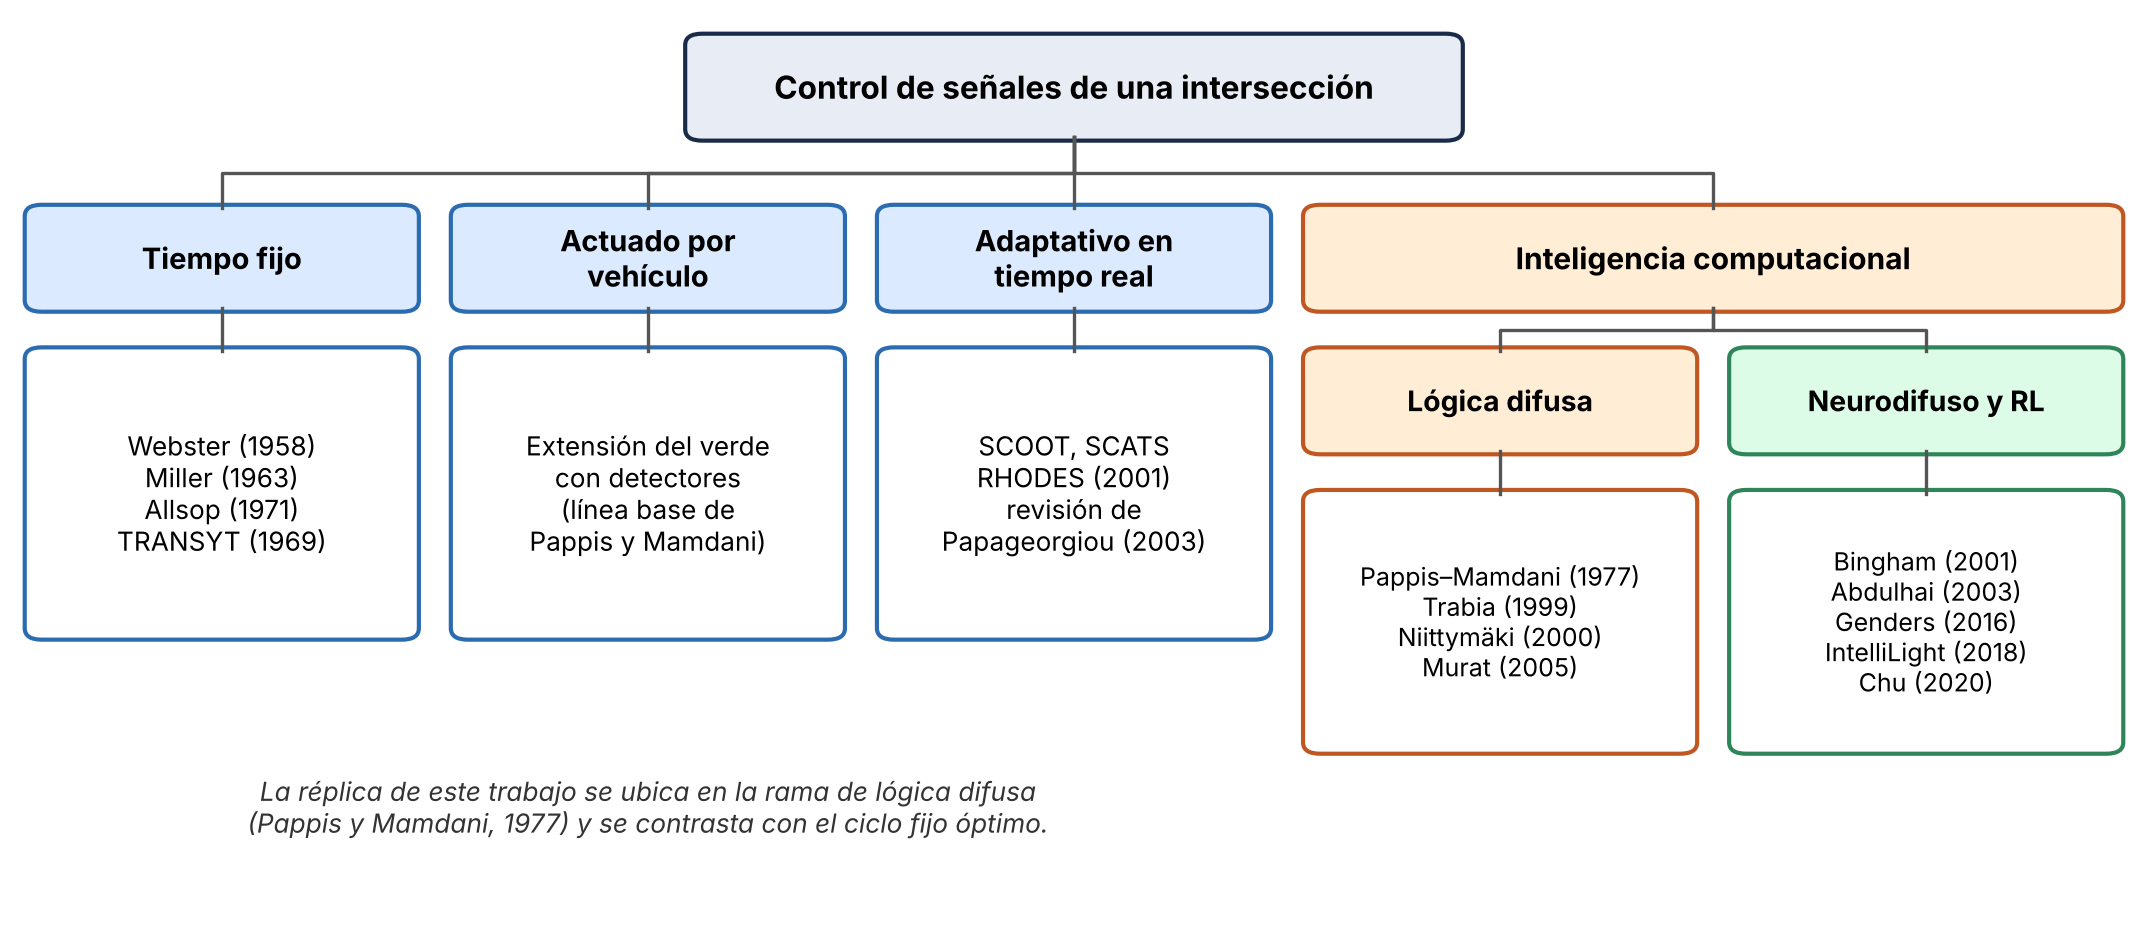
\includegraphics[width=\textwidth]{fig_taxonomia.png}
\caption{Taxonomía de los enfoques de control de una intersección aislada considerados en la revisión. La réplica se ubica en la rama de lógica difusa.}
\label{fig:taxonomia}
\end{figure*}

\begin{figure*}[!t]
\centering
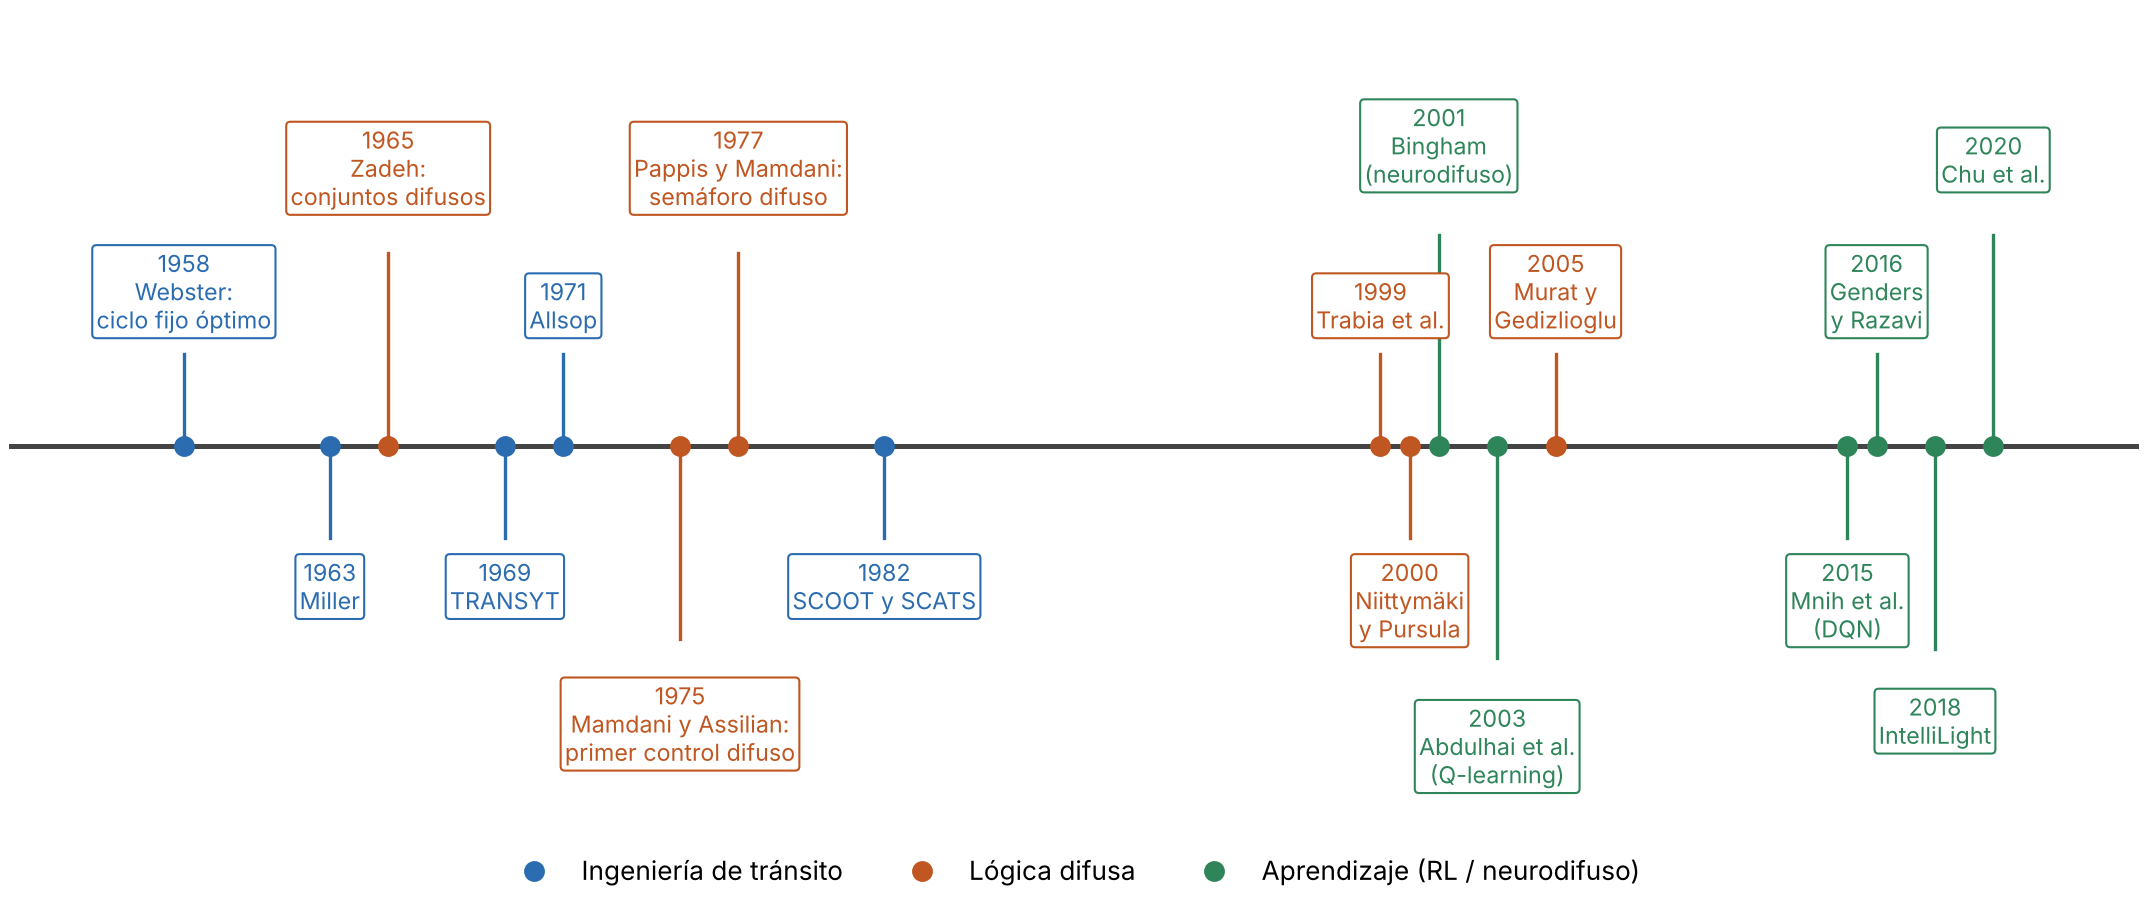
\includegraphics[width=\textwidth]{fig_timeline.png}
\caption{Línea de tiempo de las obras citadas: ingeniería de tránsito (azul), lógica difusa (naranja) y aprendizaje (verde).}
\label{fig:timeline}
\end{figure*}

\subsection{Control de una intersección aislada}
\label{sec:sota-aislada}

\subsubsection{Tiempo fijo}
El control de tiempo fijo repite un plan de ciclo y de verdes calculado a partir de los caudales medios. Webster \cite{Webster1958} dedujo el ciclo óptimo $C_0$ que minimiza el retardo,
\begin{equation}
C_0=\frac{1.5\,L+5}{1-Y},\qquad g_i=\frac{y_i}{Y}\,(C_0-L),
\label{eq:webster}
\end{equation}
donde $L$ es el tiempo perdido por ciclo, $y_i=q_i/s$ es la razón entre el caudal $q_i$ y el flujo de saturación $s$ de la fase $i$, $Y=\sum_i y_i$ y $g_i$ es el verde efectivo de la fase $i$. Origen: la expresión es la del artículo original (p.~709), tomada de Webster; el reparto $g_i$ y la cota $C>L/(1-Y)$ se deducen en el Sección~\ref{sec:formulas}, mientras que las constantes $1.5$ y $5$ son un ajuste empírico de Webster y no se deducen. Webster y Cobbe \cite{Webster1966} ampliaron el tratamiento de los semáforos, y Miller \cite{Miller1963} y Allsop \cite{Allsop1971} estudiaron los ajustes de ciclo fijo que minimizan el retardo en una intersección. TRANSYT \cite{Robertson1969} extiende la optimización de planes de tiempo fijo a una red. La limitación general, señalada por el propio Pappis y Mamdani, es que los retardos reales de un controlador de ciclo fijo exceden los óptimos cuando los caudales se apartan de aquellos para los que se calcularon los ajustes \cite{Pappis1977}.

\subsubsection{Control actuado por vehículo}
Un controlador actuado usa detectores para prolongar el verde mientras llegan vehículos, dentro de límites mínimo y máximo. Pappis y Mamdani lo toman como referencia: los retardos de su comparación final equivalen a los de un controlador actuado eficiente con ajustes óptimos \cite{Pappis1977}.

\subsubsection{Control adaptativo en tiempo real}
Los sistemas adaptativos optimizan en línea los parámetros de la señal con la información de detectores. SCOOT \cite{Hunt1982} y SCATS \cite{Lowrie1982} son los ejemplos más difundidos; RHODES \cite{Mirchandani2001} propone una arquitectura jerárquica que predice flujos de vehículos y pelotones y optimiza el control sobre un horizonte. Papageorgiou \emph{et al.} \cite{Papageorgiou2003} revisan las estrategias de control de tráfico urbano y de autopistas y las técnicas de guiado de rutas.

\begin{table}[!t]
\caption{Paradigmas de control de una intersección aislada}
\label{tab:paradigmas}
\centering
\footnotesize
\setlength{\tabcolsep}{3pt}
\begin{tabular}{@{}p{0.2\columnwidth}p{0.34\columnwidth}p{0.34\columnwidth}@{}}
\toprule
Paradigma & Información que usa & Limitación principal \\
\midrule
Tiempo fijo & Caudales medios, calculados fuera de línea & No responde a variaciones del tráfico \\
Actuado & Presencia de vehículos en detectores & Reglas fijas de extensión y límites \\
Adaptativo & Medidas en línea y predicción de flujo & Mayor infraestructura y modelo \\
Difuso & Variables lingüísticas (tiempo, arribos, cola) & Reglas obtenidas por prueba y error \\
Aprendizaje & Estado, acción y recompensa en simulación & Datos, cómputo y reproducibilidad \\
\bottomrule
\end{tabular}
\fuente{elaboración propia a partir de las obras citadas en las subsecciones del estado del arte: tiempo fijo \cite{Webster1958,Miller1963,Allsop1971,Robertson1969}, difuso \cite{Pappis1977} y aprendizaje \cite{Abdulhai2003,Genders2016}.}
\end{table}

\subsubsection{Medida de desempeño}
El retardo medio por vehículo es el criterio de desempeño de Pappis y Mamdani y de buena parte de la literatura posterior. Se define como el retardo total acumulado dividido por el número de vehículos,
\begin{equation}
d_m=\frac{D}{\sum_n q_n},
\label{eq:dm}
\end{equation}
con $q_n=1$ si llegó un vehículo en el $n$-ésimo segundo y $0$ en caso contrario \cite{Pappis1977}. Es la definición del artículo original (p.~708): el retardo total entre los vehículos llegados (Sección~\ref{sec:formulas}). La Tabla~\ref{tab:paradigmas} resume los paradigmas descritos.

\subsection{Lógica difusa y control lingüístico}
\label{sec:sota-difusa}

Zadeh \cite{Zadeh1965} introdujo los conjuntos difusos: a cada elemento $x$ de un universo se le asigna un grado de pertenencia $\mu_F(x)\in[0,1]$. Más tarde propuso un enfoque lingüístico para el análisis de sistemas complejos \cite{Zadeh1973} y el concepto de variable lingüística, cuyos valores son palabras como «pequeña» o «larga» \cite{Zadeh1975}. Esa base permitió expresar el conocimiento de un operador humano como reglas del tipo «si\,\dots\,entonces\,\dots».

Mamdani \cite{Mamdani1974} y Mamdani y Assilian \cite{MamdaniAssilian1975} aplicaron ese enfoque al control de una planta dinámica real, y Mamdani \cite{Mamdani1977} lo extendió al razonamiento aproximado mediante síntesis lingüística. En el esquema de Mamdani, el «y» de una regla se interpreta como mínimo y el «si no» entre reglas como máximo, de modo que el grado de la cláusula formada por $R$ reglas es
\begin{equation}
\mu_C(\mathbf{x},e)=\max_{r=1,\dots,R}\ \min\{\mu_{P_r}(\mathbf{x}),\ \mu_{E_r}(e)\},
\label{eq:mamdani}
\end{equation}
donde $\mu_{P_r}$ es la pertenencia del antecedente de la regla $r$ y $\mu_{E_r}$ la de su consecuente. Resulta de interpretar el «y» como mínimo y el «si no» como máximo, como hacen Pappis y Mamdani (p.~712); la deducción está en el Sección~\ref{sec:formulas}. Existen variantes posteriores: Takagi y Sugeno \cite{TakagiSugeno1985} usan consecuentes funcionales, y Jang \cite{Jang1993} integra un sistema de inferencia difusa en una red adaptativa cuyos parámetros se aprenden de datos. Lee \cite{Lee1990a,Lee1990b} ofrece una revisión de los componentes de un controlador difuso, entre ellos la fuzzificación, la base de reglas, el mecanismo de inferencia y los métodos de defuzzificación.

\subsection{Control difuso de semáforos}
\label{sec:sota-semaforos}

\subsubsection{El controlador de Pappis y Mamdani}
Pappis y Mamdani \cite{Pappis1977} estudian una intersección de dos calles unidireccionales (Fig.~\ref{fig:bloques}). Las llegadas se generan en cada segundo comparando un número pseudoaleatorio con la tasa media de arribo; el flujo de saturación es de 3600\,veh/h y el tiempo perdido, de 10\,s por ciclo. El modelo se valida con un controlador de ciclo fijo de ajustes óptimos, comparando el retardo simulado con la fórmula de Webster (Tabla~I del artículo original).

El retardo se contabiliza segundo a segundo. Sean $q_i\in\{0,1\}$ las llegadas, $Q_G$ los vehículos no despachados en el verde anterior y $Q_R$ la cola acumulada durante el rojo previo. La cola $n$ segundos después del inicio del rojo efectivo y el retardo acumulado durante el rojo ($R$ segundos) son
\begin{align}
Q_n &= Q_G+\sum_{i=1}^{n} q_i, \label{eq:colaR}\\
D_R &= \sum_{n=1}^{R}\Bigl(Q_G+\sum_{i=1}^{n} q_i\Bigr), \label{eq:retardoR}
\end{align}
y, durante el verde efectivo ($G$ segundos), los vehículos aún no despachados a flujo de saturación $s$ y el retardo que acumulan son
\begin{align}
S_n &= \Bigl[\,Q_R+\sum_{i=1}^{n} q_i-s\,n\Bigr]^{+}, \label{eq:colaG}\\
D_G &= \sum_{n=1}^{G} S_n, \qquad D=D_R+D_G, \label{eq:retardoG}
\end{align}
donde $[x]^{+}=\max\{x,0\}$. El retardo medio por vehículo se obtiene con \eqref{eq:dm}. Las ecuaciones \eqref{eq:colaR}--\eqref{eq:retardoG} son las del modelo del artículo original (p.~708); su deducción se da en el Sección~\ref{sec:formulas}.

\begin{figure*}[!t]
\centering
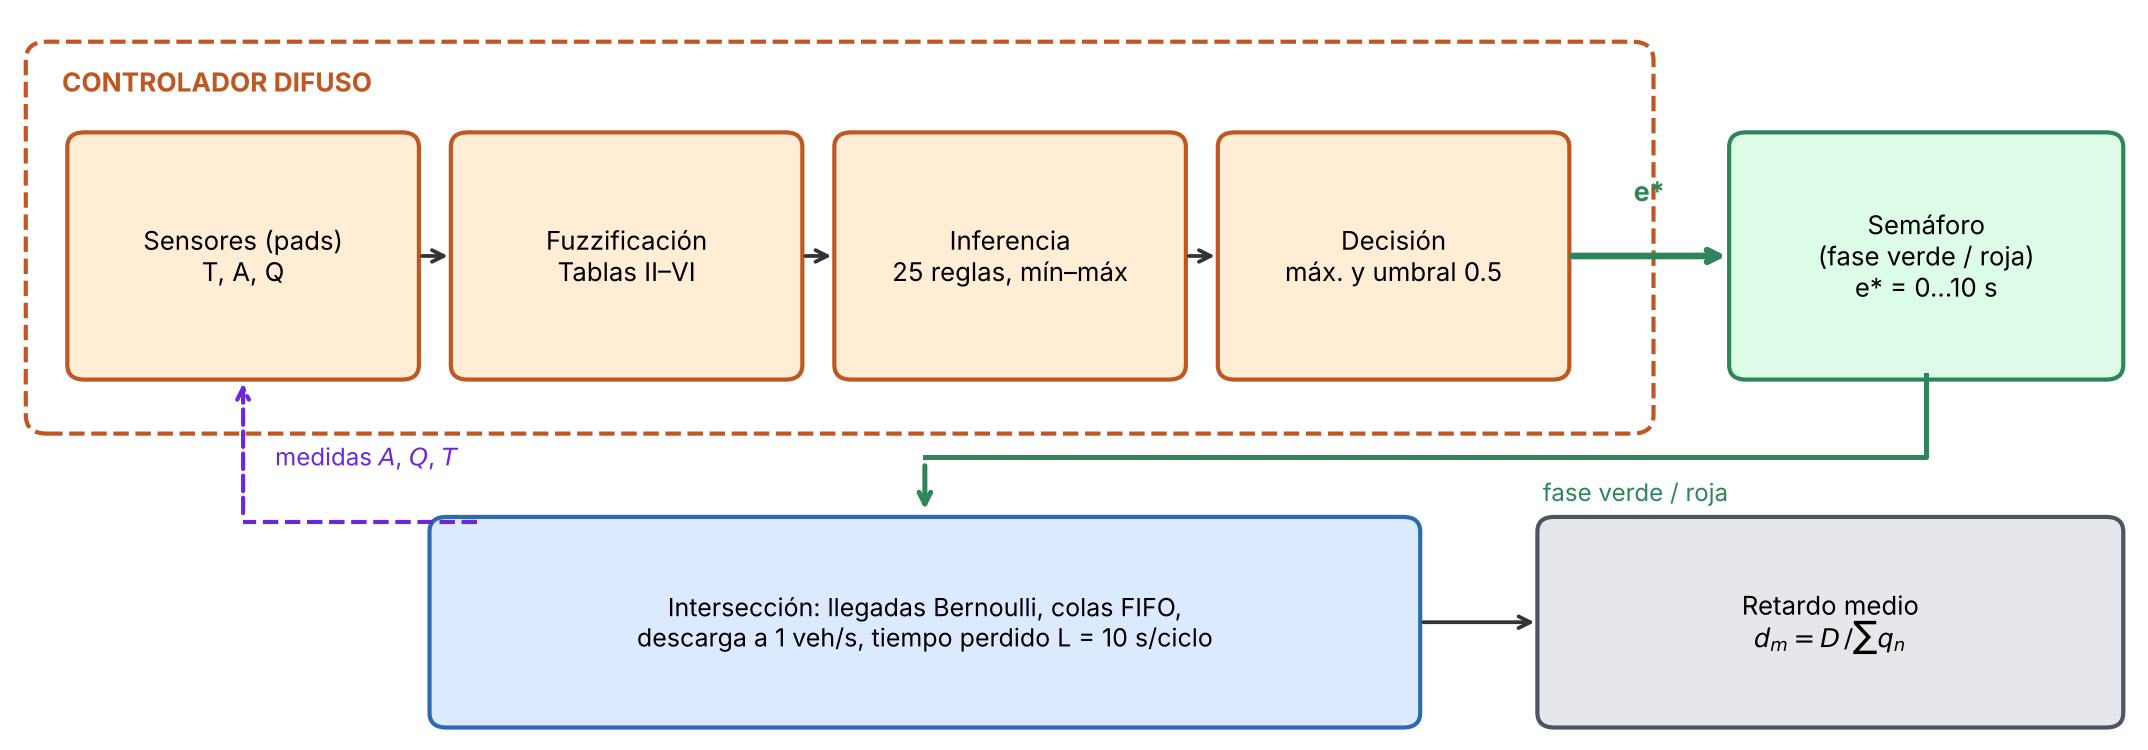
\includegraphics[width=\textwidth]{fig_bloques.png}
\caption{Diagrama de bloques del sistema de control de Pappis y Mamdani (elaboración propia a partir del artículo original).}
\label{fig:bloques}
\end{figure*}

El controlador interviene cada 10\,s durante el verde efectivo, la primera vez tras 7\,s, y decide la extensión $E$ del verde. Las entradas son el tiempo $T$ (la extensión candidata, de 1 a 10\,s), los arribos $A$ previstos en el brazo con derecho de paso y la cola $Q$ del brazo en rojo. Los valores lingüísticos se definen sobre universos discretos mediante tres tablas de conjuntos difusos, y dos operadores nuevos, «más que» (\emph{mt}) y «menos que» (\emph{lt}), generan versiones monótonas de esos conjuntos: dado el valor $x_0$ donde $\mu_A$ alcanza su máximo, $\mu_{lt(A)}(x)=1-\mu_A(x)$ si $x<x_0$ y $0$ en otro caso, y $\mu_{mt(A)}(x)=1-\mu_A(x)$ si $x>x_0$ y $0$ en otro caso \cite{Pappis1977}. La Fig.~\ref{fig:fuzzificacion} muestra los conjuntos reconstruidos para esta revisión.

\begin{figure*}[!t]
\centering
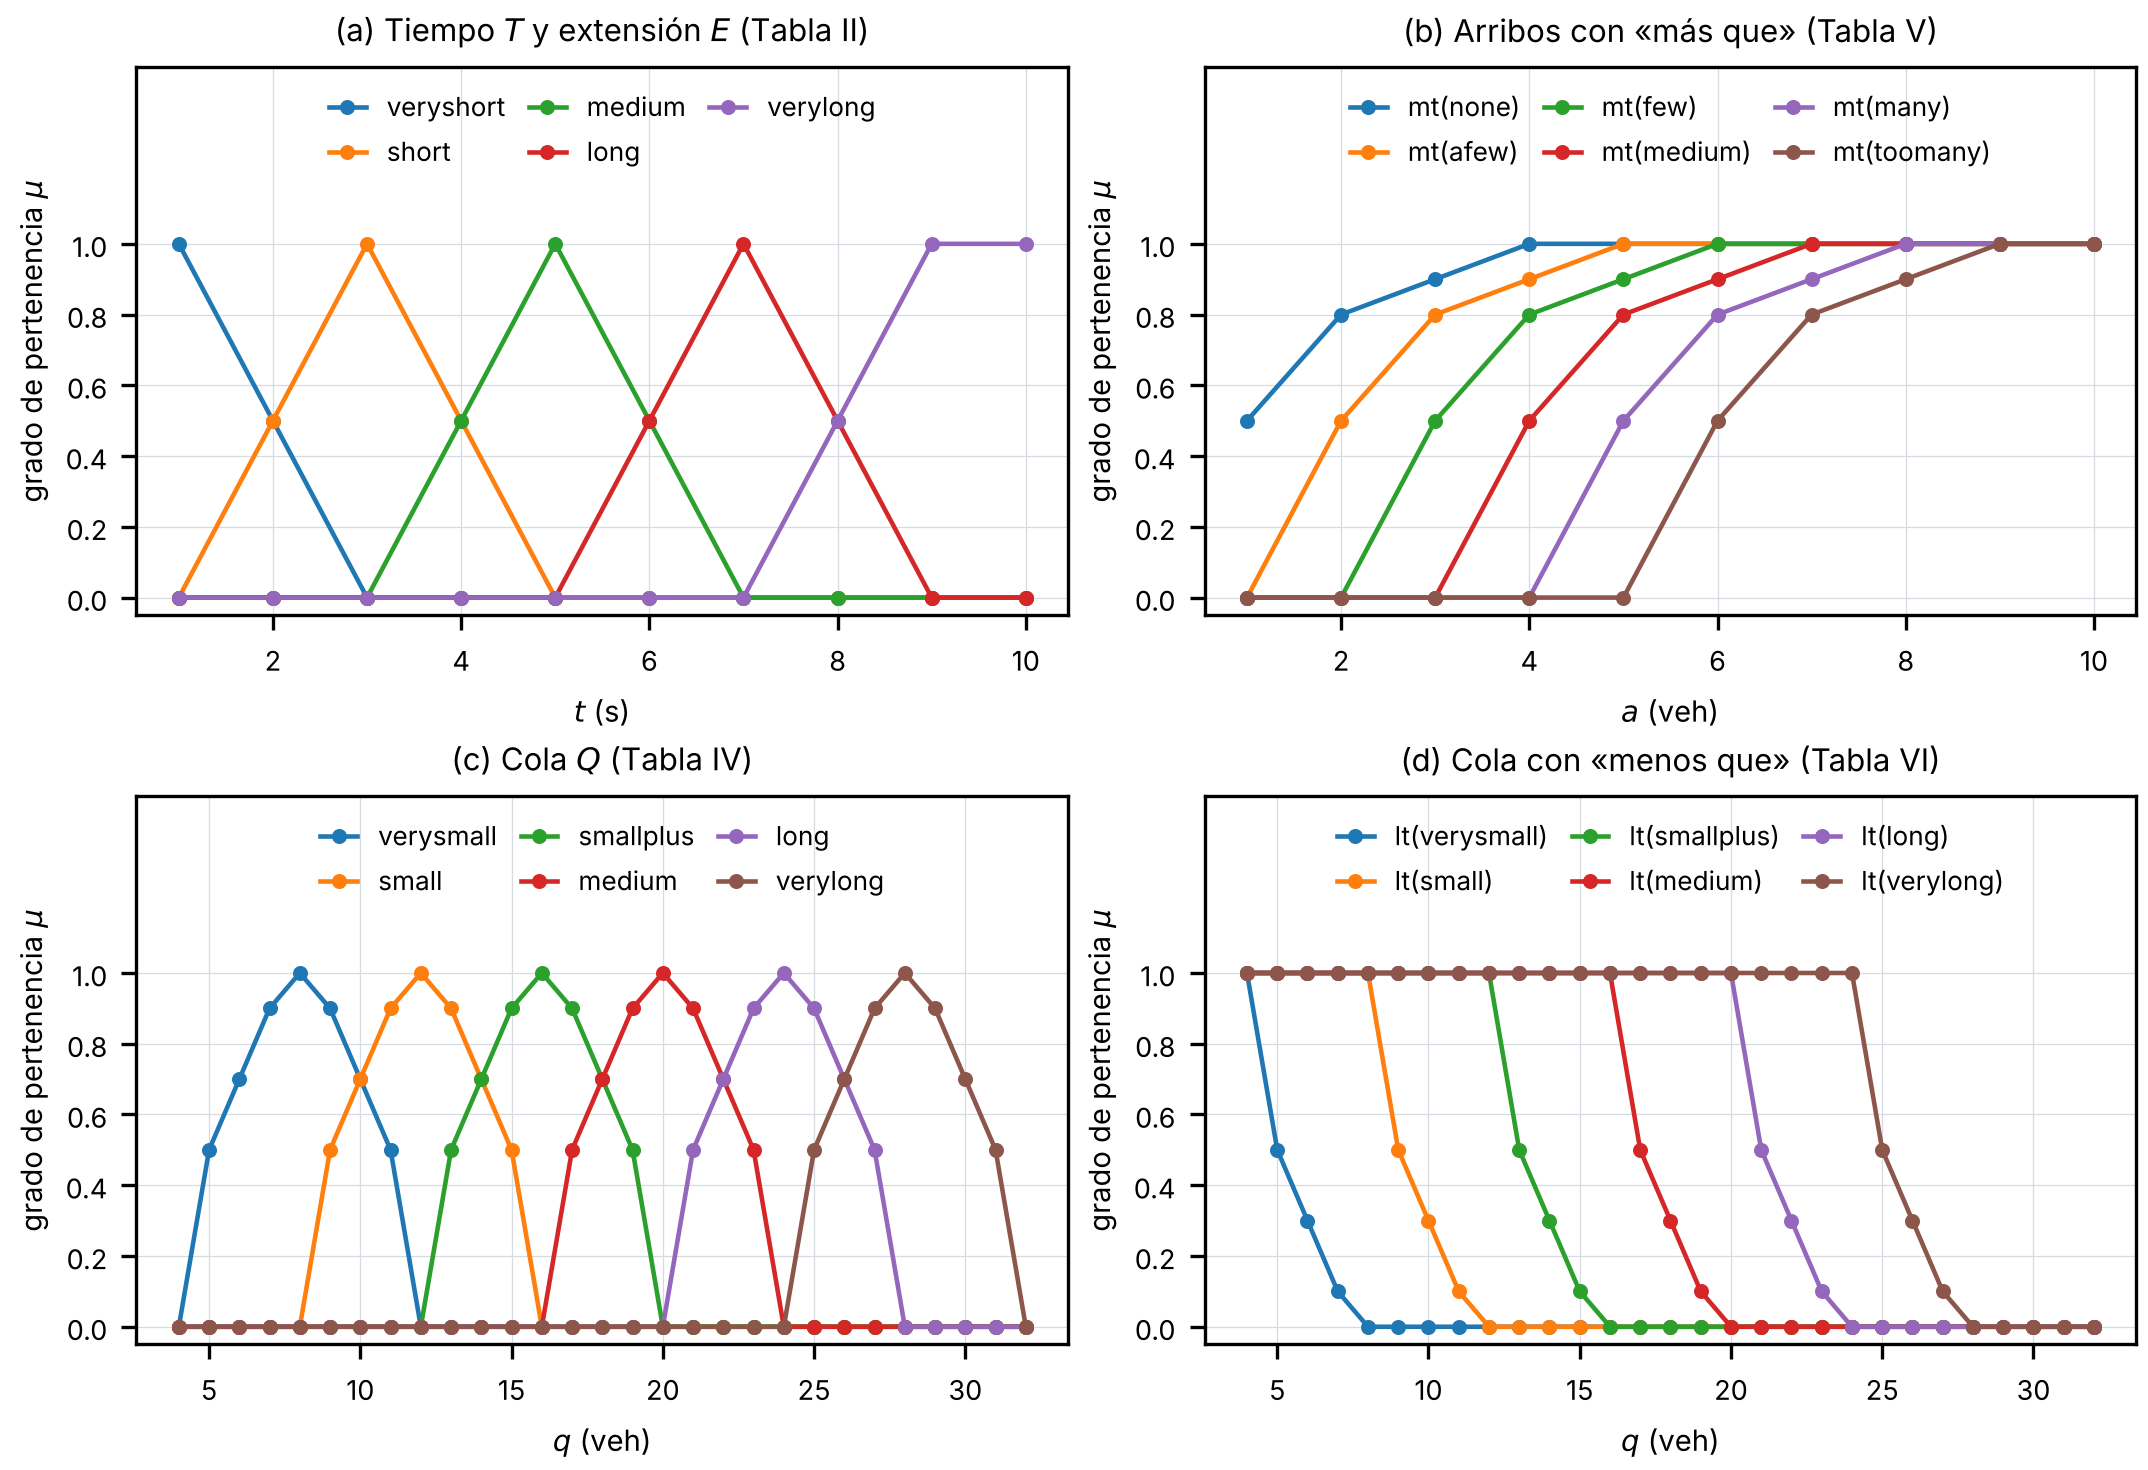
\includegraphics[width=\textwidth]{fig_fuzzificacion_ieee.png}
\caption{Curvas de fuzzificación del controlador de Pappis y Mamdani: (a) tiempo y extensión; (b) arribos con el operador «más que»; (c) colas; (d) colas con el operador «menos que». Trazadas con los valores impresos en el artículo original.}
\label{fig:fuzzificacion}
\end{figure*}

El conocimiento se expresa en 25 reglas, cinco por cada momento de intervención (7, 17, 27, 37 y 47\,s), con la forma
\begin{equation}
\text{si } T=t \text{ y } A=mt(a) \text{ y } Q=lt(q) \text{ entonces } E=e,
\end{equation}
donde en todas las reglas $T$ y $E$ comparten la misma etiqueta. Para cada $e=1,\dots,10$ se calcula el grado \eqref{eq:mamdani} con $\mu_{P_r}=\min\{\mu_T(e),\mu_{mt(A)}(a_e),\mu_{lt(Q)}(q_e)\}$, donde $a_e$ y $q_e$ son los arribos y la cola previstos para esa extensión. Se elige la extensión de mayor grado; si el máximo es menor que 0.5 no se extiende y se cambia de fase, y si el máximo no es único se toma la mayor extensión empatada. La defuzzificación es, por tanto, de tipo máximo con umbral, no un centroide. Con extensión de 10\,s se vuelve a intervenir al cabo de 10\,s, de modo que el verde efectivo no supera 57\,s.

Los resultados se resumen en una tabla que compara el retardo del controlador difuso con el del actuado eficaz para 16 combinaciones de caudal entre 360 y 2520\,veh/h; la mejora va de 10\,\% a 21\,\%. Los autores señalan que las reglas se afinaron por prueba y error y que fue el conjunto de reglas, y no los conjuntos difusos, lo que se modificó. Definen la estabilidad como la condición de no saturarse ante un amplio rango de caudales y observan que, una vez diseñado, el algoritmo actúa de forma determinista \cite{Pappis1977}.

\subsubsection{Trabajos posteriores}
La literatura posterior amplía el alcance del control difuso de semáforos. Trabia \emph{et al.} \cite{Trabia1999} proponen un controlador difuso de dos etapas que, con detectores de lazo, decide si extender o terminar la fase y lo comparan en simulación con un controlador actuado. Niittymäki y Pursula \cite{Niittymaki2000} desarrollan principios y algoritmos de control difuso de señales dentro de un proyecto de la Universidad Tecnológica de Helsinki. Murat y Gedizlioglu \cite{Murat2005} presentan FLMuSiC, un modelo con dos subsistemas difusos que fijan las duraciones de verde y la secuencia de fases a partir de los volúmenes de tráfico en una intersección aislada de cuatro accesos; en simulación mejora a un controlador actuado y al modelo aaSIDRA, sobre todo cuando los volúmenes varían más. Bingham \cite{Bingham2001} combina un controlador difuso con una red neuronal que ajusta las funciones de pertenencia mediante aprendizaje por refuerzo para reducir el retardo. La Tabla~\ref{tab:difusos} los resume.

\begin{table*}[!t]
\caption{Controladores difusos de semáforos considerados en la revisión}
\label{tab:difusos}
\centering
\footnotesize
\begin{tabular}{@{}p{0.10\textwidth}p{0.045\textwidth}p{0.40\textwidth}p{0.33\textwidth}@{}}
\toprule
Obra & Año & Idea principal & Evaluación reportada \\
\midrule
Pappis y Mamdani \cite{Pappis1977} & 1977 & Extensión del verde (1 a 10\,s) con 25 reglas lingüísticas sobre tiempo, arribos y cola & Simulación frente a actuado eficaz (equivalente a ciclo fijo óptimo): mejora de 10\,\% a 21\,\% \\
Trabia \emph{et al.} \cite{Trabia1999} & 1999 & Controlador difuso de dos etapas con detectores de lazo que decide extender o terminar la fase & Simulación de una intersección de cuatro accesos frente a un controlador actuado \\
Niittymäki y Pursula \cite{Niittymaki2000} & 2000 & Principios y algoritmos de control difuso de señales (proyecto FUSICO, Helsinki) & Ver la referencia \\
Bingham \cite{Bingham2001} & 2001 & Controlador neurodifuso: una red ajusta las funciones de pertenencia por aprendizaje por refuerzo & Simulación con volúmenes constantes: menor retardo que las funciones iniciales \\
Murat y Gedizlioglu \cite{Murat2005} & 2005 & FLMuSiC: dos subsistemas difusos fijan duraciones de verde y secuencia de fases según volúmenes & Intersección de cuatro accesos frente a actuado simulado y aaSIDRA: menor retardo, sobre todo con volúmenes variables \\
\bottomrule
\end{tabular}
\fuente{obras citadas en la columna «Obra»; cada fila resume la referencia correspondiente. La mejora de Pappis y Mamdani es la columna «Improvement» impresa en su Tabla~VIII (p.~715), de +10\,\% a +21\,\%.}
\end{table*}

En conjunto, las obras revisadas conservan la estructura lingüística de Pappis y Mamdani (variables de tráfico, reglas «si–entonces», inferencia mínimo–máximo), pero aumentan el número de fases controladas, incorporan la decisión de secuencia de fases y, en el caso neurodifuso, sustituyen el ajuste manual de las funciones de pertenencia por un ajuste aprendido \cite{Murat2005,Bingham2001}.

\subsection{Aprendizaje por refuerzo y aprendizaje profundo}
\label{sec:sota-rl}

Una línea paralela formula el control de semáforos como un problema de decisión secuencial. Wiering \cite{Wiering2000} propone aprendizaje por refuerzo multiagente para el control de semáforos, y Abdulhai \emph{et al.} \cite{Abdulhai2003} aplican \emph{Q-learning} a una intersección aislada con tráfico variable. El aprendizaje profundo por refuerzo \cite{Mnih2015} se traslada después a este dominio: Genders y Razavi \cite{Genders2016} entrenan una red convolucional con \emph{Q-learning} y repetición de experiencia en el simulador SUMO con una codificación discreta del estado, IntelliLight \cite{Wei2018} se evalúa con datos reales obtenidos de cámaras de vigilancia, y Chu \emph{et al.} \cite{Chu2020} proponen una variante descentralizada y multiagente de \emph{advantage actor-critic} evaluada en una malla sintética y en una red real de Mónaco. Yau \emph{et al.} \cite{Yau2017} revisan estos modelos según la representación del estado, la acción y la recompensa, y las medidas de desempeño; Wei \emph{et al.} \cite{Wei2019} revisan los métodos de control de semáforos, incluidos los basados en aprendizaje.

\begin{table}[!t]
\caption{Trabajos de aprendizaje por refuerzo considerados en la revisión}
\label{tab:rl}
\centering
\footnotesize
\setlength{\tabcolsep}{3pt}
\begin{tabular}{@{}p{0.27\columnwidth}p{0.08\columnwidth}p{0.55\columnwidth}@{}}
\toprule
Obra & Año & Método y evaluación \\
\midrule
Wiering \cite{Wiering2000} & 2000 & Aprendizaje por refuerzo multiagente para semáforos \\
Abdulhai \emph{et al.} \cite{Abdulhai2003} & 2003 & \emph{Q-learning}; intersección aislada con tráfico variable \\
Genders y Razavi \cite{Genders2016} & 2016 & Red convolucional con \emph{Q-learning} y repetición de experiencia; simulador SUMO \\
Wei \emph{et al.} \cite{Wei2018} & 2018 & IntelliLight; datos reales de cámaras de vigilancia \\
Chu \emph{et al.} \cite{Chu2020} & 2020 & \emph{Advantage actor-critic} multiagente descentralizado; malla sintética y red de Mónaco \\
\bottomrule
\end{tabular}
\fuente{obras citadas en la columna «Obra»; cada fila resume la referencia correspondiente.}
\end{table}

Frente a las reglas escritas por una persona, estos métodos aprenden la política de datos y simulaciones, pero dependen de la definición de estado y recompensa, del simulador y de hiperparámetros, aspectos cuya documentación incompleta dificulta la comparación entre estudios \cite{Henderson2018}.

\subsection{Reproducibilidad y réplica}
\label{sec:sota-repro}

La reproducibilidad computacional es una preocupación creciente. Peng \cite{Peng2011} la plantea como un espectro que va de la mera publicación del artículo a la réplica completa, pasando por la liberación del código y de los datos, y Sandve \emph{et al.} \cite{Sandve2013} proponen diez reglas simples para investigación computacional reproducible. En inteligencia artificial, Gundersen y Kjensmo \cite{Gundersen2018} revisan 400 artículos de IJCAI y AAAI y encuentran que entre 20\,\% y 30\,\% de las variables de cada factor están documentadas; Henderson \emph{et al.} \cite{Henderson2018} muestran que la no determinación de los entornos y la varianza de los métodos pueden alterar la interpretación de los resultados; Pineau \emph{et al.} \cite{Pineau2021} describen un programa de reproducibilidad con política de código, desafío comunitario y lista de verificación.

Un trabajo de 1977 enfrenta una dificultad extrema: no hay código, el generador aleatorio es distinto y los parámetros de la simulación no se publicaron. La réplica solo puede ser estadística y debe separar con claridad lo que el artículo \emph{especifica} de lo que el replicador \emph{infiere}.

\subsection{Síntesis y brecha}
\label{sec:sota-brecha}

La revisión muestra que el controlador de Pappis y Mamdani es un antecedente de las líneas difusa, neurodifusa y de aprendizaje, pero no se encontró una validación pública de su implementación. En las fuentes consultadas para esta revisión no se encontró una réplica documentada del controlador original, ni una auditoría de qué partes de su descripción bastan para reproducir sus resultados. Este trabajo cubre esa brecha: implementa el controlador desde la publicación original, valida cada elemento impreso, identifica qué datos faltan y declara como inferencia la única lectura de las entradas compatible con los resultados.

% =============================================================================
\section{Fundamentos del controlador}
\label{sec:fundamentos}

Esta sección describe el controlador tal como lo define el artículo original \cite{Pappis1977}. Todos los valores numéricos se transcribieron de las imágenes de sus tablas.

\subsection{Variables y universos}
El controlador usa tres variables de entrada y una de salida, todas definidas sobre universos discretos (Tabla~\ref{tab:variables}). El tiempo $T$ es la extensión candidata del verde en segundos y la extensión $E$ toma los mismos valores lingüísticos que $T$. Los arribos $A$ son los vehículos que cruzarán el punto crítico en los $t$ segundos siguientes, y la cola $Q$ es el número de vehículos esperando en el brazo en rojo.

\begin{table}[!t]
\caption{Variables difusas del controlador}
\label{tab:variables}
\centering
\footnotesize
\setlength{\tabcolsep}{3pt}
\begin{tabular}{@{}p{0.2\columnwidth}p{0.22\columnwidth}p{0.46\columnwidth}@{}}
\toprule
Variable & Universo & Valores lingüísticos \\
\midrule
$T$ y $E$ & $t=1,\dots,10$\,s & very short, short, medium, long, very long \\
$A$ & $a=1,\dots,10$\,veh & none, a few, few, medium, many, too many \\
$Q$ & $q=4,\dots,32$\,veh & very small, small, small plus, medium, long, very long \\
\bottomrule
\end{tabular}
\fuente{Tablas~II a~IV del artículo original (p.~711): universos y etiquetas lingüísticas de $T$, $E$, $A$ y $Q$.}
\end{table}

\subsection{Conjuntos y operadores «más que» y «menos que»}
Los valores lingüísticos se definen mediante las Tablas~II a~IV del artículo original; sus curvas se muestran en la Fig.~\ref{fig:fuzzificacion}. Las reglas no usan esos conjuntos directamente, sino versiones monótonas obtenidas con dos operadores. Sea $x_0$ el elemento del universo donde $\mu_A$ alcanza su máximo. Las definiciones son las del artículo original (p.~710) y sus propiedades se demuestran en el Sección~\ref{sec:formulas}:
\begin{align}
\mu_{lt(A)}(x)&=\begin{cases}1-\mu_A(x), & x<x_0\\ 0, & x\ge x_0\end{cases} \label{eq:lt}\\
\mu_{mt(A)}(x)&=\begin{cases}0, & x\le x_0\\ 1-\mu_A(x), & x>x_0\end{cases} \label{eq:mt}
\end{align}
La Tabla~V del artículo imprime $\mu_{mt(\text{none})}(1)=0.5$, es decir, $1-\mu_A(x_0)$ cuando el máximo es menor que 1; el código sigue los valores impresos. Fuera de los universos se adoptaron dos supuestos, declarados también en la Sección~\ref{sec:discusion}: $\mu_{lt(\cdot)}(q)=1$ para $q<4$ y $\mu_{mt(\cdot)}(0)=0$. El conjunto «any» vale 1 en todo su universo.

\subsection{Base de reglas}
El conocimiento del controlador son 25 reglas «si $T=t$ y $A=mt(a)$ y $Q=lt(q)$ entonces $E=e$», cinco por cada momento de intervención (7, 17, 27, 37 y 47\,s). La Tabla~\ref{tab:reglas} las resume. Dentro de cada intervención hay una regla por etiqueta de salida; a mayor extensión, la regla exige más arribos y admite menos cola en el brazo en rojo. Al aumentar el tiempo de verde, los umbrales de cola se vuelven más permisivos (de \emph{very small} a \emph{very long}), pues la cola del brazo en rojo crece de forma natural con el tiempo. El Apéndice~\ref{app:180} escribe, una por una, las 180 reglas posibles de $T$, $A$ y $Q$ y resalta en verde las que usa el autor: las 25 reglas ocupan solo 19 de las 180, porque varias se repiten en distintas intervenciones y la regla R1 no condiciona la cola (usa \emph{any}, y cubre las seis colas de su fila).

\begin{table*}[!t]
\caption{Desglose de las 25 reglas del Apéndice del artículo original: cada columna es una intervención y cada caja una regla, con sus condiciones sobre $T$, $A$ y $Q$ y su conclusión $E=T$. R5 es la que más extiende el verde.}
\label{tab:reglas}
\centering
\scriptsize
\setlength{\tabcolsep}{7pt}
\renewcommand{\arraystretch}{1.05}
\begin{tabular}{@{}ccccc@{}}
\toprule
7\,s & 17\,s & 27\,s & 37\,s & 47\,s \\
\midrule
\begin{tabular}[t]{@{}l@{}}\textbf{R1} \\ \textbf{SI} $T$ = very short \\ \textbf{Y} $A$ = mt(none) \\ \textbf{Y} $Q$ = any \\ \textbf{ENTONCES} $E$ = very short\end{tabular} & \begin{tabular}[t]{@{}l@{}}\textbf{R1} \\ \textbf{SI} $T$ = very short \\ \textbf{Y} $A$ = mt(none) \\ \textbf{Y} $Q$ = any \\ \textbf{ENTONCES} $E$ = very short\end{tabular} & \begin{tabular}[t]{@{}l@{}}\textbf{R1} \\ \textbf{SI} $T$ = very short \\ \textbf{Y} $A$ = mt(none) \\ \textbf{Y} $Q$ = any \\ \textbf{ENTONCES} $E$ = very short\end{tabular} & \begin{tabular}[t]{@{}l@{}}\textbf{R1} \\ \textbf{SI} $T$ = very short \\ \textbf{Y} $A$ = mt(none) \\ \textbf{Y} $Q$ = any \\ \textbf{ENTONCES} $E$ = very short\end{tabular} & \begin{tabular}[t]{@{}l@{}}\textbf{R1} \\ \textbf{SI} $T$ = very short \\ \textbf{Y} $A$ = mt(none) \\ \textbf{Y} $Q$ = any \\ \textbf{ENTONCES} $E$ = very short\end{tabular} \\
\midrule
\begin{tabular}[t]{@{}l@{}}\textbf{R2} \\ \textbf{SI} $T$ = short \\ \textbf{Y} $A$ = mt(a few) \\ \textbf{Y} $Q$ = lt(very small) \\ \textbf{ENTONCES} $E$ = short\end{tabular} & \begin{tabular}[t]{@{}l@{}}\textbf{R2} \\ \textbf{SI} $T$ = short \\ \textbf{Y} $A$ = mt(a few) \\ \textbf{Y} $Q$ = lt(very small) \\ \textbf{ENTONCES} $E$ = short\end{tabular} & \begin{tabular}[t]{@{}l@{}}\textbf{R2} \\ \textbf{SI} $T$ = short \\ \textbf{Y} $A$ = mt(a few) \\ \textbf{Y} $Q$ = lt(very small) \\ \textbf{ENTONCES} $E$ = short\end{tabular} & \begin{tabular}[t]{@{}l@{}}\textbf{R2} \\ \textbf{SI} $T$ = short \\ \textbf{Y} $A$ = mt(a few) \\ \textbf{Y} $Q$ = lt(small plus) \\ \textbf{ENTONCES} $E$ = short\end{tabular} & \begin{tabular}[t]{@{}l@{}}\textbf{R2} \\ \textbf{SI} $T$ = short \\ \textbf{Y} $A$ = mt(a few) \\ \textbf{Y} $Q$ = lt(long) \\ \textbf{ENTONCES} $E$ = short\end{tabular} \\
\midrule
\begin{tabular}[t]{@{}l@{}}\textbf{R3} \\ \textbf{SI} $T$ = medium \\ \textbf{Y} $A$ = mt(few) \\ \textbf{Y} $Q$ = lt(very small) \\ \textbf{ENTONCES} $E$ = medium\end{tabular} & \begin{tabular}[t]{@{}l@{}}\textbf{R3} \\ \textbf{SI} $T$ = medium \\ \textbf{Y} $A$ = mt(few) \\ \textbf{Y} $Q$ = lt(very small) \\ \textbf{ENTONCES} $E$ = medium\end{tabular} & \begin{tabular}[t]{@{}l@{}}\textbf{R3} \\ \textbf{SI} $T$ = medium \\ \textbf{Y} $A$ = mt(few) \\ \textbf{Y} $Q$ = lt(very small) \\ \textbf{ENTONCES} $E$ = medium\end{tabular} & \begin{tabular}[t]{@{}l@{}}\textbf{R3} \\ \textbf{SI} $T$ = medium \\ \textbf{Y} $A$ = mt(medium) \\ \textbf{Y} $Q$ = lt(small plus) \\ \textbf{ENTONCES} $E$ = medium\end{tabular} & \begin{tabular}[t]{@{}l@{}}\textbf{R3} \\ \textbf{SI} $T$ = medium \\ \textbf{Y} $A$ = mt(medium) \\ \textbf{Y} $Q$ = lt(long) \\ \textbf{ENTONCES} $E$ = medium\end{tabular} \\
\midrule
\begin{tabular}[t]{@{}l@{}}\textbf{R4} \\ \textbf{SI} $T$ = long \\ \textbf{Y} $A$ = mt(medium) \\ \textbf{Y} $Q$ = lt(very small) \\ \textbf{ENTONCES} $E$ = long\end{tabular} & \begin{tabular}[t]{@{}l@{}}\textbf{R4} \\ \textbf{SI} $T$ = long \\ \textbf{Y} $A$ = mt(medium) \\ \textbf{Y} $Q$ = lt(very small) \\ \textbf{ENTONCES} $E$ = long\end{tabular} & \begin{tabular}[t]{@{}l@{}}\textbf{R4} \\ \textbf{SI} $T$ = long \\ \textbf{Y} $A$ = mt(medium) \\ \textbf{Y} $Q$ = lt(very small) \\ \textbf{ENTONCES} $E$ = long\end{tabular} & \begin{tabular}[t]{@{}l@{}}\textbf{R4} \\ \textbf{SI} $T$ = long \\ \textbf{Y} $A$ = mt(many) \\ \textbf{Y} $Q$ = lt(medium) \\ \textbf{ENTONCES} $E$ = long\end{tabular} & \begin{tabular}[t]{@{}l@{}}\textbf{R4} \\ \textbf{SI} $T$ = long \\ \textbf{Y} $A$ = mt(too many) \\ \textbf{Y} $Q$ = lt(very long) \\ \textbf{ENTONCES} $E$ = long\end{tabular} \\
\midrule
\begin{tabular}[t]{@{}l@{}}\textbf{R5} \\ \textbf{SI} $T$ = very long \\ \textbf{Y} $A$ = mt(many) \\ \textbf{Y} $Q$ = lt(very small) \\ \textbf{ENTONCES} $E$ = very long\end{tabular} & \begin{tabular}[t]{@{}l@{}}\textbf{R5} \\ \textbf{SI} $T$ = very long \\ \textbf{Y} $A$ = mt(many) \\ \textbf{Y} $Q$ = lt(small) \\ \textbf{ENTONCES} $E$ = very long\end{tabular} & \begin{tabular}[t]{@{}l@{}}\textbf{R5} \\ \textbf{SI} $T$ = very long \\ \textbf{Y} $A$ = mt(many) \\ \textbf{Y} $Q$ = lt(small) \\ \textbf{ENTONCES} $E$ = very long\end{tabular} & \begin{tabular}[t]{@{}l@{}}\textbf{R5} \\ \textbf{SI} $T$ = very long \\ \textbf{Y} $A$ = mt(too many) \\ \textbf{Y} $Q$ = lt(long) \\ \textbf{ENTONCES} $E$ = very long\end{tabular} & \begin{tabular}[t]{@{}l@{}}\textbf{R5} \\ \textbf{SI} $T$ = very long \\ \textbf{Y} $A$ = mt(too many) \\ \textbf{Y} $Q$ = lt(very long) \\ \textbf{ENTONCES} $E$ = very long\end{tabular} \\
\bottomrule
\end{tabular}
\end{table*}



\subsection{Inferencia y decisión}
Para cada extensión candidata $e=1,\dots,10$\,s, la regla $r$ aporta el grado
\begin{equation}
\mu_{P_r}(e)=\min\{\mu_{T_r}(e),\ \mu_{mt(A_r)}(a_e),\ \mu_{lt(Q_r)}(q_e),\ \mu_{E_r}(e)\},
\label{eq:premisa}
\end{equation}
donde $a_e$ y $q_e$ son los arribos y la cola evaluados para esa extensión (Sección~\ref{sec:lecturas}). El grado del algoritmo es $g(e)=\max_r\mu_{P_r}(e)$, la unión de las reglas con el operador máximo (ecuación~\eqref{eq:mamdani}); sea $g_{\max}=\max_k g(k)$. La decisión no usa centroide:
\begin{equation}
e^*=\begin{cases}\max\{e:\ g(e)=g_{\max}\}, & g_{\max}\ge 0.5\\ 0, & g_{\max}<0.5\end{cases}
\label{eq:decision}
\end{equation}
Con $e^*=0$ se cambia de fase de inmediato. El desempate toma la mayor extensión, como indica el artículo original. Si $e^*=10$ se vuelve a intervenir 10\,s después; si $0<e^*<10$ el verde termina tras $e^*$ segundos. Se llama \emph{activación} de una regla al máximo de $\mu_{P_r}(e)$ sobre $e$, y \emph{disparo} a que la regla cuya contribución en $e^*$ iguala el grado máximo; un corte del verde no tiene regla que dispare. Las ecuaciones \eqref{eq:premisa} y \eqref{eq:decision} formalizan lo descrito en las pp.~712 a~714 del artículo original; su deducción se da en el Sección~\ref{sec:formulas}.

\subsection{Ejemplo trabajado del artículo original}
\label{sec:ejemplo}
El artículo ilustra la decisión con la segunda intervención (17\,s). Los arribos del brazo con paso son $\mathbf{x}=(0\,1\,0\,1\,1\,1\,1\,0\,0\,1)$, con acumulados $\beta=(0\,1\,1\,2\,3\,4\,5\,5\,5\,6)$; los del brazo en rojo, $\mathbf{x}'=(0\,1\,0\,0\,1\,0\,0\,1\,0\,0)$, con cola inicial $Q=5$ y cola prevista $\beta'=(5\,6\,6\,6\,7\,7\,7\,8\,8\,8)$. Con esos vectores, el grado del algoritmo es $(0,\,0.5,\,0,\,0.3,\,0.1,\,0.1,\,0.1,\,0.5,\,0.5,\,0.8)$ y la extensión elegida es $e^*=10$\,s. La Tabla~\ref{tab:tabla7} y la Fig.~\ref{fig:tabla7} muestran la contribución de cada regla.

\begin{table}[!t]
\caption{Ejemplo del artículo original (17\,s): aporte de cada regla para cada extensión $e$ (s). Coincide con la Tabla~VII del artículo.}
\label{tab:tabla7}
\centering
\scriptsize
\setlength{\tabcolsep}{2.2pt}
\begin{tabular}{@{}l*{10}{c}@{}}
\toprule
 & 1 & 2 & 3 & 4 & 5 & 6 & 7 & 8 & 9 & 10 \\
\midrule
R1 very short & 0 & 0.5 & 0 & 0 & 0 & 0 & 0 & 0 & 0 & 0 \\
R2 short & 0 & 0 & 0 & 0.3 & 0 & 0 & 0 & 0 & 0 & 0 \\
R3 medium & 0 & 0 & 0 & 0 & 0.1 & 0.1 & 0 & 0 & 0 & 0 \\
R4 long & 0 & 0 & 0 & 0 & 0 & 0.1 & 0.1 & 0 & 0 & 0 \\
R5 very long & 0 & 0 & 0 & 0 & 0 & 0 & 0 & 0.5 & 0.5 & 0.8 \\
\midrule
Algoritmo & \textbf{0} & \textbf{0.5} & \textbf{0} & \textbf{0.3} & \textbf{0.1} & \textbf{0.1} & \textbf{0.1} & \textbf{0.5} & \textbf{0.5} & \textbf{0.8} \\
\bottomrule
\end{tabular}
\end{table}


\begin{figure}[!t]
\centering
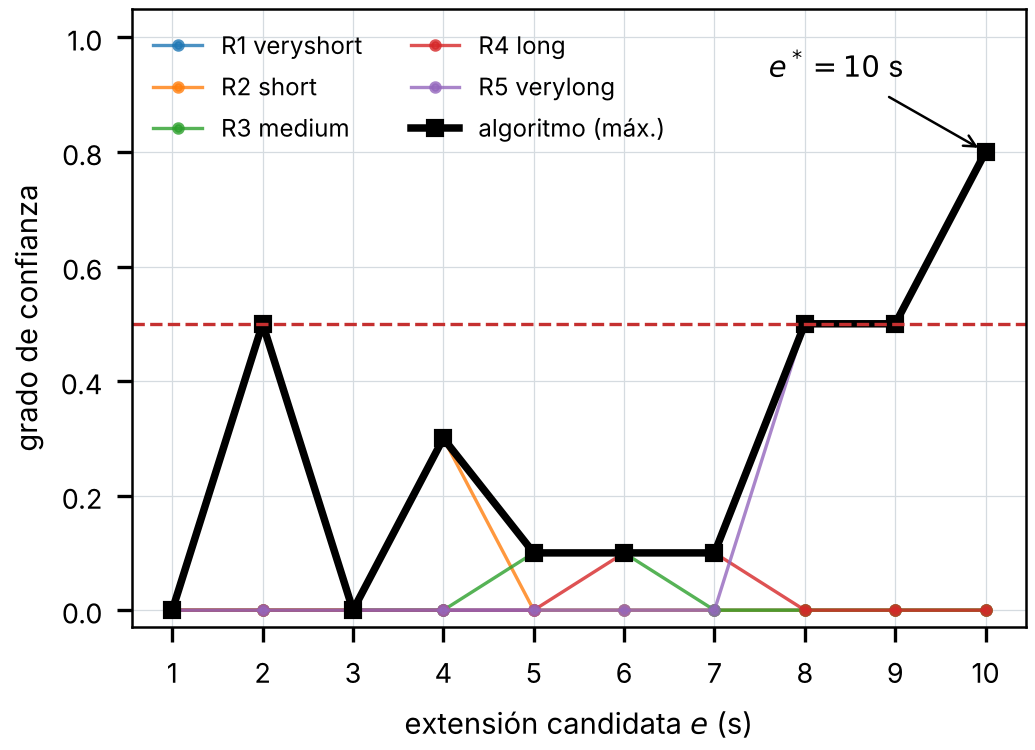
\includegraphics[width=\columnwidth]{fig_tabla7.png}
\caption{Ejemplo de las págs. 7--8 del artículo original (intervención de 17\,s): contribución de cada regla y grado agregado. El máximo (0.8 en $e=10$\,s) supera el umbral 0.5.}
\label{fig:tabla7}
\end{figure}

% =============================================================================
\section{Desarrollo matemático de las fórmulas}
\label{sec:formulas}
Esta sección muestra de dónde nace cada fórmula del artículo. Cada una es de una de tres clases: (i) \emph{del artículo original}, con la página en que aparece; (ii) \emph{deducida} aquí a partir de definiciones o de las hipótesis del modelo, con el desarrollo paso a paso; o (iii) \emph{empírica o inferida}, lo que se declara. La Tabla~\ref{tab:origen-formulas} resume el origen de cada fórmula; los apartados siguientes dan los desarrollos y la Sección~\ref{sec:verif-formulas} los comprueba con cálculos numéricos independientes. Las páginas se refieren al artículo de Pappis y Mamdani \cite{Pappis1977}.

\begin{table*}[!t]
\caption{Origen de cada fórmula del artículo}
\label{tab:origen-formulas}
\centering
\footnotesize
\setlength{\tabcolsep}{3pt}
\begin{tabular}{@{}p{0.2\textwidth}p{0.22\textwidth}p{0.5\textwidth}@{}}
\toprule
Fórmula & Procedencia & Qué se deduce y qué no \\
\midrule
\eqref{eq:colaR}, \eqref{eq:retardoR} (cola y retardo en el rojo) & Artículo original, p.~708 & Deducidas por acumulación de llegadas e intercambio de sumas (Sección~\ref{ap:colas}) \\
\eqref{eq:colaG}, \eqref{eq:retardoG} (cola y retardo en el verde) & Artículo original, p.~708 & Deducidas por inducción, con descarga a flujo de saturación (Sección~\ref{ap:colas}) \\
\eqref{eq:dm} (retardo medio) & Artículo original, p.~708 & Definición de media: retardo total entre vehículos llegados \\
\eqref{eq:retardo-webster} (retardo de Webster) & Artículo original, p.~709, de Webster \cite{Webster1958} & Primer término (cola uniforme) y segundo término (cola M/D/1) deducidos (Sección~\ref{ap:webster}); el tercero es una corrección empírica de Webster, no deducida \\
\eqref{eq:webster} (ciclo y verdes óptimos) & Artículo original, p.~709, de Webster \cite{Webster1958} & Reparto $g_i$ y cota $C>L/(1-Y)$ deducidos (Sección~\ref{ap:ciclo}); constantes $1.5$ y $5$ empíricas \\
\eqref{eq:lt}, \eqref{eq:mt} (operadores) & Artículo original, p.~710 & Definiciones; sus dos propiedades se demuestran (Sección~\ref{ap:mtlt}) \\
\eqref{eq:mamdani}, \eqref{eq:premisa} (inferencia) & Artículo original, pp.~710 a~713 & Deducidas de «y»$=$mínimo, «si no»$=$máximo y de la regla composicional con entradas exactas (Sección~\ref{ap:inferencia}) \\
\eqref{eq:decision} (decisión) & Artículo original, pp.~713 y~714 & Formalización de tres enunciados del texto; no hay deducción adicional (Sección~\ref{ap:decision}) \\
Forma de las reglas «si\,\dots\,entonces\,\dots» & Artículo original, Apéndice (pp.~715 y~716) & Definición \\
\eqref{eq:beta} (lectura calibrada) & No está en el artículo original & Inferencia: una parte deducida y otra empírica (Sección~\ref{ap:calibrada}) \\
$180=5\times6\times6$, $25=5\times5$, $57=7+5\times10$ & Tablas~II a~IV (p.~711) y pp.~712 y~713 & Conteos (Sección~\ref{ap:conteos}) \\
\bottomrule
\end{tabular}
\fuente{elaboración propia, cotejando cada fórmula con las páginas indicadas del artículo original.}
\end{table*}

\subsection{Cola y retardo en el rojo y en el verde}
\label{ap:colas}
\emph{Hipótesis} (p.~708): el tiempo avanza en pasos de 1\,s; en cada paso llega a lo sumo un vehículo, $q_n\in\{0,1\}$; durante el rojo efectivo nadie sale; durante el verde efectivo salen $s=1$\,veh/s mientras haya cola; un vehículo que llega con la cola vacía cruza sin esperar.

\emph{Cola en el rojo.} Sea $Q_n$ la cola al final del segundo $n$ del rojo y $Q_0=Q_G$ los vehículos no despachados en el verde anterior. Como no hay salidas, $Q_n=Q_{n-1}+q_n$. Por inducción, $Q_n=Q_G+\sum_{i=1}^{n}q_i$, que es \eqref{eq:colaR}.

\emph{Retardo en el rojo.} El retardo de un vehículo $v$ es el número de segundos $w_v$ que pasa en cola, es decir, el número de finales de segundo $n$ en que está en cola. El retardo total es
\begin{align*}
D&=\sum_v w_v=\sum_v\sum_n \mathbf{1}[v\text{ en cola al final del segundo }n]\\
&=\sum_n \sum_v \mathbf{1}[v\text{ en cola al final del segundo }n]=\sum_n Q_n ,
\end{align*}
donde el último paso intercambia las sumas: para cada $n$, la suma sobre los vehículos cuenta cuántos hay en cola, que es $Q_n$. Aplicado a los $R$ segundos del rojo se obtiene $D_R=\sum_{n=1}^{R}Q_n$, que es \eqref{eq:retardoR}. Este es el área bajo la curva de la cola y equivale a decir que el área entre la curva acumulada de llegadas y la de salidas es la suma de los retardos individuales.

\emph{Cola en el verde.} Sea $L_n$ la cola al final del segundo $n$ del verde, con $L_0=Q_R$. En cada segundo llega $q_n$ y sale un vehículo si hay cola, de modo que $L_n=[L_{n-1}+q_n-s]^{+}$. Se afirma que $L_n=S_n$, con $S_n=[Q_R+\sum_{i\le n}q_i-sn]^{+}$ de \eqref{eq:colaG}. Demostración por inducción. Para $n=1$ es inmediato. Supóngase $L_{n-1}=[a_{n-1}]^{+}$ con $a_n=Q_R+\sum_{i\le n}q_i-sn$. Si $a_{n-1}\ge0$, entonces $L_n=[a_{n-1}+q_n-s]^{+}=[a_n]^{+}$. Si $a_{n-1}<0$ (en enteros, $a_{n-1}\le-1$), entonces $L_{n-1}=0$ y $L_n=[q_n-1]^{+}=0$, porque $q_n\le1$; además $a_n=a_{n-1}+q_n-1\le-1$, por lo que $[a_n]^{+}=0=L_n$. En ambos casos $L_n=[a_n]^{+}$. El hecho de que $q_n\le s$ es lo que hace que la cola nunca se «salte» el cero.

\emph{Retardo en el verde y total.} Con el mismo intercambio de sumas, $D_G=\sum_{n=1}^{G}S_n$ y el retardo de un ciclo para el brazo es $D=D_R+D_G$, que es \eqref{eq:retardoG}. Como el número de vehículos que llegan es $\sum_n q_n$, el retardo medio es el cociente $d_m=D/\sum_n q_n$, que es \eqref{eq:dm} y no necesita más demostración que la definición de media.

\subsection{Retardo de Webster}
\label{ap:webster}
La fórmula \eqref{eq:retardo-webster} suma tres términos.

\emph{Primer término: llegadas uniformes.} Sean $q$ la tasa de llegadas, $s$ el flujo de saturación, $\lambda=g/C$ la fracción de verde efectivo y $r=C(1-\lambda)$ el rojo efectivo. Con llegadas continuas y uniformes:
\begin{enumerate}
\item la cola crece a tasa $q$ durante el rojo y alcanza $qr$ al final;
\item en el verde se vacía a tasa $s-q$, por lo que tarda $qr/(s-q)$;
\item el retardo total del ciclo es el área del triángulo de la cola: $\tfrac12\,qr\,\bigl(r+\tfrac{qr}{s-q}\bigr)=\tfrac12\,\tfrac{q\,s\,r^{2}}{s-q}$;
\item en un ciclo llegan $qC$ vehículos, así que el retardo medio es $\dfrac{s\,r^{2}}{2C(s-q)}=\dfrac{C(1-\lambda)^{2}}{2\,(1-q/s)}$;
\item con $X=q/(\lambda s)$ se tiene $q/s=\lambda X$ y queda $\dfrac{C(1-\lambda)^{2}}{2\,(1-\lambda X)}$, el primer término.
\end{enumerate}

\emph{Segundo término: llegadas aleatorias.} Con llegadas de Poisson de tasa $q$ y servicio determinista de capacidad $c=\lambda s$, el servicio dura $1/c$ y la fórmula de Pollaczek y Khinchine da la espera media en régimen permanente, $W_q=q\,E[S^2]/\bigl(2(1-X)\bigr)$ con $X=q/c$. Como $E[S^2]=1/c^2$ y $c=q/X$, resulta $W_q=q\,X^{2}/\bigl(2q^{2}(1-X)\bigr)=X^{2}/\bigl(2q(1-X)\bigr)$, el segundo término.

\emph{Tercer término.} La corrección $-0.65\,(C/q^{2})^{1/3}X^{2+5\lambda}$ fue obtenida por Webster de forma empírica, a partir de simulaciones, porque la suma de los dos primeros términos sobrestima el retardo. No se deduce analíticamente; se toma tal como la usa el artículo original (p.~709).

\subsection{Ciclo y verdes óptimos}
\label{ap:ciclo}
Sea $y_i=q_i/s$, $Y=\sum_i y_i$ y $\lambda_i=g_i/C$. El grado de saturación de la fase $i$ es $X_i=q_i/(\lambda_i s)=y_iC/g_i$.
\begin{enumerate}
\item Igualar los grados de saturación, $X_1=X_2$, equivale a $y_1/g_1=y_2/g_2$, es decir, $g_i\propto y_i$.
\item El verde efectivo total es el ciclo menos el tiempo perdido, $\sum_i g_i=C-L$. Con $g_i=k\,y_i$ se obtiene $k=(C-L)/Y$ y
\[
g_i=\frac{y_i}{Y}\,(C-L),
\]
que es la segunda expresión de \eqref{eq:webster} (tal como se imprime en la p.~709).
\item Con ese reparto, $X_i=y_iC\big/\bigl[\tfrac{y_i}{Y}(C-L)\bigr]=\dfrac{YC}{C-L}$. La condición de no saturación $X_i<1$ da $YC<C-L$, es decir, $C>L/(1-Y)$ (ciclo mínimo).
\item Webster minimizó numéricamente su fórmula de retardo y propuso la aproximación
\[
C_0=\frac{1.5L+5}{1-Y}=\frac{L}{1-Y}+\frac{0.5L+5}{1-Y},
\]
es decir, el ciclo mínimo más un margen. Los valores $1.5$ y $5$ son un ajuste empírico y no se deducen.
\end{enumerate}
\emph{Ejemplo} (primera fila de la Tabla~I del artículo): $q_1=q_2=360$\,veh/h$=0.1$\,veh/s y $s=1$\,veh/s dan $y_i=0.1$ e $Y=0.2$; con $L=10$\,s, $C_0=(15+5)/0.8=25$\,s y $g_i=(0.1/0.2)(25-10)=7.5$\,s. Aproximación: al minimizar numéricamente la fórmula completa de Webster, el mínimo cae en ciclos de 15\,\% a 21\,\% más cortos que $C_0$, pero el retardo en $C_0$ solo excede al mínimo en 4.0\,\% como máximo (Tabla~\ref{tab:verificacion}); por eso $C_0$ es una buena aproximación del óptimo, aunque no el óptimo exacto.

\subsection{Operadores «más que» y «menos que»}
\label{ap:mtlt}
Sea $x_0$ el modo de $\mu_A$. Por definición \eqref{eq:lt} y \eqref{eq:mt}, $\mu_{lt(A)}$ vale $1-\mu_A$ a la izquierda de $x_0$ y $0$ a su derecha, y $\mu_{mt(A)}$ al revés. En cada $x\ne x_0$ solo una de las dos es no nula, luego
\begin{gather*}
\max\{\mu_{lt(A)}(x),\mu_{mt(A)}(x)\}=1-\mu_A(x),\\
\min\{\mu_{lt(A)}(x),\mu_{mt(A)}(x)\}=0 .
\end{gather*}
Es decir, $lt(A)\cup mt(A)=\overline{A}$ (el complemento de $A$) salvo en $x_0$, y $lt(A)\cap mt(A)=\emptyset$: las dos propiedades que enuncia el artículo original en la p.~710.

\emph{Ejemplos.} Para el conjunto \emph{few} de la Tabla~III, $\mu_A=(0.5,\,1,\,0.5,\,0.2,\,0.1,\,0,\dots)$ y $x_0=2$; entonces $\mu_{mt(few)}=(0,\,0,\,0.5,\,0.8,\,0.9,\,1,\dots)$, que es la fila de la Tabla~V. Para \emph{small} de la Tabla~IV, con $x_0=12$ y $\mu_A=0.5,\,0.7,\,0.9$ en $q=9,10,11$, resulta $\mu_{lt(small)}=1$ hasta $q=8$ y $0.5,\,0.3,\,0.1$ en $q=9,10,11$, y $0$ desde $q=12$, como en la Tabla~VI.

\subsection{Inferencia de Mamdani con entradas exactas}
\label{ap:inferencia}
El artículo interpreta «y» como mínimo y «si no» como máximo (p.~712). Con ello:
\begin{enumerate}
\item El antecedente de la regla $r$ es $\mu_{P_r}(t,a,q)=\min\{\mu_{T_r}(t),\,\mu_{mt(A_r)}(a),\,\mu_{lt(Q_r)}(q)\}$ («y» es la intersección, es decir, el mínimo).
\item La regla es la relación $R_r(t,a,q,e)=\min\{\mu_{P_r}(t,a,q),\,\mu_{E_r}(e)\}$ (producto cartesiano del antecedente y el consecuente).
\item Las cinco reglas de una intervención, unidas por «si no» (unión, es decir, máximo), forman la cláusula $C$ con $\mu_C=\max_r R_r$, que es \eqref{eq:mamdani}.
\end{enumerate}
Con datos exactos, la regla composicional de inferencia (p.~710), $\mu_B(y)=\max_x\min\{\mu_R(x,y),\mu_A(x)\}$, se simplifica. Una medida exacta $x_0$ es un conjunto con $\mu_A(x_0)=1$ y $\mu_A(x)=0$ en los demás puntos; entonces, para $x\ne x_0$, $\min\{\mu_R(x,y),0\}=0$ y el máximo sobre $x$ conserva solo el término $x=x_0$, que vale $\mu_R(x_0,y)$. Por eso el grado de la extensión $e$ es la entrada $(t,a_e,q_e,e)$ del arreglo de las reglas, como hace el artículo (p.~713). En el ejemplo del artículo se toma $t=e$ y, como $T$ y $E$ comparten etiqueta, $\mu_{T_r}(e)$ y $\mu_{E_r}(e)$ son el mismo número; la contribución de cada regla queda en \eqref{eq:premisa}.

\emph{Ejemplo} (intervención de 17\,s del artículo, $e=10$, regla R5: $T=E=$ very long, $A=mt(\text{many})$, $Q=lt(\text{small})$, con $\beta_{10}=6$ y $q_{10}=8$): $\mu_T(10)=1$; $\mu_{mt(many)}(6)=1-\mu_{many}(6)=1-0.2=0.8$; $\mu_{lt(small)}(8)=1$ (pues $8<x_0=12$ y $\mu_{small}(8)=0$); $\mu_E(10)=1$. El mínimo es $0.8$, el valor que el artículo imprime en la última columna de su Tabla~VII.

\subsection{Regla de decisión}
\label{ap:decision}
La ecuación \eqref{eq:decision} reúne tres enunciados del artículo original: (i) se elige la extensión con el mayor grado de confianza (p.~713); (ii) si todos los grados son menores que 0.5, no se da extensión y la fase cambia (p.~714); (iii) si el máximo no es único, se toma la mayor de las extensiones empatadas (p.~714). La ecuación es su conjunción y no incorpora ninguna hipótesis adicional. En el ejemplo anterior, $g=(0,\,0.5,\,0,\,0.3,\,0.1,\,0.1,\,0.1,\,0.5,\,0.5,\,0.8)$ tiene máximo $0.8\ge0.5$ único en $e=10$, y por eso $e^*=10$\,s.

\subsection{Lectura calibrada de $A$ y $Q$}
\label{ap:calibrada}
La ecuación \eqref{eq:beta} no está en el artículo original. Su primer factor se deduce de las hipótesis del modelo: en $e$ segundos no pueden cruzar más de $e$ vehículos, porque el flujo de saturación es de 1\,veh/s, ni más de los disponibles, $Q_G+\sum_{i\le e}x_i$; de ahí $a_e=\min(e,\,Q_G+\sum_{i\le e}x_i)$. La elección de $q_e=Q_V$ (llegados al brazo en rojo desde el inicio del verde actual) no se deduce: se eligió entre ocho lecturas probadas porque es la que reproduce la Tabla~VIII (Tabla~\ref{tab:auditoria}). Es una inferencia por falta de datos.

\subsection{Conteos}
\label{ap:conteos}
Por la regla del producto, $5\times6\times6=180$: las Tablas~II a~IV (p.~711) definen 5 etiquetas para $T$, 6 para $A$ y 6 para $Q$. Las 25 reglas son $5\times5$: cinco intervenciones con cinco reglas cada una (p.~712). El verde efectivo máximo es $47+10=57$\,s, es decir $7+5\times10$: una primera espera de 7\,s y cinco intervenciones de hasta 10\,s (pp.~712 y~713).

\subsection{Verificación numérica}
\label{sec:verif-formulas}
Para no depender solo del razonamiento, cada deducción se contrastó con un cálculo independiente (Tabla~\ref{tab:verificacion}). La suma de colas por segundo coincide exactamente con la suma de las esperas individuales en 1000 escenarios aleatorios; el primer término de Webster coincide con el área de la cola de un modelo fluido (error de 0.013\,\%) y el segundo con una cola M/D/1 simulada (error de 0.9\,\%, atribuible al ruido de la simulación); el reparto de verdes iguala los grados de saturación; las propiedades de $mt$ y $lt$ se cumplen en los 234 puntos de los 12 conjuntos de las Tablas~III y~IV; y los conteos son exactos. El código es \texttt{codigo/verificar\_formulas.py}.

\begin{table*}[!t]
\caption{Verificación numérica de las deducciones de la Sección~\ref{sec:formulas}: cada fórmula se compara con un cálculo independiente.}
\label{tab:verificacion}
\centering
\footnotesize
\setlength{\tabcolsep}{3pt}
\begin{tabular}{@{}p{0.2\textwidth}p{0.34\textwidth}p{0.17\textwidth}p{0.2\textwidth}@{}}
\toprule
Fórmula & Cálculo independiente con que se compara & Casos & Resultado \\
\midrule
\eqref{eq:retardoR}, \eqref{eq:retardoG}: $D=\sum_n$ colas & suma de las esperas individuales de cada vehículo (cola FIFO con vehículos explícitos) & 1000 escenarios aleatorios & diferencia máxima 0 s$\cdot$veh \\
Término uniforme de \eqref{eq:retardo-webster} & área de la cola de un modelo fluido determinista (paso de 1\,ms) & 5 ciclos $(C,\lambda,q)$ & error relativo máximo 0.013\,\% \\
Término aleatorio de \eqref{eq:retardo-webster} & cola M/D/1 simulada con la recursión de Lindley ($1.5\cdot10^{6}$ clientes) & $X=0.3,\ 0.6,\ 0.8$ & error relativo máximo 0.9\,\% (ruido de la simulación) \\
Reparto $g_i=(y_i/Y)(C_0-L)$ de \eqref{eq:webster} & igualdad de los grados de saturación $X_1=X_2$ & 4 pares de caudales & diferencia máxima $<10^{-15}$ \\
Ciclo $C_0$ de \eqref{eq:webster} & mínimo numérico del retardo de Webster completo, con el mismo reparto de verdes & 4 pares de caudales & el retardo en $C_0$ excede al mínimo en 4.0\,\% como máximo \\
\eqref{eq:lt}, \eqref{eq:mt}: $\max=1-\mu_A$ y $\min=0$ & valores de $\mu_A$ de las Tablas~III y~IV con $x\neq x_0$ & 234 puntos de 12 conjuntos & 0 fallos \\
Regla composicional con entrada exacta & $\max_x\min\{R(x,y),A(x)\}$ frente a la fila $R(x_0,y)$ & 200 relaciones aleatorias & diferencia máxima 0 \\
Conteos & $5\cdot6\cdot6$; $5\cdot5$; $7+5\cdot10$ & 3 conteos & 180; 25; 57 \\
\bottomrule
\end{tabular}
\fuente{\texttt{verificar\_formulas.py} (\texttt{resultados/verificacion\_formulas.json}); los casos aleatorios usan la semilla 2026. La comparación $C_0$ frente al mínimo numérico usa los caudales de la Tabla~VIII (360/360, 720/1080, 1080/1440 y 1440/1440).}
\end{table*}


% =============================================================================
\section{Modelo de la intersección y réplica}
\label{sec:modelo}

\subsection{Modelo de tráfico}
Se reimplementó el modelo de la Sección~\ref{sec:sota-semaforos}: dos brazos unidireccionales sin giros; llegadas de Bernoulli en pasos de 1\,s con probabilidad igual a la tasa media en veh/s; descarga a 1\,veh/s (3600\,veh/h) durante el verde efectivo; y un tiempo perdido de 10\,s por ciclo, que se modela como 5\,s sin descarga en cada cambio de fase, durante los cuales ambos brazos acumulan cola. El retardo de cada vehículo es la diferencia entre su instante de cruce y su instante de llegada, y $d_m$ se calcula con \eqref{eq:dm}. Cada segundo se procesa una única vez: llegadas en ambos brazos y, si hay fase verde, una descarga.

\subsection{Línea base de ciclo fijo}
La columna «vehicle-actuated» de la Tabla~VIII del artículo repite la columna «Model» de su Tabla~I, de modo que la línea base de comparación es el ciclo fijo con ajustes óptimos \eqref{eq:webster}. Como el modelo avanza en segundos, los verdes efectivos se redondean al entero más próximo. La columna «Formula» de la Tabla~I se reproduce evaluando en cada brazo el retardo de Webster,
\begin{equation}
d=\frac{C(1-\lambda)^2}{2(1-\lambda X)}+\frac{X^2}{2q(1-X)}-0.65\left(\frac{C}{q^2}\right)^{1/3}X^{2+5\lambda},
\label{eq:retardo-webster}
\end{equation}
con $\lambda=g/C$ y $X=q/(\lambda s)$, y ponderando por el flujo de cada brazo. Es la fórmula de la p.~709 del artículo original, tomada de Webster; la deducción de sus dos primeros términos está en el Sección~\ref{sec:formulas}, y el tercero es una corrección empírica de Webster.

\subsection{Temporización del controlador}
La primera intervención ocurre tras exactamente 7\,s de verde y las siguientes cada 10\,s, hasta el 47. Con $e^*=10$ en todas las intervenciones el verde efectivo es de 57\,s, como indica el artículo. En la simulación, la decisión se toma al inicio del segundo correspondiente, con las colas y los arribos de los 10\,s siguientes. La Fig.~\ref{fig:fase} resume la estructura temporal de una fase, incluido el tiempo perdido que la sigue.

\begin{figure*}[!t]
\centering
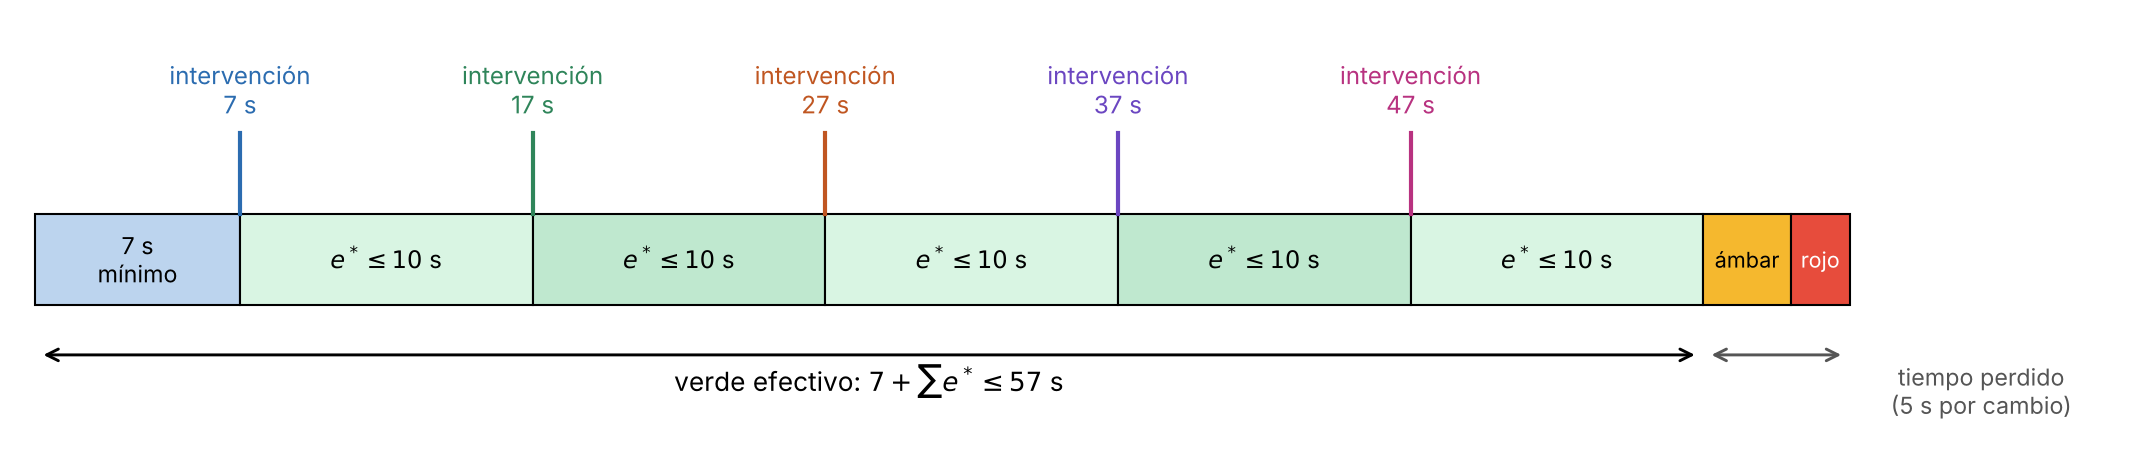
\includegraphics[width=\textwidth]{fig_fase.png}
\caption{Estructura temporal de una fase verde: mínimo de 7\,s, hasta cinco intervenciones con extensiones de hasta 10\,s (verde efectivo máximo de 57\,s) y tiempo perdido de 5\,s por cambio de fase, que el simulador muestra como 3\,s de ámbar y 2\,s de rojo.}
\label{fig:fase}
\end{figure*}

\subsection{Entradas $A$ y $Q$: dos lecturas}
\label{sec:lecturas}
El ejemplo de la Sección~\ref{sec:ejemplo} entrega los vectores ya calculados; el artículo no dice cómo obtener $a_e$ y $q_e$ a lo largo de una simulación. Se implementaron dos lecturas:
\begin{itemize}
\item \textbf{Literal:} $a_e=\beta_e=\sum_{i\le e}x_i$ (arribos acumulados) y $q_e=Q+\sum_{i\le e}x'_i$ con $Q$ la cola total del brazo en rojo (cola prevista, como en el ejemplo).
\item \textbf{Calibrada:} 
\begin{equation}
a_e=\min\bigl(e,\ Q_G+\textstyle\sum_{i\le e}x_i\bigr),\qquad q_e=Q_V,
\label{eq:beta}
\end{equation}
con $Q_G$ la cola del brazo en verde (los vehículos que realmente cruzan están limitados por 1\,veh/s) y $Q_V$ los vehículos llegados al brazo en rojo desde que empezó el verde actual.
\end{itemize}
La lectura calibrada no está respaldada por el texto del artículo: se eligió porque es la única, entre las ocho probadas (Sección~\ref{sec:auditoria}), que reproduce sus resultados. Se presenta, por tanto, como una inferencia por falta de datos. De la ecuación~\eqref{eq:beta}, el factor $\min(e,\cdot)$ se deduce de la saturación de 1\,veh/s, y la elección de $Q_V$ es empírica (Sección~\ref{sec:formulas}); ninguna de las dos partes viene del artículo original.

\subsection{Correcciones de transcripción y de implementación}
La réplica se validó contra las imágenes del artículo original y no contra el texto extraído del PDF ni contra su traducción. Esa comparación detectó los errores de la Tabla~\ref{tab:correcciones}, que se corrigieron antes de obtener los resultados de este trabajo.

\begin{table}[!t]
\caption{Correcciones realizadas al contrastar con el artículo original}
\label{tab:correcciones}
\centering
\footnotesize
\setlength{\tabcolsep}{3pt}
\begin{tabular}{@{}p{0.33\columnwidth}p{0.58\columnwidth}@{}}
\toprule
Elemento & Corrección \\
\midrule
Operador \emph{mt} (Tabla~V) & Vale 0 para $x\le x_0$; antes devolvía $\mu_A$ \\
Conjunto \emph{very long} de colas (Tabla~IV) & Pico en $q=28$ (antes 29); también \emph{lt}(very long) \\
Reglas de 27, 37 y 47\,s & 25 reglas, cinco por intervención, leídas de la imagen (antes 24 reglas copiadas del texto extraído, que mezcla las dos columnas) \\
Momento de intervención & Tras 7\,s de verde y máximo 57\,s (antes 8\,s y 58\,s) \\
Último segundo del verde difuso & Se reprocesaba y contaba dos veces sus arribos (6\,\% a 12\,\% más vehículos que los generados) \\
Verdes del ciclo fijo y Tabla~I & Verdes enteros y fórmula de Webster completa \\
\bottomrule
\end{tabular}
\fuente{comparación propia entre la primera versión del código y las imágenes de las páginas del artículo original: Tablas~V y~VI (p.~712), Tabla~IV (p.~711), Apéndice (pp.~715 y~716) y estructura temporal (p.~709); verificada con \texttt{test\_paper\_tables.py}.}
\end{table}

\subsection{Implementación y visualización}
El código (Python, \texttt{numpy} y \texttt{matplotlib}) contiene el modelo, el controlador, un motor paso a paso con equivalencia comprobada frente a la simulación por lotes, y un simulador gráfico. La Fig.~\ref{fig:simulador} muestra la ventana completa durante una simulación; sus apartados se presentan por separado en las Figs.~\ref{fig:sim-calle} a~\ref{fig:sim-registro}. Todas las figuras corresponden al mismo instante (720/2160\,veh/h, semilla 1, $t=118$\,s), en el que el controlador decide extender el verde del brazo E-W en 4\,s por la regla R2 de la intervención de 47\,s.

\begin{figure*}[!t]
\centering
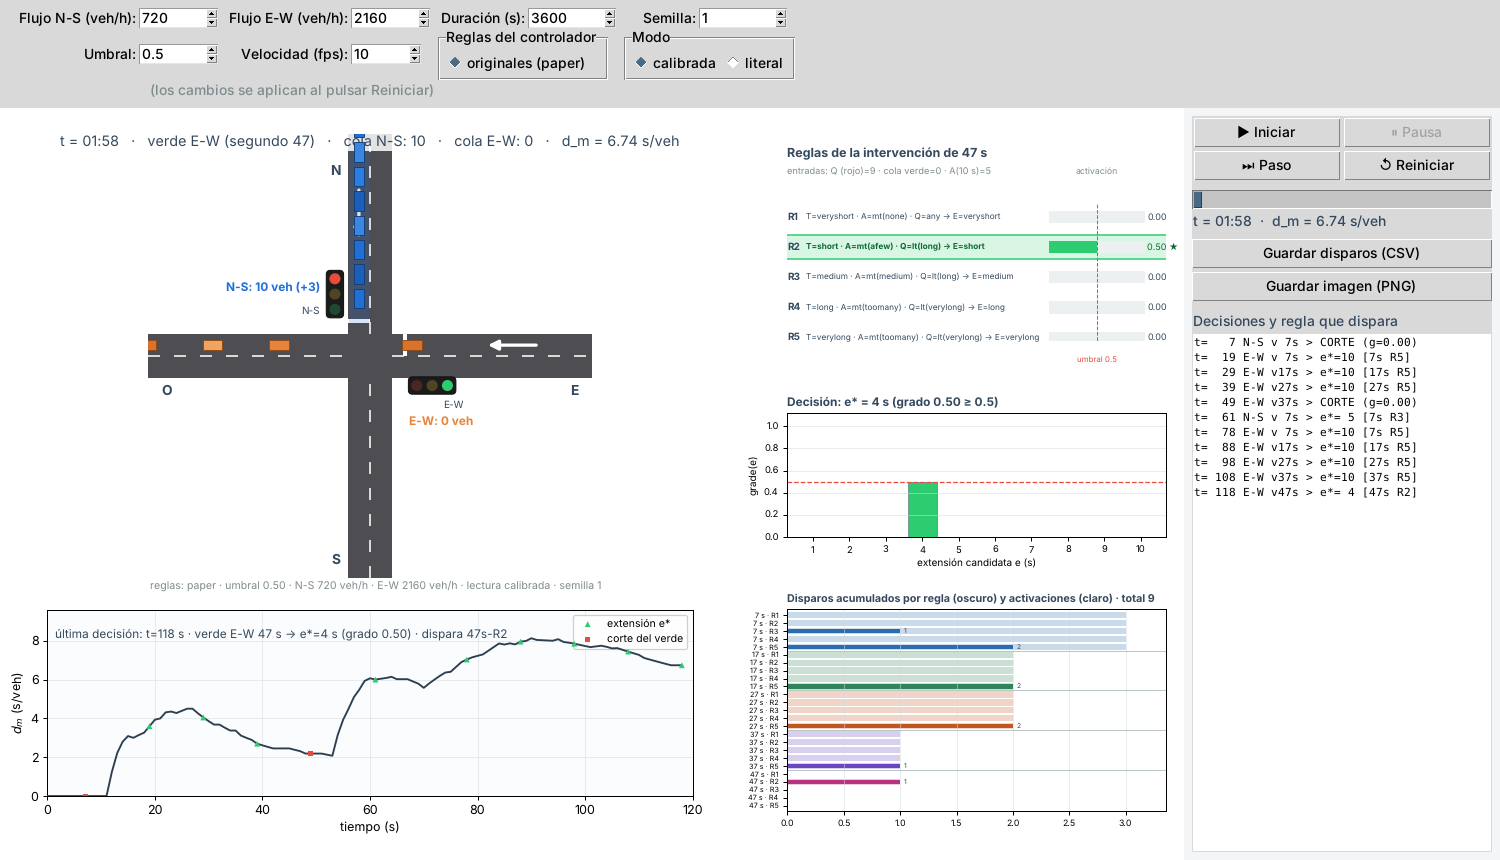
\includegraphics[width=\textwidth]{fig_simulador.png}
\caption{Captura de la ventana del simulador: barra de parámetros (flujos, duración, semilla, umbral, velocidad, reglas y modo), calle, panel de reglas de la intervención, vector de grados, disparos acumulados, retardo medio $d_m$ y, a la derecha, los botones de control y el registro de decisiones.}
\label{fig:simulador}
\end{figure*}

\subsection{Apartados del simulador}
\label{sec:apartados}
\textit{La calle} (Fig.~\ref{fig:sim-calle}) representa el cruce de las dos calles unidireccionales. Los vehículos azules circulan por la calle N-S y los naranjas por la E-W; avanzan, frenan en rojo y arrancan en verde, y cada brazo tiene un semáforo de tres luces. El ámbar y el despeje corresponden a los 5\,s de tiempo perdido por cambio de fase (3\,s de ámbar y 2\,s de despeje) y no alteran el modelo numérico. El encabezado indica el tiempo, el brazo en verde, las colas y el retardo medio $d_m$; el número entre paréntesis en la etiqueta de cada brazo cuenta los vehículos en cola que no caben en el dibujo, que solo muestra siete.

\textit{El panel de reglas} (Fig.~\ref{fig:sim-reglas}) lista las cinco reglas de la intervención vigente, con las entradas de esa decisión (cola del brazo en rojo, cola del brazo en verde y arribos esperados) y una barra con la activación de cada regla. La regla que dispara se resalta con $\star$.

\textit{El vector de grados} (Fig.~\ref{fig:sim-decision}) muestra el grado $g(e)$ de cada extensión candidata de 1 a 10\,s, la línea del umbral 0.5 y la extensión elegida en verde. Si ningún grado alcanza el umbral, el controlador corta el verde.

\textit{Los disparos acumulados} (Fig.~\ref{fig:sim-disparos}) muestran, para cada una de las 25 reglas, cuántas veces se activó (barra clara) y cuántas veces decidió (barra oscura).

\textit{La traza del retardo} (Fig.~\ref{fig:sim-traza}) registra $d_m$ en el tiempo, con una marca por cada extensión y por cada corte. Por último, \textit{el registro de decisiones} (Fig.~\ref{fig:sim-registro}) resume cada decisión en una línea: el tiempo, el brazo, el segundo de verde, la extensión elegida y la regla que dispara. La ventana permite además guardar los disparos en un archivo CSV y la imagen en PNG.

\begin{figure*}[!t]
\centering
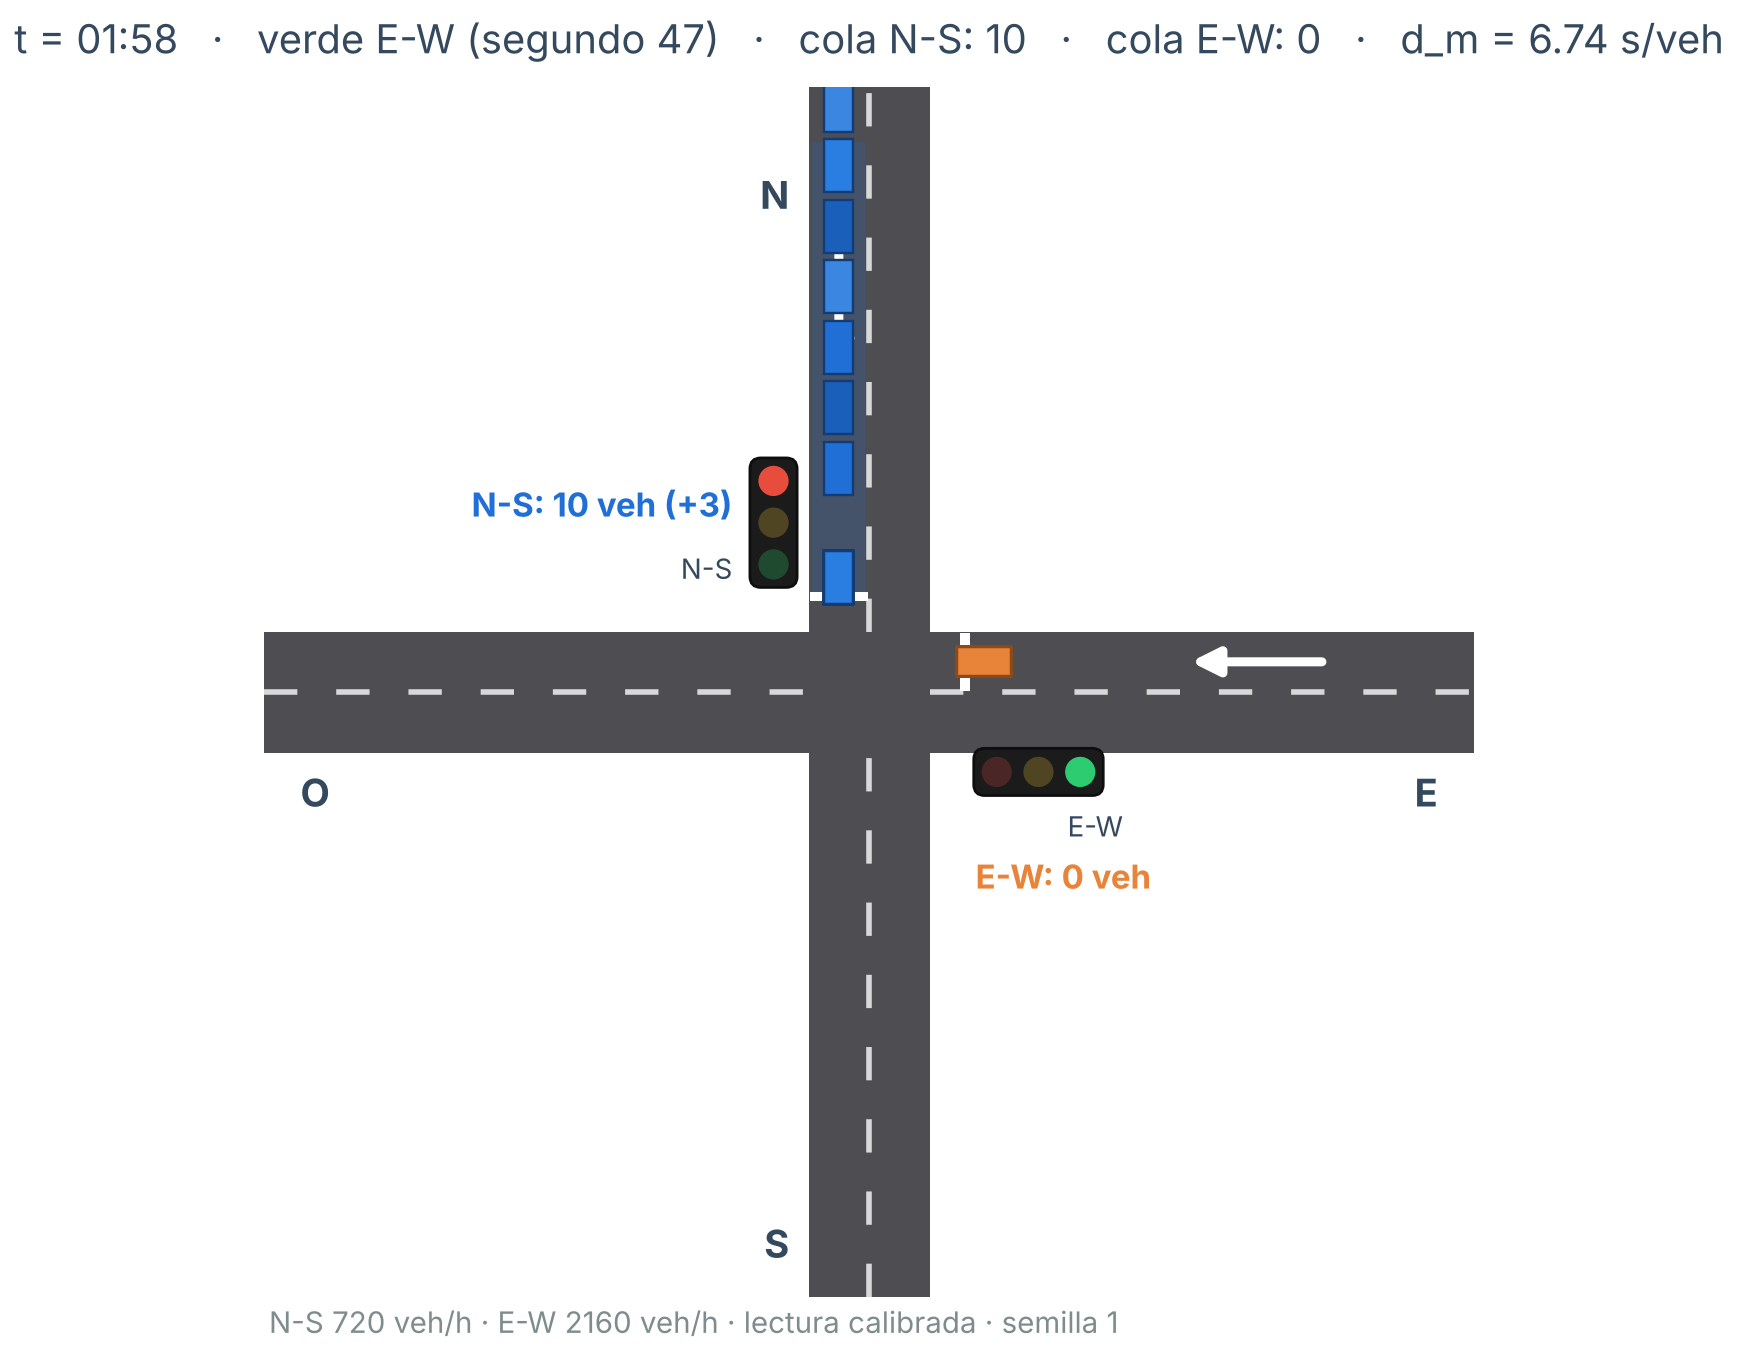
\includegraphics[width=0.62\textwidth]{fig_sim_calle.png}
\caption{La calle: cruce con vehículos en movimiento (azul: N-S; naranja: E-W), semáforos de tres luces, colas y encabezado con el tiempo y $d_m$.}
\label{fig:sim-calle}
\end{figure*}

\begin{figure*}[!t]
\centering
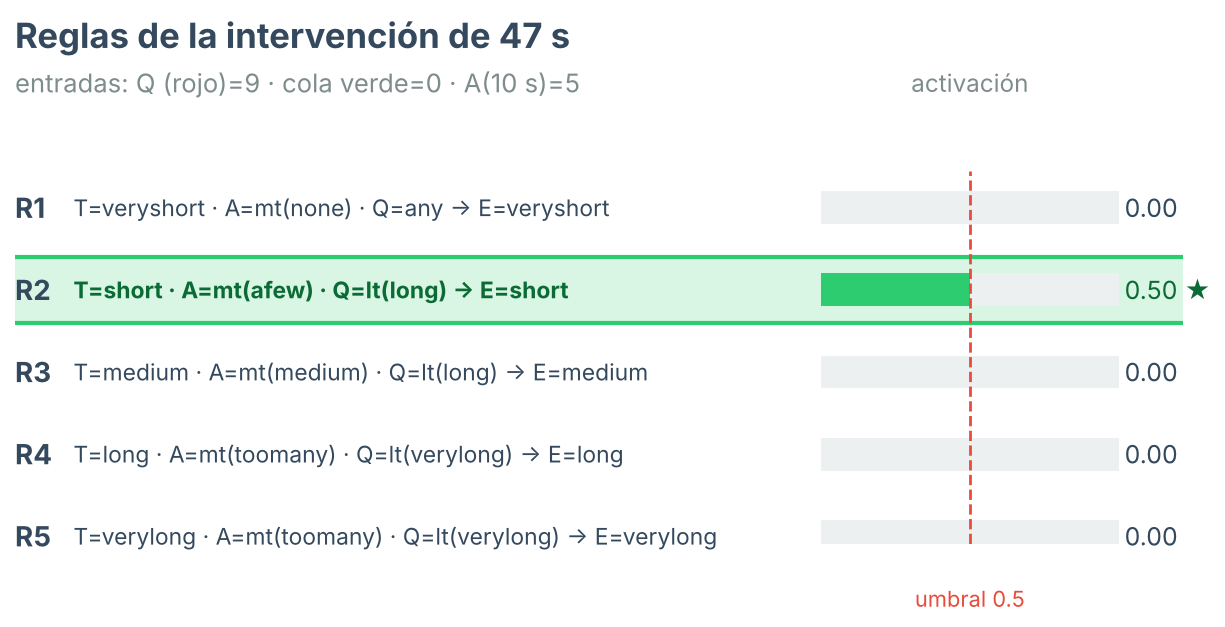
\includegraphics[width=0.62\textwidth]{fig_sim_reglas.png}
\caption{Panel de reglas de la intervención de 47\,s: entradas de la decisión, activación de cada regla y regla que dispara ($\star$, R2).}
\label{fig:sim-reglas}
\end{figure*}

\begin{figure*}[!t]
\centering
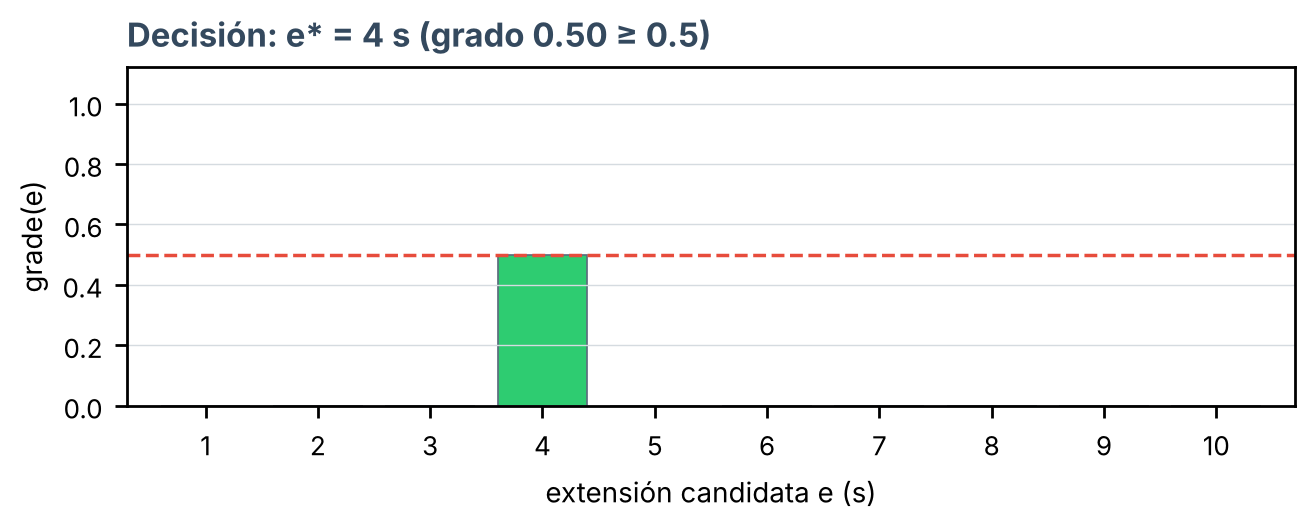
\includegraphics[width=0.62\textwidth]{fig_sim_decision.png}
\caption{Vector de grados $g(e)$ de las extensiones candidatas, umbral 0.5 y extensión elegida ($e^*=4$\,s, grado 0.50).}
\label{fig:sim-decision}
\end{figure*}

\begin{figure*}[!t]
\centering
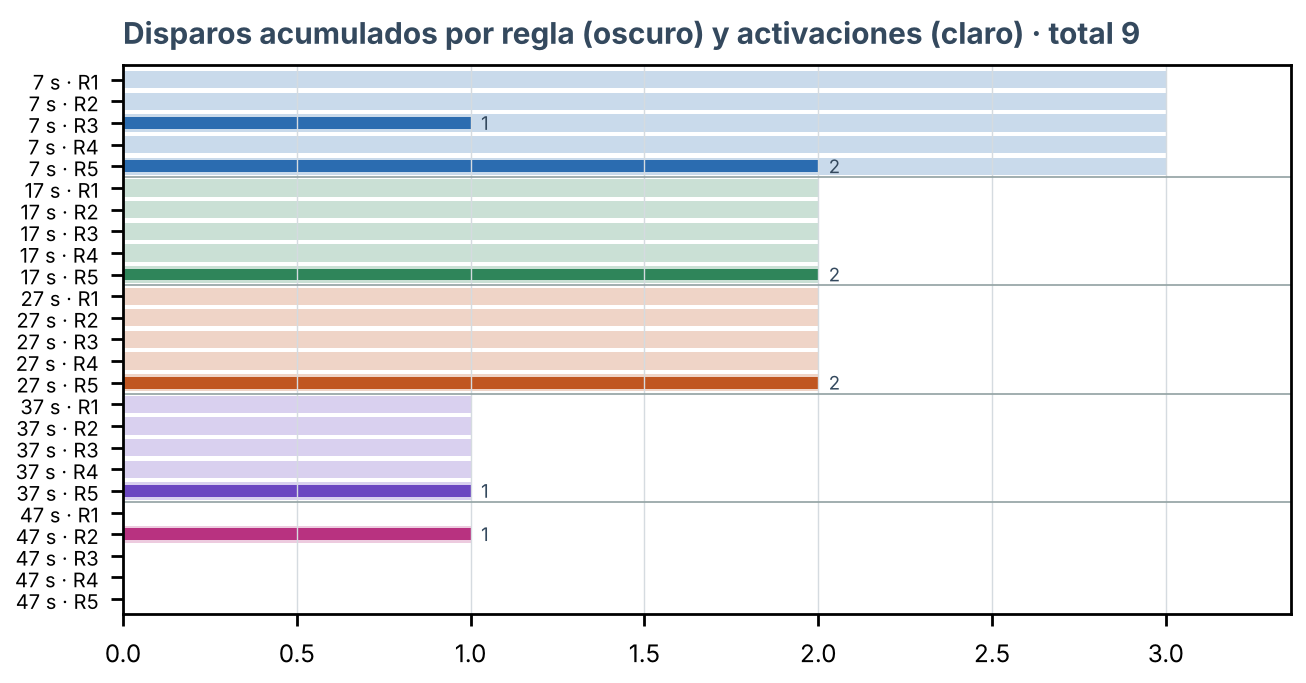
\includegraphics[width=0.62\textwidth]{fig_sim_disparos.png}
\caption{Disparos acumulados (barra oscura) y activaciones (barra clara) de las 25 reglas, agrupadas por intervención, hasta $t=118$\,s.}
\label{fig:sim-disparos}
\end{figure*}

\begin{figure*}[!t]
\centering
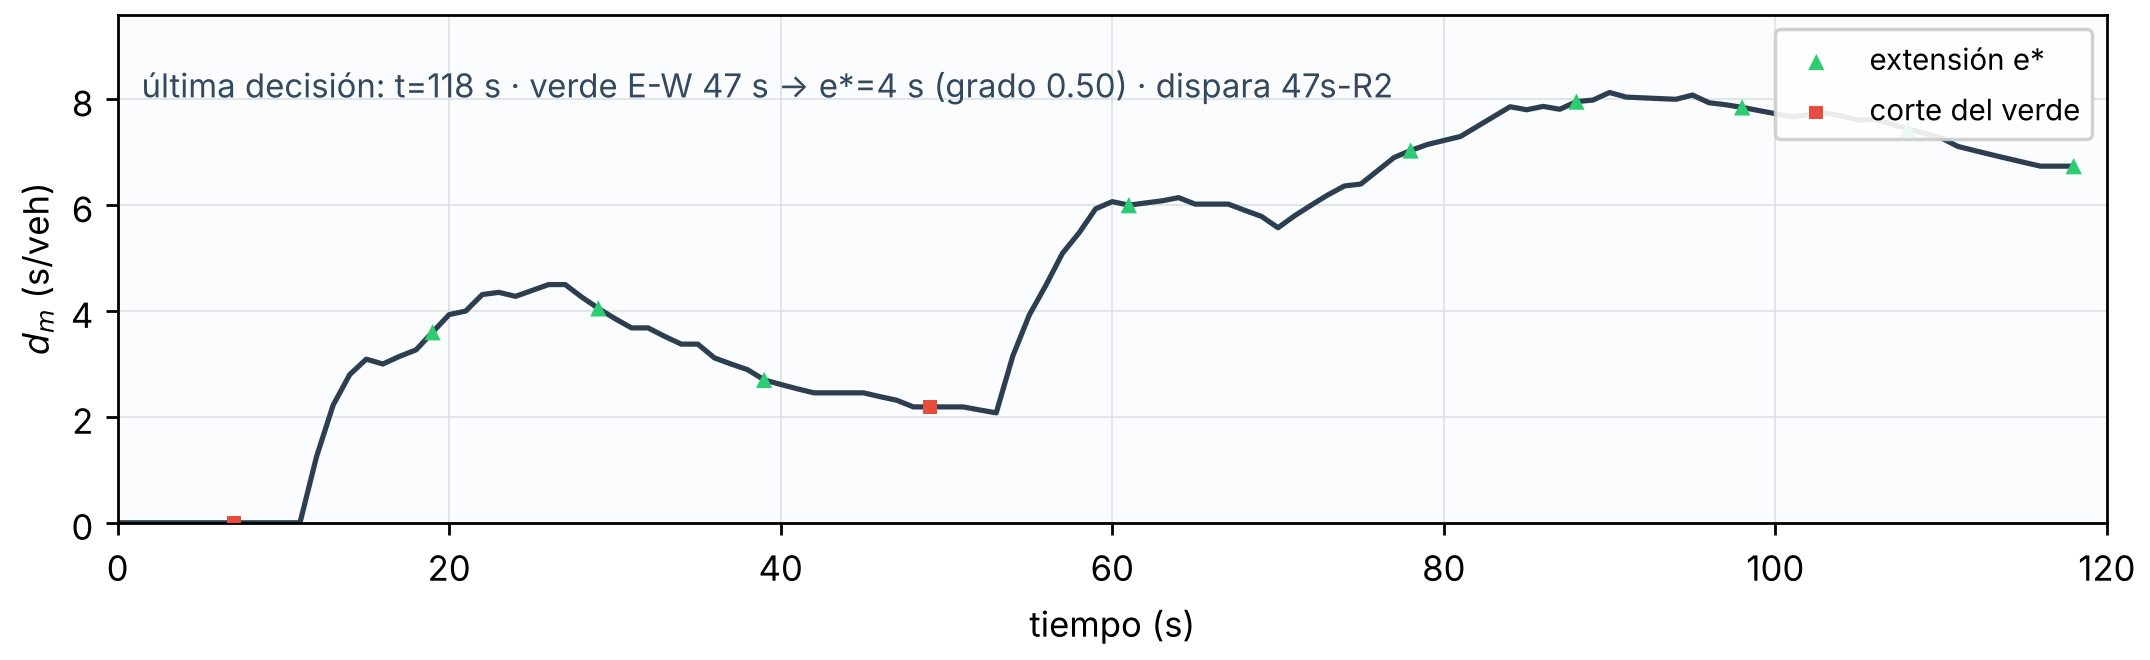
\includegraphics[width=0.9\textwidth]{fig_sim_traza.png}
\caption{Traza del retardo medio $d_m$ en el tiempo. Los triángulos verdes marcan las extensiones del verde y los cuadrados rojos, los cortes.}
\label{fig:sim-traza}
\end{figure*}

\begin{figure}[!t]
\centering
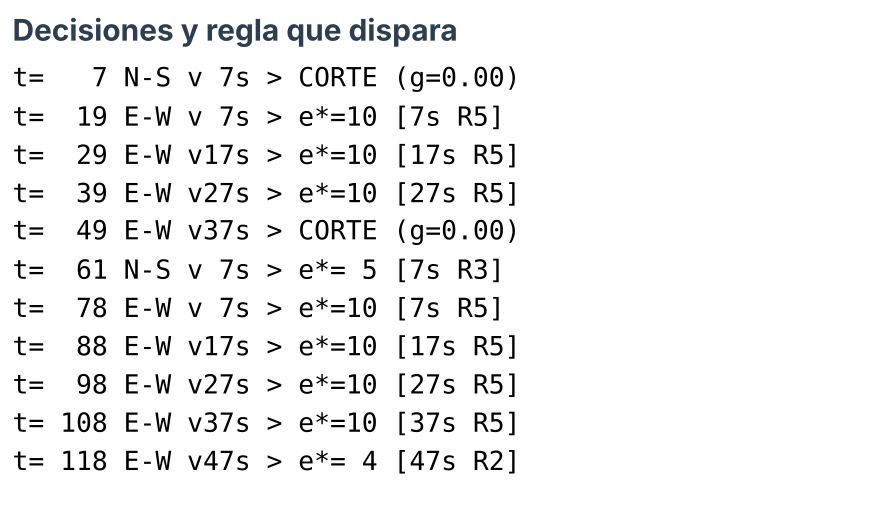
\includegraphics[width=\columnwidth]{fig_sim_registro.png}
\caption{Registro de decisiones del simulador: tiempo, brazo en verde, segundo de verde, extensión elegida y regla que dispara.}
\label{fig:sim-registro}
\end{figure}

% =============================================================================
\section{Metodología de validación}
\label{sec:metodologia}

\subsection{Verificación contra lo impreso}
Un conjunto de 42 comprobaciones automáticas compara el código con los valores impresos en el artículo: los conjuntos de las Tablas~II a~IV, los operadores de las Tablas~V y~VI, las 25 reglas, cada fila de la Tabla~VII del ejemplo, la regla de empate y de umbral, y la estructura temporal (intervenciones a 7, 17, 27, 37 y 47\,s, verde máximo de 57\,s). Otras comprobaciones verifican que el motor paso a paso devuelve el mismo $d_m$ que la simulación por lotes, y que lo mostrado en el panel de reglas (activaciones, regla que dispara, extensión elegida) coincide con lo calculado por el controlador.

\subsection{Protocolo estadístico}
Cada combinación de caudal se simula durante 7200\,s, como en el artículo, con 20 réplicas independientes y semilla base 0; el controlador difuso usa semillas distintas de las del ciclo fijo. Las 16 combinaciones son las de las Tablas~I y~VIII. El artículo solo indica «muchas corridas»; el número de réplicas es, por tanto, una decisión de la réplica. Para cada celda se calcula el intervalo de confianza (IC) al 95\,\% de la media con la distribución $t$ de Student ($n=20$). La mejora del difuso sobre el ciclo fijo se contrasta con la prueba de Welch, porque ambos controladores no comparten llegadas; el sesgo entre la réplica y lo publicado se resume con la media de los errores relativos de las 16 celdas, su IC 95\,\%, una prueba $t$ de una muestra y una prueba de signos exacta. Como el artículo publica solo una cifra por celda, sin dispersión, la condición «el valor publicado cae dentro del IC de la réplica» es exigente y se usa como una medida adicional, no como criterio de aceptación.

\subsection{Métricas}
Para cada tabla se reportan el error relativo de cada celda, su media y su máximo, y para el controlador difuso el número de combinaciones en que mejora a la línea base (el artículo reporta 16 de 16). La mejora porcentual se calcula respecto del ciclo fijo simulado.

\subsection{Auditoría de las lecturas de $A$ y $Q$}
\label{sec:auditoria-met}
Con las reglas fijas se probaron las ocho combinaciones de: arribos (acumulados o cruces limitados por la saturación), valor en que se evalúa $Q$ (cola predicha o actual) y definición de la cola (total, o llegados desde el inicio del verde), y se midió el error frente a la Tabla~VIII (10 réplicas de 7200\,s).

\subsection{Pruebas complementarias}
Dos experimentos adicionales aportan evidencia sobre el modelo, sin modificar la réplica: la comparación entre llegadas aleatorias y llegadas fijas (un vehículo cada $1/\lambda$ segundos con desfase aleatorio), y un experimento exploratorio de reducción de reglas que conserva las reglas del artículo y quita algunas (Sección~\ref{sec:reglas-disparos}).

% =============================================================================
\section{Resultados}
\label{sec:resultados}

\subsection{Fuzzificación}
La Fig.~\ref{fig:validacion} superpone los valores impresos en el artículo sobre las curvas del código para las Tablas~II, IV, V y~VI. La diferencia máxima es 0.000 en los cuatro paneles: los conjuntos y los operadores \emph{mt} y \emph{lt} del código son exactamente los del artículo.

\begin{figure*}[!t]
\centering
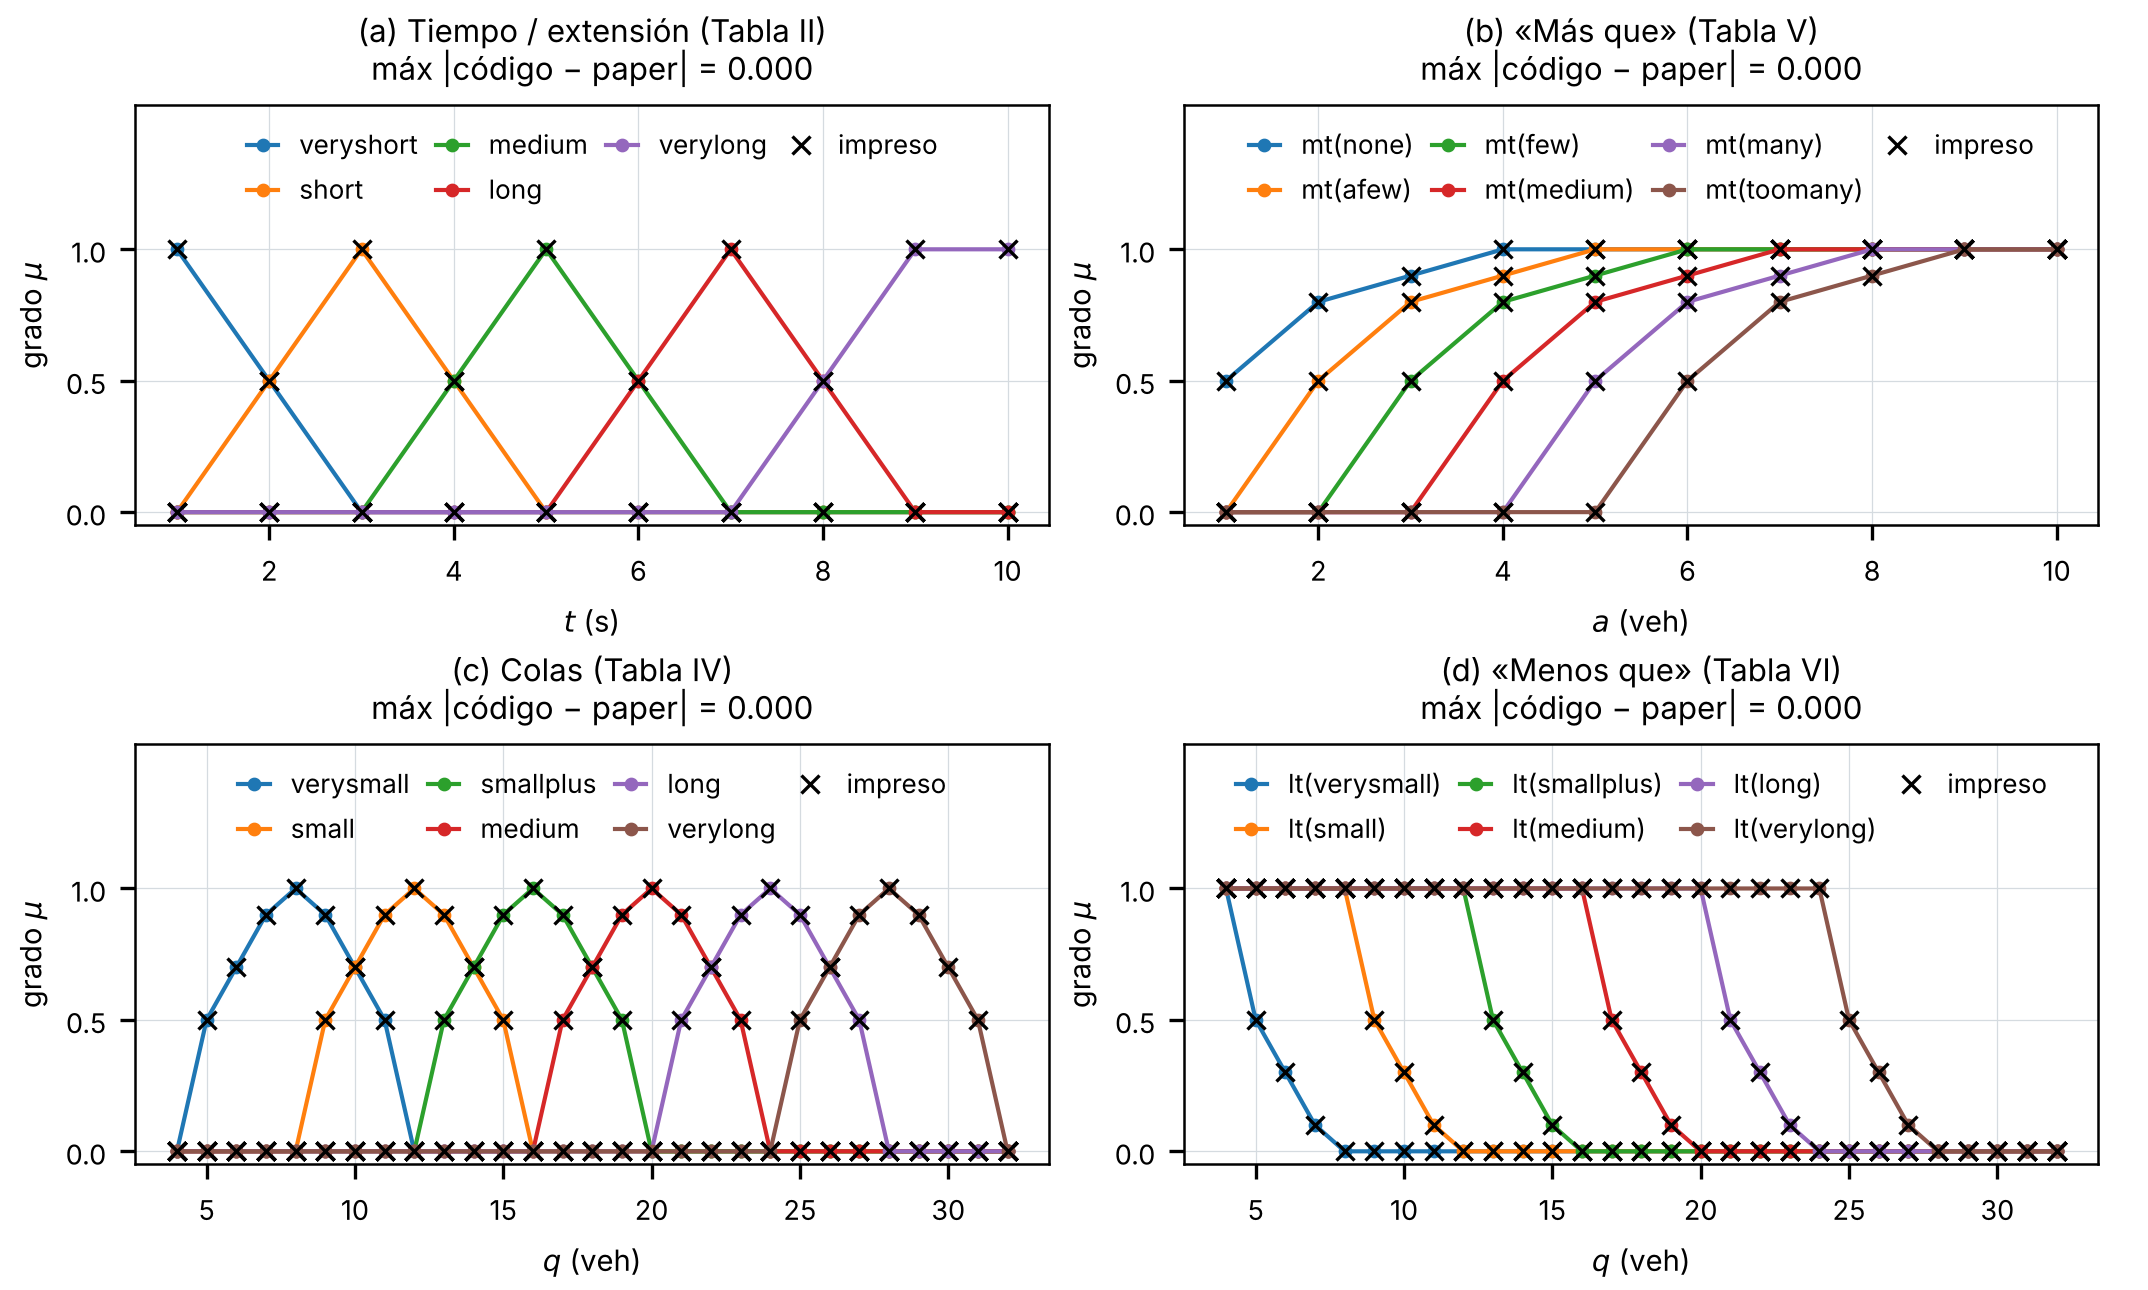
\includegraphics[width=\textwidth]{fig_validacion_curvas.png}
\caption{Validación de la fuzzificación: curvas del código (líneas) y valores impresos en el artículo original ($\times$). Los marcadores coinciden con las curvas en todos los puntos.}
\label{fig:validacion}
\end{figure*}

\subsection{Ejemplo trabajado}
Con las entradas del ejemplo, el controlador reproduce cada fila de la Tabla~VII del artículo (las cinco reglas y la fila final) y selecciona $e^*=10$\,s (Fig.~\ref{fig:tabla7}). Las comprobaciones se hicieron con la lectura del ejemplo (arribos acumulados y cola prevista).

\subsection{Tabla I: validación del modelo}
La simulación de ciclo fijo reproduce la columna «Model» con un error relativo medio de 2.1\,\% y la fórmula de Webster reproduce la columna «Formula» con 0.8\,\% (Tabla~\ref{tab:tablaI}). La mayor desviación, $-7.9$\,\% en 360/2160, se debe a que el verde de 8.1\,s se redondea a 8\,s. Las Tablas~I y~VIII del artículo se comparan en la Fig.~\ref{fig:dispersion}.

\begin{table}[!t]
\caption{Tabla I del artículo original: retardo medio (s/veh) del ciclo fijo con ajustes óptimos. Simulación (20 réplicas de 7200\,s) y fórmula de Webster frente a los valores publicados.}
\label{tab:tablaI}
\centering
\scriptsize
\setlength{\tabcolsep}{2.6pt}
\begin{tabular}{@{}lrrrrrr@{}}
\toprule
N--S/E--W & Sim. & Paper & Err.\,\% & Fórm. & Paper & Err.\,\% \\
\midrule
360/360 & 7.29 & 7.2 & +1.2 & 7.45 & 7.4 & +0.7 \\
360/720 & 7.48 & 7.4 & +1.1 & 7.95 & 7.9 & +0.6 \\
360/1080 & 7.76 & 7.9 & -1.8 & 8.34 & 8.4 & -0.8 \\
360/1440 & 8.24 & 8.4 & -1.9 & 9.04 & 9.0 & +0.4 \\
360/1800 & 9.19 & 9.3 & -1.2 & 10.31 & 10.2 & +1.1 \\
360/2160 & 11.33 & 12.3 & -7.9 & 12.72 & 12.9 & -1.4 \\
360/2520 & 16.17 & 15.8 & +2.3 & 17.99 & 18.9 & -4.8 \\
720/720 & 9.36 & 9.7 & -3.5 & 9.96 & 10.0 & -0.4 \\
720/1080 & 10.63 & 10.8 & -1.6 & 11.59 & 11.6 & -0.1 \\
720/1440 & 12.49 & 12.7 & -1.6 & 13.74 & 13.8 & -0.4 \\
720/1800 & 15.35 & 15.9 & -3.5 & 17.36 & 17.3 & +0.3 \\
720/2160 & 21.21 & 21.8 & -2.7 & 24.96 & 24.9 & +0.2 \\
1080/1080 & 13.53 & 13.6 & -0.5 & 14.92 & 14.9 & +0.1 \\
1080/1440 & 17.77 & 17.9 & -0.7 & 19.76 & 19.7 & +0.3 \\
1080/1800 & 25.54 & 25.8 & -1.0 & 29.27 & 29.2 & +0.3 \\
1440/1440 & 26.86 & 27.3 & -1.6 & 30.73 & 30.7 & +0.1 \\
\midrule
\multicolumn{3}{@{}l}{Error relativo medio} & 2.1 & & & 0.8 \\
\bottomrule
\end{tabular}
\fuente{columnas «Paper»: Tabla~I del artículo original (p.~708); «Sim.»: simulación propia con las ecuaciones \eqref{eq:colaR}--\eqref{eq:dm} (\texttt{run\_experiments.py}, \texttt{resultados/resultados\_oficiales.json}); «Fórm.»: evaluación de \eqref{eq:retardo-webster} con los ajustes de \eqref{eq:webster}. Err.\,$=100\,(\text{réplica}-\text{paper})/\text{paper}$.}
\end{table}


\begin{figure*}[!t]
\centering
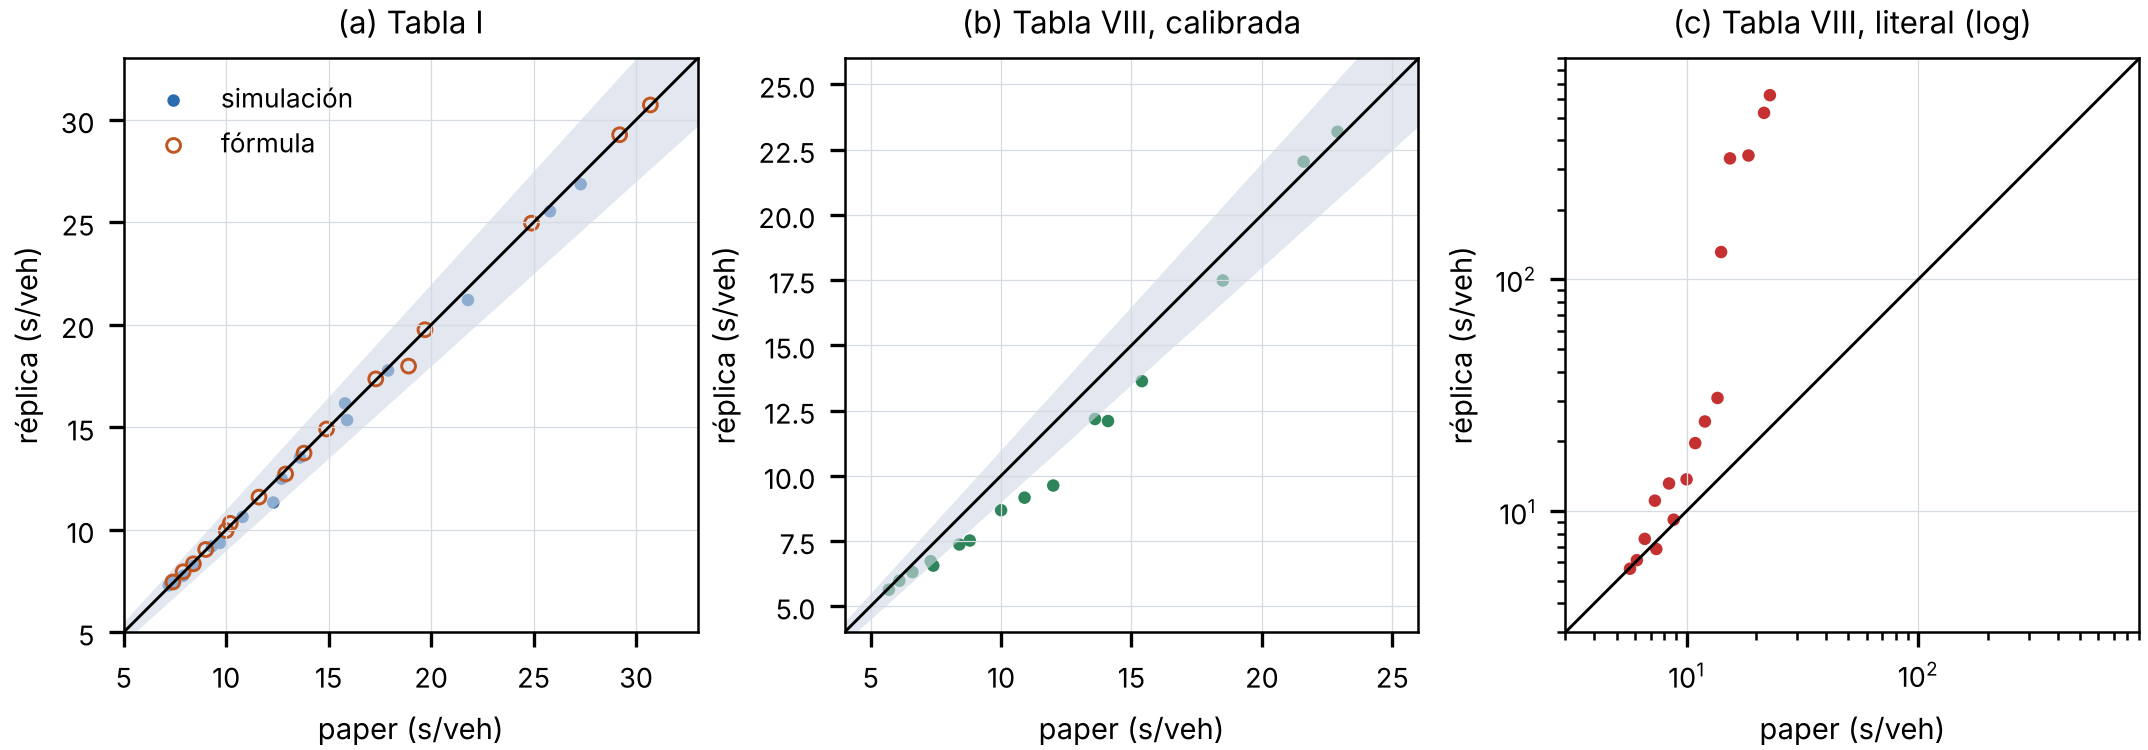
\includegraphics[width=\textwidth]{fig_dispersion.png}
\caption{Réplica frente al artículo original (la diagonal es la coincidencia exacta; la banda es $\pm 10$\,\%): (a) Tabla~I; (b) Tabla~VIII con la lectura calibrada; (c) Tabla~VIII con la lectura literal, en escala logarítmica.}
\label{fig:dispersion}
\end{figure*}

\subsection{Tabla VIII: controlador difuso frente al ciclo fijo}
Con la lectura calibrada, el controlador difuso mejora al ciclo fijo en las 16 combinaciones, con mejoras entre 14\,\% y 30\,\% (el artículo imprime entre +10\,\% y +21\,\%; recalculadas con los retardos impresos, entre 9.7\,\% y 23.7\,\%, pues en la celda 720/720 imprime +21\,\% y sus retardos de 9.7 y 7.4\,s dan 23.7\,\%). El error relativo frente a los retardos publicados es 9.3\,\% en promedio y 19.8\,\% como máximo; en los caudales altos (1080/1800 y 1440/1440) la diferencia es de $\pm$2\,\%, mientras que en caudales medios el difuso simulado queda entre 10\,\% y 20\,\% por debajo del publicado (Tabla~\ref{tab:tabla8} y Fig.~\ref{fig:tabla8}). Con la lectura literal, solo 5 de 16 combinaciones mejoran al ciclo fijo y el sistema se satura desde 360/1440; en 1440/1440 el retardo supera 600\,s.

\begin{table*}[!t]
\caption{Difuso frente al ciclo fijo (Tabla VIII del original) y a un controlador actuado por detector (comparador adicional); 20 réplicas de 7200\,s con números aleatorios comunes. Retardo medio (s/veh) $\pm$ semiancho del IC 95\,\%. «Mej.»: reducción del difuso respecto del fijo (\%), con la réplica y con los retardos impresos; «Dif. vs act.»: diferencia relativa del difuso respecto del actuado; $^{*}$: significativa (Wilcoxon pareado, Holm, $p<0.05$).}
\label{tab:tabla8}
\centering
\footnotesize
\setlength{\tabcolsep}{3.2pt}
\begin{tabular}{@{}lrrrrrrrrr@{}}
\toprule
 & \multicolumn{2}{c}{Ciclo fijo} & \multicolumn{3}{c}{Difuso (25 reglas, calibrada)} & \multicolumn{2}{c}{Mej.\,(\%)} & Accionado & Dif. vs \\
\cmidrule(lr){2-3}\cmidrule(lr){4-6}\cmidrule(lr){7-8}
N--S/E--W & Réplica & Pub. & Réplica & Pub. & Err.\,\% & Réplica & Pub. & (s/veh) & act.\,\% \\
\midrule
360/360 & 7.29\,$\pm$\,0.08 & 7.2 & 5.58\,$\pm$\,0.07 & 5.7 & -2.2 & 23.5 & 20.8 & 6.55 & -14.8$^{*}$ \\
360/720 & 7.48\,$\pm$\,0.07 & 7.4 & 5.96\,$\pm$\,0.05 & 6.1 & -2.2 & 20.3 & 17.6 & 7.18 & -16.9$^{*}$ \\
360/1080 & 7.76\,$\pm$\,0.11 & 7.9 & 6.25\,$\pm$\,0.05 & 6.6 & -5.4 & 19.5 & 16.5 & 7.86 & -20.5$^{*}$ \\
360/1440 & 8.24\,$\pm$\,0.15 & 8.4 & 6.69\,$\pm$\,0.05 & 7.3 & -8.4 & 18.9 & 13.1 & 8.59 & -22.2$^{*}$ \\
360/1800 & 9.19\,$\pm$\,0.12 & 9.3 & 7.39\,$\pm$\,0.11 & 8.4 & -12.0 & 19.5 & 9.7 & 9.35 & -20.9$^{*}$ \\
360/2160 & 11.33\,$\pm$\,0.62 & 12.3 & 8.69\,$\pm$\,0.14 & 10.0 & -13.1 & 23.2 & 18.7 & 10.14 & -14.3$^{*}$ \\
360/2520 & 16.17\,$\pm$\,2.11 & 15.8 & 12.00\,$\pm$\,0.34 & 13.6 & -11.7 & 25.8 & 13.9 & 11.95 & +0.4 \\
720/720 & 9.36\,$\pm$\,0.07 & 9.7 & 6.57\,$\pm$\,0.07 & 7.4 & -11.3 & 29.8 & 23.7 & 8.11 & -19.0$^{*}$ \\
720/1080 & 10.63\,$\pm$\,0.10 & 10.8 & 7.53\,$\pm$\,0.07 & 8.8 & -14.4 & 29.2 & 18.5 & 9.04 & -16.7$^{*}$ \\
720/1440 & 12.49\,$\pm$\,0.20 & 12.7 & 9.33\,$\pm$\,0.14 & 10.9 & -14.4 & 25.3 & 14.2 & 10.20 & -8.5$^{*}$ \\
720/1800 & 15.35\,$\pm$\,0.22 & 15.9 & 12.19\,$\pm$\,0.24 & 14.1 & -13.5 & 20.6 & 11.3 & 11.81 & +3.2$^{*}$ \\
720/2160 & 21.21\,$\pm$\,0.36 & 21.8 & 17.64\,$\pm$\,0.64 & 18.5 & -4.6 & 16.8 & 15.1 & 14.94 & +18.1$^{*}$ \\
1080/1080 & 13.53\,$\pm$\,0.13 & 13.6 & 9.76\,$\pm$\,0.14 & 12.0 & -18.6 & 27.8 & 11.8 & 10.35 & -5.6$^{*}$ \\
1080/1440 & 17.77\,$\pm$\,0.20 & 17.9 & 13.79\,$\pm$\,0.25 & 15.4 & -10.4 & 22.4 & 14.0 & 12.67 & +8.9$^{*}$ \\
1080/1800 & 25.54\,$\pm$\,0.41 & 25.8 & 22.34\,$\pm$\,0.91 & 21.6 & +3.4 & 12.5 & 16.3 & 17.27 & +29.4$^{*}$ \\
1440/1440 & 26.86\,$\pm$\,0.47 & 27.3 & 23.17\,$\pm$\,0.90 & 22.9 & +1.2 & 13.8 & 16.1 & 18.01 & +28.7$^{*}$ \\
\midrule
\multicolumn{5}{@{}l}{Mejora al ciclo fijo: 16/16 (Holm $p\le$ 3.1e-05)} & 9.2 (media) & \multicolumn{4}{l}{error máx. 18.6\,\%} \\
\multicolumn{5}{@{}l}{Medias de los 16 flujos (s/veh): fijo / difuso / accionado} & \multicolumn{5}{l}{13.76 / 10.93 / 10.88} \\
\bottomrule
\end{tabular}
\fuente{columnas «Pub.»: Tabla~VIII del artículo original (p.~715); «Mej. pub.» recalculada con sus retardos (el artículo imprime +21\,\% en 720/720; recalculado, 23.7\,\%). Réplica: \texttt{analisis\_estadistico.py} y \texttt{comparadores.py}; IC con la distribución $t$ de Student, $n_r=20$. El comparador accionado (extensión por hueco de 3\,s, verde de 7 a 57\,s) no es parte del artículo original.}
\end{table*}


La Fig.~\ref{fig:mejora} compara la mejora porcentual sobre el ciclo fijo. La mejora de la réplica es mayor que la publicada en los caudales medios, y de orden comparable en los altos.

\begin{figure}[!t]
\centering
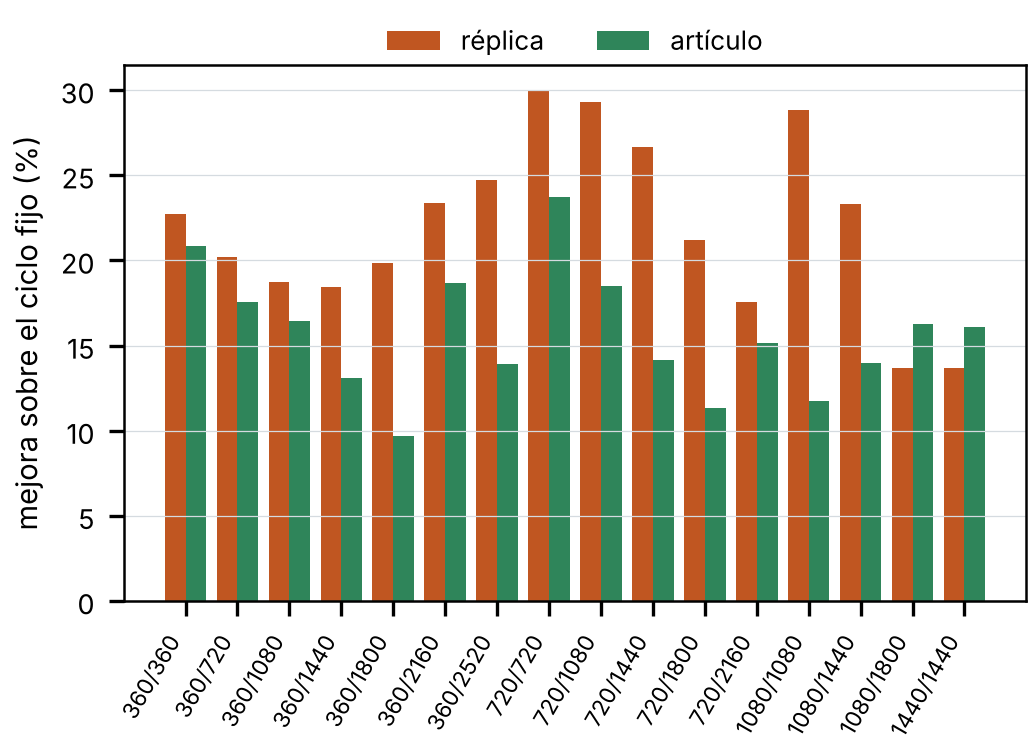
\includegraphics[width=\columnwidth]{fig_mejora.png}
\caption{Mejora porcentual del controlador difuso sobre el ciclo fijo, en la réplica y en el artículo original. Fuente: la mejora del artículo se recalcula como (fijo $-$ difuso)/fijo con los retardos impresos en su Tabla~VIII (p.~715).}
\label{fig:mejora}
\end{figure}

\begin{figure*}[!t]
\centering
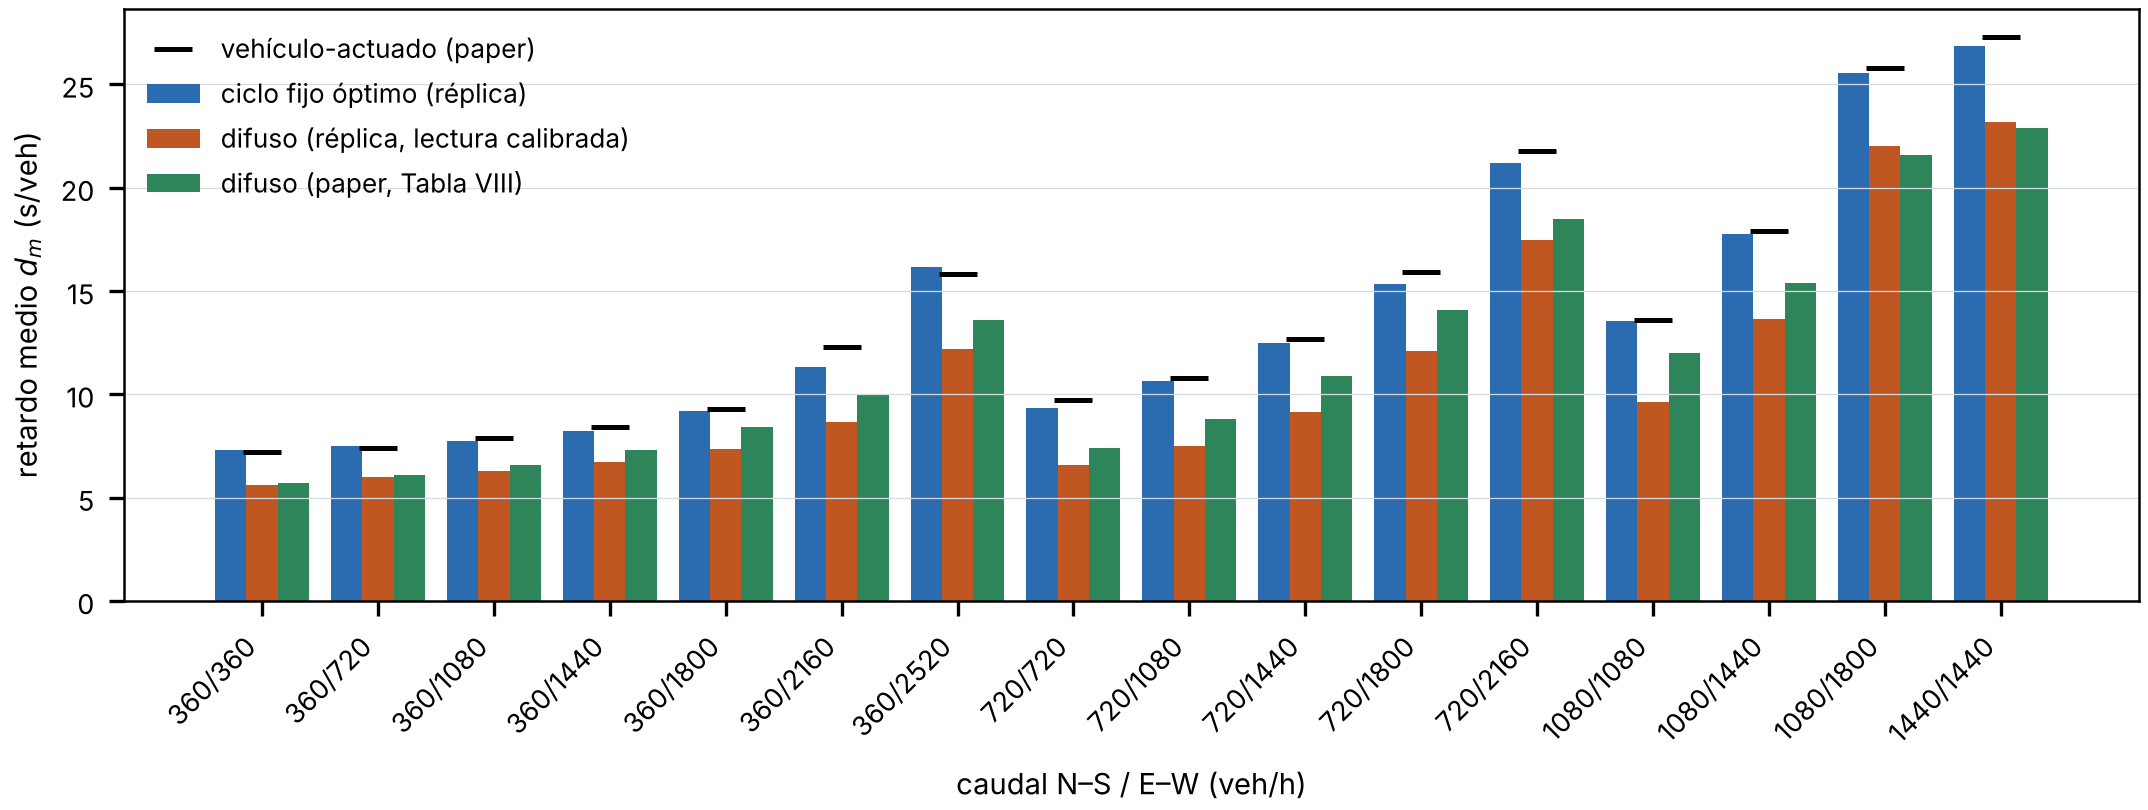
\includegraphics[width=0.92\textwidth]{fig_tabla8.png}
\caption{Retardo medio de la réplica y del artículo original en las 16 combinaciones de caudal.}
\label{fig:tabla8}
\end{figure*}

\subsection{Incertidumbre estadística y sesgo}
\label{sec:estadistica}
La Tabla~\ref{tab:estadistica} y la Fig.~\ref{fig:incertidumbre} añaden los intervalos de confianza de cada celda. Tres resultados se desprenden de ellas.

\textit{Primero}, la mejora del difuso sobre el ciclo fijo es estadísticamente clara: la prueba de Welch da $p<0.001$ en las 16 combinaciones. Este es el resultado cualitativo central del artículo original y se reproduce sin ambigüedad.

\textit{Segundo}, el ciclo fijo se reproduce con un sesgo pequeño: el error medio respecto de lo publicado es $-1.6$\,\% (IC 95\,\% de $-2.8$ a $-0.3$), y el valor publicado cae dentro del IC de la réplica en 6 de 16 celdas. El sesgo es estadísticamente distinto de cero (prueba de signos, $p=0.02$), pero su magnitud es mucho menor que la diferencia entre controladores.

\textit{Tercero}, el controlador difuso muestra un sesgo mayor y sistemático: el error medio es $-8.8$\,\% (IC 95\,\% de $-12.3$ a $-5.4$; 14 de 16 celdas negativas, prueba de signos $p=0.004$), y el valor publicado cae dentro del IC solo en 3 de 16 celdas (360/360, 1080/1800 y 1440/1440). En consecuencia, el controlador de esta réplica produce retardos algo menores que los publicados, y su mejora sobre el ciclo fijo (14\,\% a 30\,\%) es mayor que la publicada (10\,\% a 21\,\% impresa). La réplica de la mejora cualitativa es sólida; la réplica de la magnitud, no. Una posible causa es el punto abierto de la Sección~\ref{sec:lecturas}: el modo de medir $A$ y $Q$ no está especificado, y la lectura elegida reproduce la tendencia pero no el nivel exacto. Esta interpretación es una hipótesis y no se probó con datos adicionales.

\begin{figure}[!t]
\centering
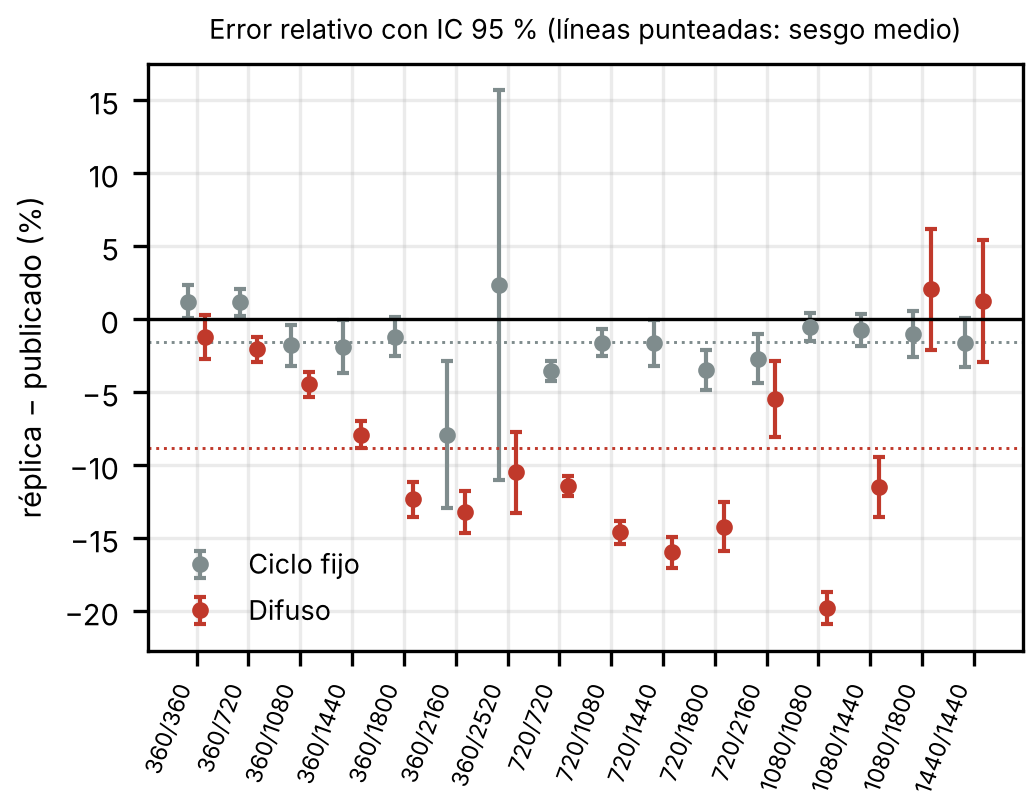
\includegraphics[width=\columnwidth]{fig_incertidumbre.png}
\caption{Error relativo (réplica $-$ publicado) con IC 95\,\% en cada caudal, para el ciclo fijo y el controlador difuso. Las líneas punteadas son el sesgo medio de cada serie.}
\label{fig:incertidumbre}
\end{figure}

\begin{table}[!t]
\caption{Incertidumbre estadística de la réplica (20 réplicas de 7200\,s, lectura calibrada): retardo medio $\pm$ semiancho del IC al 95\,\%, valor publicado y marca ($\checkmark$) si el valor publicado cae dentro del intervalo. Mejora en \% sobre el ciclo fijo simulado; en las 16 combinaciones $p<0.001$ (Welch).}
\label{tab:estadistica}
\centering
\scriptsize
\setlength{\tabcolsep}{2.2pt}
\begin{tabular}{@{}lrrcrrcr@{}}
\toprule
 & \multicolumn{3}{c}{Ciclo fijo (s)} & \multicolumn{3}{c}{Difuso (s)} & \\
\cmidrule(lr){2-4}\cmidrule(lr){5-7}
N-S/E-W & Réplica & Pub. & En IC & Réplica & Pub. & En IC & Mej. \\
\midrule
360/360 & 7.29\,$\pm$\,0.08 & 7.2 &  & 5.63\,$\pm$\,0.09 & 5.7 & \checkmark & 22.7 \\
360/720 & 7.48\,$\pm$\,0.07 & 7.4 &  & 5.97\,$\pm$\,0.05 & 6.1 &  & 20.2 \\
360/1080 & 7.76\,$\pm$\,0.11 & 7.9 &  & 6.30\,$\pm$\,0.06 & 6.6 &  & 18.7 \\
360/1440 & 8.24\,$\pm$\,0.15 & 8.4 &  & 6.72\,$\pm$\,0.07 & 7.3 &  & 18.4 \\
360/1800 & 9.19\,$\pm$\,0.12 & 9.3 & \checkmark & 7.36\,$\pm$\,0.10 & 8.4 &  & 19.9 \\
360/2160 & 11.33\,$\pm$\,0.62 & 12.3 &  & 8.68\,$\pm$\,0.14 & 10.0 &  & 23.4 \\
360/2520 & 16.17\,$\pm$\,2.11 & 15.8 & \checkmark & 12.17\,$\pm$\,0.38 & 13.6 &  & 24.7 \\
720/720 & 9.36\,$\pm$\,0.07 & 9.7 &  & 6.55\,$\pm$\,0.05 & 7.4 &  & 30.0 \\
720/1080 & 10.63\,$\pm$\,0.10 & 10.8 &  & 7.52\,$\pm$\,0.07 & 8.8 &  & 29.3 \\
720/1440 & 12.49\,$\pm$\,0.20 & 12.7 &  & 9.16\,$\pm$\,0.12 & 10.9 &  & 26.7 \\
720/1800 & 15.35\,$\pm$\,0.22 & 15.9 &  & 12.10\,$\pm$\,0.24 & 14.1 &  & 21.2 \\
720/2160 & 21.21\,$\pm$\,0.36 & 21.8 &  & 17.49\,$\pm$\,0.48 & 18.5 &  & 17.6 \\
1080/1080 & 13.53\,$\pm$\,0.13 & 13.6 & \checkmark & 9.62\,$\pm$\,0.13 & 12.0 &  & 28.8 \\
1080/1440 & 17.77\,$\pm$\,0.20 & 17.9 & \checkmark & 13.63\,$\pm$\,0.32 & 15.4 &  & 23.3 \\
1080/1800 & 25.54\,$\pm$\,0.41 & 25.8 & \checkmark & 22.04\,$\pm$\,0.90 & 21.6 & \checkmark & 13.7 \\
1440/1440 & 26.86\,$\pm$\,0.47 & 27.3 & \checkmark & 23.18\,$\pm$\,0.96 & 22.9 & \checkmark & 13.7 \\
\midrule
\multicolumn{3}{@{}l}{Publicado dentro del IC} & 6/16 & & & 3/16 & \\
\multicolumn{3}{@{}l}{Sesgo medio réplica$-$publicado (\%)} & -1.6 & & & -8.8 & \\
\bottomrule
\end{tabular}
\fuente{\texttt{analisis\_estadistico.py} (\texttt{resultados/analisis\_estadistico.json}), con las 20 réplicas de cada celda; valores «Pub.»: Tabla~I (ciclo fijo, p.~708) y Tabla~VIII (difuso, p.~715) del artículo original. IC con la distribución $t$ de Student ($n=20$); mejora contrastada con la prueba de Welch.}
\end{table}


\subsection{Auditoría de las lecturas}
\label{sec:auditoria}
La Tabla~\ref{tab:auditoria} y la Fig.~\ref{fig:auditoria} muestran el resultado de las ocho lecturas. Solo una, la calibrada, reproduce la Tabla~VIII en todo el rango (error medio 9.3\,\%, máximo 19.3\,\% con 10 réplicas); las otras siete tienen un error medio superior a 175\,\% y empeoran sobre todo con caudales altos. La razón es estructural: con la cola total real del brazo en rojo, las reglas de 7, 17 y 27\,s solo extienden si esa cola es de unos 5 vehículos o menos (\emph{lt}(very small)); en cuanto el flujo sube se corta el verde hacia los 9\,s, la capacidad no alcanza y el sistema se satura. La lectura calibrada es sensible: contar la cola completa, o los dos vehículos que llegan durante el tiempo perdido, la vuelve inestable.

\begin{table}[!t]
\caption{Auditoría de las ocho lecturas de las entradas del controlador (reglas fijas; 10 réplicas de 7200\,s). Error relativo frente a la Tabla VIII del artículo.}
\label{tab:auditoria}
\centering
\scriptsize
\setlength{\tabcolsep}{2.4pt}
\begin{tabular}{@{}lllrrr@{}}
\toprule
$A$ & $Q$ evaluada & Cola $Q$ & Medio\,\% & Máx.\,\% & Mejor que fijo \\
\midrule
arribos & predicha & total & 631.0 & 2623 & 5/16 (literal) \\
arribos & predicha & desde el verde & 323.1 & 1869 & 6/16 \\
arribos & actual & total & 566.6 & 2610 & 5/16 \\
arribos & actual & desde el verde & 227.6 & 1185 & 6/16 \\
cruces & predicha & total & 421.0 & 2404 & 11/16 \\
cruces & predicha & desde el verde & 175.4 & 1162 & 11/16 \\
cruces & actual & total & 374.1 & 2362 & 12/16 \\
cruces & actual & desde el verde & 9.3 & 19 & 16/16 (calibrada) \\
\bottomrule
\end{tabular}
\fuente{simulaciones propias (\texttt{fidelity\_audit.py}, \texttt{resultados/fidelity\_audit.json}) comparadas con la Tabla~VIII del artículo original (p.~715).}
\end{table}


\begin{figure}[!t]
\centering
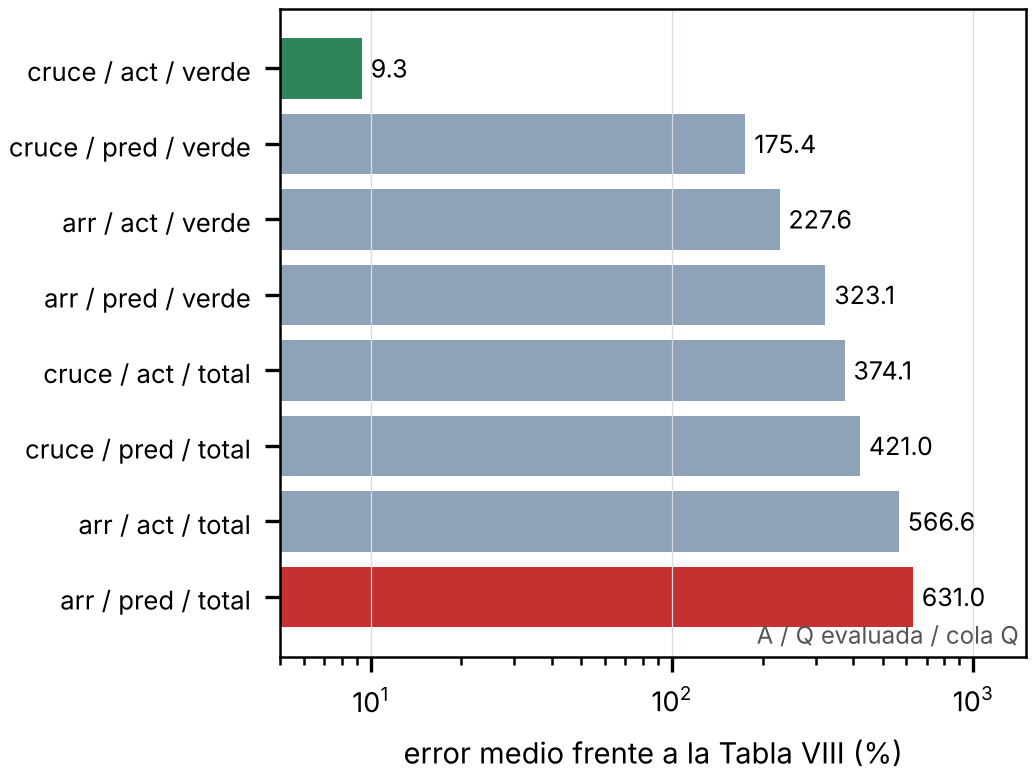
\includegraphics[width=\columnwidth]{fig_auditoria.png}
\caption{Error medio de cada lectura de $A$ y $Q$ frente a la Tabla~VIII (escala logarítmica). En verde la lectura calibrada y en rojo la literal.}
\label{fig:auditoria}
\end{figure}

\subsection{Llegadas aleatorias frente a llegadas fijas}
El artículo describe llegadas aleatorias en cada segundo; una entrada fija de 1\,veh/s por brazo equivaldría a 3600\,veh/h, mientras que sus tablas usan entre 360 y 2520\,veh/h. Se comprobó además la alternativa de llegadas fijas (Tabla~\ref{tab:llegadas}): con ellas el ciclo fijo queda sistemáticamente por debajo de la Tabla~I (error medio de 10.4\,\% frente a 2.0\,\% con llegadas aleatorias). La Tabla~VIII no distingue entre ambos modelos. La Tabla~I respalda, por tanto, las llegadas aleatorias.

\begin{table}[!t]
\caption{Llegadas aleatorias frente a llegadas fijas (un vehículo cada $1/\lambda$ segundos): error relativo medio respecto del artículo (10 réplicas de 7200\,s).}
\label{tab:llegadas}
\centering
\footnotesize
\begin{tabular}{@{}lcc@{}}
\toprule
Modelo de llegadas & Tabla I (\%) & Tabla VIII (\%) \\
\midrule
Aleatorias (Bernoulli por segundo) & 2.0 & 9.3 \\
Fijas & 10.4 & 10.0 \\
\bottomrule
\end{tabular}
\fuente{simulaciones propias (\texttt{arrival\_model\_check.py}, \texttt{resultados/llegadas\_fijas\_vs\_aleatorias.json}) comparadas con las Tablas~I y~VIII del artículo original (pp.~708 y~715).}
\end{table}


\subsection{Reglas usadas y disparos en la simulación}
\label{sec:reglas-disparos}
La Fig.~\ref{fig:disparos} muestra qué reglas deciden en una simulación de 1800\,s con 720/2160\,veh/h y lectura calibrada. De las 148 decisiones, 11 fueron cortes del verde y 137 extensiones; en 114 de estas últimas la regla que dispara es la de extensión muy larga (R5 de cada intervención), y la extensión elegida es de 10\,s. Las reglas intermedias se activan con frecuencia pero casi nunca deciden.

\begin{figure*}[!t]
\centering
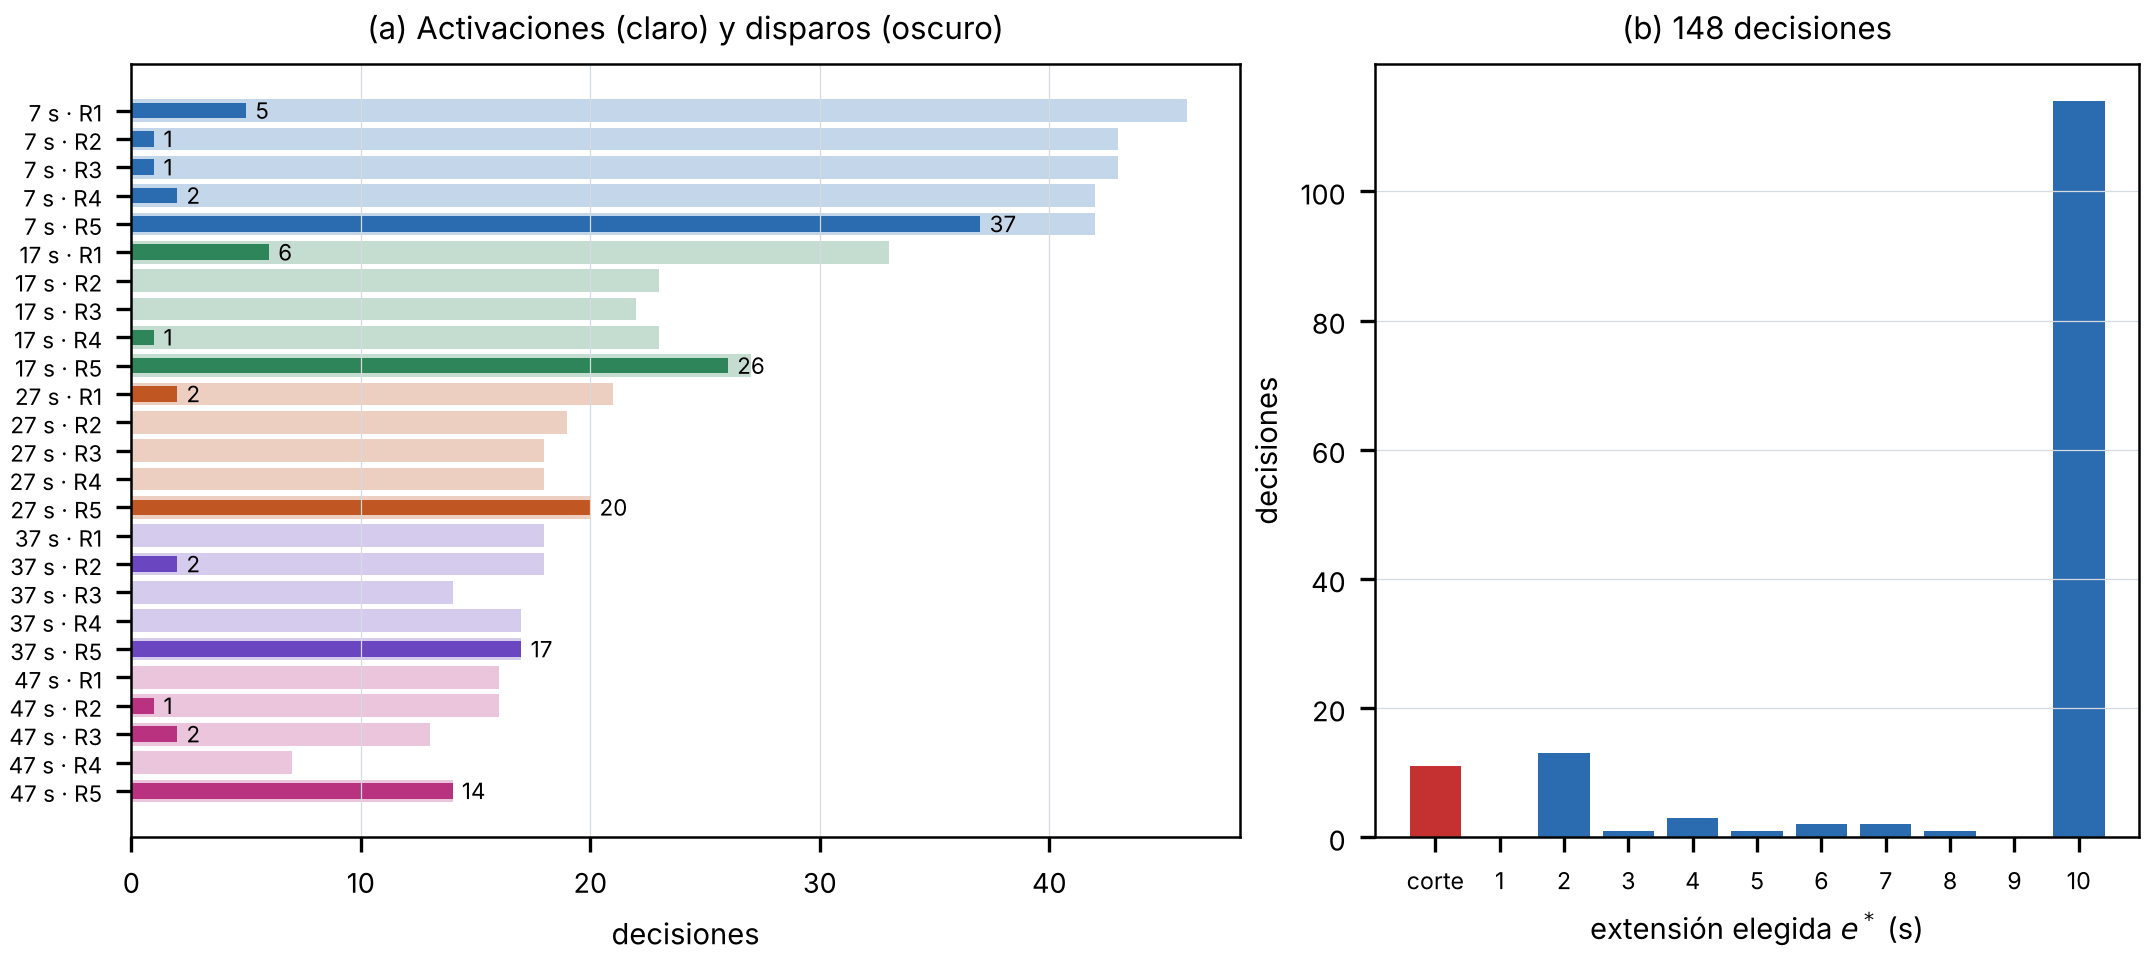
\includegraphics[width=0.92\textwidth]{fig_disparos.png}
\caption{Reglas usadas en una simulación (720/2160\,veh/h, 1800\,s, lectura calibrada): (a) activaciones y disparos de cada una de las 25 reglas; (b) distribución de la extensión elegida.}
\label{fig:disparos}
\end{figure*}

Para estimar cuántas reglas son necesarias se realizó un experimento exploratorio que conserva las reglas del artículo y quita algunas (Tabla~\ref{tab:ablacion}). Conservar solo las reglas extremas (10 reglas) o tres por intervención (15) da el mismo retardo medio que las 25, dentro del ruido de 10 réplicas; usar una sola base para todas las intervenciones lo empeora claramente, lo que muestra que importa que haya una base por intervención; y conservar solo la regla de extensión más corta colapsa el sistema. El experimento se hizo con una única lectura de las entradas y pocas réplicas, por lo que no demuestra que 10 reglas sean mejores en general.

\begin{table}[!t]
\caption{Reducción de reglas (lectura calibrada; 20 réplicas de 7200\,s con números aleatorios comunes). $d_m$: retardo medio de los 16 flujos por réplica (media $\pm$ desviación estándar). «Dif.»: respecto de las 25 reglas; $p$: Wilcoxon pareado con Holm. «Mej. fijo»: flujos en que mejora al ciclo fijo. Friedman entre las 6 variantes: $\chi^2_5=93.5$, $p<0.001$.}
\label{tab:ablacion}
\centering
\scriptsize
\setlength{\tabcolsep}{1.6pt}
\begin{tabular}{@{}cp{0.27\columnwidth}rrrrr@{}}
\toprule
 & Reglas conservadas & N.º & $d_m$ (s) & Dif.\,\% & $p$ & Mej. fijo \\
\midrule
A & Original: 5 reglas por intervención & 25 & 10.93\,$\pm$\,0.42 & --- & --- & 16/16 \\
B & Una sola base (la de 7 s) en las 5 intervenciones & 5 & 16.97\,$\pm$\,3.27 & +55.3 & $<0.001$ & 13/16 \\
C & Sin la regla veryshort & 20 & 11.45\,$\pm$\,0.52 & +4.8 & $<0.001$ & 16/16 \\
D & Tres reglas (veryshort, medium, verylong) & 15 & 11.10\,$\pm$\,0.41 & +1.6 & $<0.001$ & 16/16 \\
E & Solo extremos (veryshort, verylong) & 10 & 11.38\,$\pm$\,0.41 & +4.1 & $<0.001$ & 16/16 \\
F & Solo veryshort & 5 & 351.76\,$\pm$\,10.08 & +3118.3 & $<0.001$ & 3/16 \\
\bottomrule
\end{tabular}
\fuente{simulaciones propias (\texttt{ablacion\_reglas.py}) con subconjuntos de las reglas del Apéndice del artículo original (pp.~715 y~716); línea base: ciclo fijo de la Tabla~I.}
\end{table}


\subsection{Desglose por intervención}
La Tabla~\ref{tab:intervenciones} separa las decisiones según el instante de intervención. Las decisiones disminuyen de 49 en la intervención de 7\,s a 17 en la de 47\,s, porque un verde solo llega a una intervención tardía si las anteriores lo extendieron. En todas las intervenciones, la extensión máxima de 10\,s coincide con el disparo de la regla R5: 114 de 114 casos. Los cortes del verde ($e^*=0$) son 11 y aparecen sobre todo en las primeras intervenciones; la tabla no permite atribuirlos a una causa concreta.

La activación media de las reglas intermedias (R2--R4) es comparable a la de R5 en la intervención de 7\,s (entre 0.65 y 0.76), pero estas reglas casi no deciden porque el grado de la extensión de 10\,s es mayor en la mayoría de los casos. Esto es coherente con el diseño del artículo: las cinco reglas de cada intervención solapan sus conclusiones y la decisión se toma por el máximo de grado, de modo que una regla activa no implica una regla que dispara. En la intervención de 47\,s la regla R4 se activa en solo 7 de 17 decisiones, lo que indica que la combinación de antecedentes que la define es rara en este régimen de tráfico.

\begin{table}[!t]
\caption{Decisiones por intervención en la simulación de la Fig.~\ref{fig:disparos} (cortes: $e^*{=}0$)}
\label{tab:intervenciones}
\centering
\footnotesize
\begin{tabular}{rrrrr}
\hline
Interv. (s) & Decis. & Cortes & $e^*{=}10$ & R5 dispara \\
\hline
7  & 49 & 3 & 37 & 37 \\
17  & 36 & 3 & 26 & 26 \\
27  & 26 & 4 & 20 & 20 \\
37  & 20 & 1 & 17 & 17 \\
47  & 17 & 0 & 14 & 14 \\
\hline
Total & 148 & 11 & 114 & 114 \\
\hline
\end{tabular}
\fuente{conteo propio sobre \texttt{muestras/disparos\_reglas.csv} (\texttt{informe\_disparos.py}: 720/2160\,veh/h, 1800\,s, semilla 1, lectura calibrada). Una decisión es una intervención del controlador; $e^*$ se obtiene con \eqref{eq:decision}.}
\end{table}


\subsection{Amenazas a la validez}
\textit{Validez interna.} Las cifras de esta sección provienen de una sola semilla y de 1800\,s simulados, por lo que describen un régimen y no una distribución; sirven para mostrar el mecanismo de disparo y no para estimar frecuencias poblacionales. \textit{Validez de construcción.} La lectura calibrada de $A$ y $Q$ es una inferencia por falta de datos; con la lectura literal las frecuencias de disparo serían distintas. \textit{Validez externa.} Los resultados corresponden a una intersección aislada de dos fases con saturación de 1\,veh/s, igual que el artículo original, y no deben extrapolarse a redes ni a flujos con giros.

% =============================================================================
\section{Discusión}
\label{sec:discusion}

\subsection{Qué se reproduce y qué se infiere}
Todo lo que el artículo especifica se reproduce exactamente o dentro de la variabilidad estadística: conjuntos, operadores, reglas, ejemplo, tiempos, modelo y Tabla~I. La conclusión cualitativa de la Tabla~VIII (el difuso supera al ciclo fijo en todas las combinaciones, con mejoras de un orden comparable) también se reproduce, pero solo con una lectura de las entradas que no está en el texto. Esa lectura es, por tanto, una inferencia por falta de datos, y los resultados de la Tabla~VIII deben leerse con esa salvedad.

\subsection{Información ausente en el artículo}
La Tabla~\ref{tab:ausente} reúne los datos que el artículo no contiene y la decisión adoptada en la réplica.

\begin{table*}[!t]
\caption{Información que el artículo original no contiene y decisión adoptada en la réplica}
\label{tab:ausente}
\centering
\footnotesize
\setlength{\tabcolsep}{3pt}
\begin{tabular}{@{}p{0.22\textwidth}p{0.36\textwidth}p{0.36\textwidth}@{}}
\toprule
Dato ausente & Qué dice el artículo & Decisión en la réplica \\
\midrule
Cálculo de $A$ y $Q$ en cada intervención & El ejemplo da vectores ya calculados ($\beta$ y $\beta'$) & Dos lecturas; la calibrada se infiere por reproducir la Tabla~VIII (inferencia) \\
Velocidades y distancia de los detectores & Cada vehículo se registra con $N=l/v-1.5$\,s sin dar $l$ ni $v$ & No se modela; los arribos por segundo son los cruces del punto crítico (suposición) \\
Valores fuera de los universos & Colas de 4 a 32 y arribos de 1 a 10 & $\mu_{lt}(q)=1$ para $q<4$; $\mu_{mt}(0)=0$ (suposición) \\
Réplicas, semillas y generador aleatorio & «Muchas corridas»; 7200\,s; computador ICL-1900 & 20 réplicas de 7200\,s, semilla base 0 \\
Condiciones iniciales & No se mencionan & Colas vacías, empieza la fase N--S, sin calentamiento \\
Reparto del tiempo perdido & 10\,s por ciclo; ámbar de 3\,s con verde efectivo hasta su mitad & 5\,s sin descarga por cambio de fase; sus arribos se acumulan \\
\bottomrule
\end{tabular}
\fuente{revisión propia del texto del artículo original (pp.~707 a~717); la columna central cita lo que el artículo dice y la derecha, la decisión tomada en este trabajo.}
\end{table*}

\subsection{Tamaño de la base de reglas}
Al combinar todas las etiquetas de las tres entradas se obtienen $5\times6\times6=180$ combinaciones de antecedentes por intervención (900 para las cinco; es el producto del número de etiquetas de las Tablas~II a~IV, p.~711), que se listan completas en el Apéndice~\ref{app:180}. Las 25 reglas del artículo ocupan solo 19 de esas 180 combinaciones; las otras 161 no tienen regla propia. El artículo utiliza 25 reglas, por varias razones: cada regla establece qué se exige para una etiqueta de salida; los operadores \emph{mt} y \emph{lt} hacen que una regla cubra una región completa del espacio de entradas («al menos \emph{many}», «menos que \emph{small}»), de modo que la rejilla completa sería muy redundante; el tiempo no entra como una cuarta variable sino como una base de reglas por intervención; y las reglas proceden de un protocolo de operador humano afinado por prueba y error. Ese diseño evita el crecimiento exponencial de una base completa, un problema general del control difuso.

La literatura revisada ofrece alternativas con menos reglas o con ajuste automático: los consecuentes funcionales de Takagi y Sugeno \cite{TakagiSugeno1985}, la descomposición en etapas o subsistemas de Trabia \emph{et al.} \cite{Trabia1999} y de Murat y Gedizlioglu \cite{Murat2005}, el ajuste de funciones de pertenencia por aprendizaje \cite{Jang1993,Bingham2001} y el aprendizaje por refuerzo \cite{Abdulhai2003}. Si un modelo es «más eficiente» depende del criterio (número de reglas, retardo o esfuerzo de ajuste), y en las fuentes revisadas no se encontró una comparación directa de número de reglas frente a retardo para este controlador. El experimento de la Sección~\ref{sec:reglas-disparos} sugiere que, en la réplica, pocas reglas extremas concentran la decisión.

\subsection{Reproducibilidad de este trabajo}
Siguiendo la idea de las listas de verificación de reproducibilidad \cite{Pineau2021,Sandve2013}, la Tabla~\ref{tab:repro} indica qué se publica aquí para que otras personas repitan o auditen los resultados.

\begin{table}[!t]
\caption{Elementos de reproducibilidad de este trabajo}
\label{tab:repro}
\centering
\footnotesize
\setlength{\tabcolsep}{3pt}
\begin{tabular}{@{}p{0.3\columnwidth}p{0.6\columnwidth}@{}}
\toprule
Elemento & Qué se publica \\
\midrule
Código & Modelo, controlador, motor paso a paso y simulador gráfico \\
Valores de referencia & Valores impresos del artículo transcritos de las imágenes y pruebas que los comparan con el código \\
Protocolo & 20 réplicas de 7200\,s, semilla base 0, 16 caudales \\
Resultados & Archivos con todas las cifras de las tablas y la auditoría \\
Decisiones & Lecturas de las entradas y supuestos, declarados como tales \\
Figuras y tablas & Generadas por programa a partir de esos archivos \\
\bottomrule
\end{tabular}
\fuente{elaboración propia: archivos del proyecto que acompaña a este manuscrito (carpetas \texttt{codigo/}, \texttt{resultados/} y \texttt{articulo\_ieee/}).}
\end{table}

\subsection{Limitaciones}
La réplica es estadística y no dígito a dígito: no se dispone del programa ni del generador aleatorio de 1977. El difuso simulado queda en promedio $8.8$\,\% por debajo de lo publicado (hasta 19.8\,\% en una celda), un sesgo estadísticamente significativo (Sección~\ref{sec:estadistica}) que no se corrigió con ajustes de las reglas, porque eso modificaría el método replicado. El experimento de reducción de reglas y la comparación de llegadas se hicieron con pocas réplicas y una sola lectura. Por último, la revisión de la literatura se limita a las fuentes citadas.

% =============================================================================
\section{Conclusiones}
\label{sec:conclusiones}

Se replicó el controlador de lógica difusa de Pappis y Mamdani a partir de la publicación original y se validó elemento por elemento: los conjuntos y operadores coinciden exactamente con las tablas impresas, las 25 reglas se transcribieron de la imagen del original corrigiendo errores de transcripción, el ejemplo trabajado se reproduce en cada fila, y la tabla de validación del modelo se reproduce con un error medio de 2.1\,\%. La tabla de resultados del controlador se reproduce en su conclusión cualitativa (mejora al ciclo fijo en 16 de 16 combinaciones, con $p<0.001$ en todas; error medio de 9.3\,\%), aunque con un sesgo sistemático de $-8.8$\,\% en el retardo del difuso respecto de lo publicado, pero solo con una lectura de las entradas que el artículo no especifica; de ocho lecturas plausibles, solo una lo logra, y se presenta como inferencia por falta de datos.

Como aportes adicionales, la comparación de llegadas respalda el modelo aleatorio, un simulador abierto muestra las reglas usadas y los disparos de cada decisión, y un experimento exploratorio indica que unas pocas reglas extremas concentran la decisión en la réplica. Como trabajo futuro se propone repetir el experimento de reducción de reglas con más réplicas y con otras lecturas de las entradas, comparar el controlador con variantes de Takagi y Sugeno y con aprendizaje por refuerzo bajo el mismo protocolo, y aplicar el protocolo de réplica a otros controladores difusos de semáforos.

% =============================================================================
\clearpage
\onecolumn
\appendices
\section{Las 180 reglas del espacio $T\times A\times Q$}
\label{app:180}
Las tablas siguientes escriben literalmente las $5\times6\times6=180$ reglas que resultan de combinar las etiquetas de tiempo $T$ (very short, short, medium, long, very long), de arribos $A$ (none, a few, few, medium, many, too many) y de cola $Q$ (very small, small, small plus, medium, long, very long), con $E=T$ en todas. El artículo original emplea 25 de ellas: cinco reglas (R1 a R5) en cada una de las cinco intervenciones. Las reglas del autor aparecen resaltadas en verde y con $\checkmark$; las 161 restantes, con $\times$. Las cinco columnas de intervención indican, para cada regla, con qué número de regla la usa cada intervención. Los mismos datos están en \texttt{resultados/reglas\_180.csv}.

La cuenta de las 25 reglas se lee en las columnas de intervención. Las reglas R2 a R5 de cada intervención son una regla cada una (20 en total). La regla R1 de cada intervención (5 en total) no condiciona la cola, por lo que en el listado de 180 reglas ocupa las seis filas de $T=$ very short y $A=$ none (marcada R1*). Como varias reglas coinciden entre intervenciones, las 25 reglas del autor ocupan solo 19 filas de las 180.

{\scriptsize
\setlength{\tabcolsep}{3pt}
\renewcommand{\arraystretch}{1.0}
\begin{longtable}{@{}r l ccccc c@{}}
\caption{Las 180 reglas del espacio $T\times A\times Q$ ($5\times6\times6$; cada una concluye $E=T$). Las que usa el autor están resaltadas en verde y marcadas con $\checkmark$; las demás, con $\times$. Las columnas de intervención indican con qué número de regla (R1 a R5) la usa cada intervención; R1* es la regla R1 del autor, que usa $Q=$ any (no condiciona la cola) y por eso cubre las seis reglas de su fila.}
\label{tab:180}\\
\toprule
\# & Regla & 7\,s & 17\,s & 27\,s & 37\,s & 47\,s & Usada \\
\midrule
\endfirsthead
\toprule
\# & Regla & 7\,s & 17\,s & 27\,s & 37\,s & 47\,s & Usada \\
\midrule
\endhead
\midrule
\multicolumn{8}{r}{\textit{continúa en la página siguiente}}\\
\endfoot
\bottomrule
\multicolumn{8}{@{}p{0.98\textwidth}@{}}{\vspace{2pt}\textit{Fuente:} etiquetas de $T$, $A$ y $Q$ de las Tablas~II a~IV del artículo original (p.~711), combinadas por la regla del producto ($5\times6\times6=180$); reglas resaltadas: Apéndice del artículo original (pp.~715 y~716). Código: \texttt{gen\_tabla\_180.py}; mismos datos en \texttt{resultados/reglas\_180.csv}.}\\
\endlastfoot
\rowcolor{green!14}1 & \textbf{SI} $T$ = very short \textbf{Y} $A$ = mt(none) \textbf{Y} $Q$ = lt(very small) \textbf{ENTONCES} $E$ = very short & \cellcolor{green!35}R1* & \cellcolor{green!35}R1* & \cellcolor{green!35}R1* & \cellcolor{green!35}R1* & \cellcolor{green!35}R1* & \textbf{\checkmark} \\
\rowcolor{green!14}2 & \textbf{SI} $T$ = very short \textbf{Y} $A$ = mt(none) \textbf{Y} $Q$ = lt(small) \textbf{ENTONCES} $E$ = very short & \cellcolor{green!35}R1* & \cellcolor{green!35}R1* & \cellcolor{green!35}R1* & \cellcolor{green!35}R1* & \cellcolor{green!35}R1* & \textbf{\checkmark} \\
\rowcolor{green!14}3 & \textbf{SI} $T$ = very short \textbf{Y} $A$ = mt(none) \textbf{Y} $Q$ = lt(small plus) \textbf{ENTONCES} $E$ = very short & \cellcolor{green!35}R1* & \cellcolor{green!35}R1* & \cellcolor{green!35}R1* & \cellcolor{green!35}R1* & \cellcolor{green!35}R1* & \textbf{\checkmark} \\
\rowcolor{green!14}4 & \textbf{SI} $T$ = very short \textbf{Y} $A$ = mt(none) \textbf{Y} $Q$ = lt(medium) \textbf{ENTONCES} $E$ = very short & \cellcolor{green!35}R1* & \cellcolor{green!35}R1* & \cellcolor{green!35}R1* & \cellcolor{green!35}R1* & \cellcolor{green!35}R1* & \textbf{\checkmark} \\
\rowcolor{green!14}5 & \textbf{SI} $T$ = very short \textbf{Y} $A$ = mt(none) \textbf{Y} $Q$ = lt(long) \textbf{ENTONCES} $E$ = very short & \cellcolor{green!35}R1* & \cellcolor{green!35}R1* & \cellcolor{green!35}R1* & \cellcolor{green!35}R1* & \cellcolor{green!35}R1* & \textbf{\checkmark} \\
\rowcolor{green!14}6 & \textbf{SI} $T$ = very short \textbf{Y} $A$ = mt(none) \textbf{Y} $Q$ = lt(very long) \textbf{ENTONCES} $E$ = very short & \cellcolor{green!35}R1* & \cellcolor{green!35}R1* & \cellcolor{green!35}R1* & \cellcolor{green!35}R1* & \cellcolor{green!35}R1* & \textbf{\checkmark} \\
7 & \textbf{SI} $T$ = very short \textbf{Y} $A$ = mt(a few) \textbf{Y} $Q$ = lt(very small) \textbf{ENTONCES} $E$ = very short &  &  &  &  &  & $\times$ \\
8 & \textbf{SI} $T$ = very short \textbf{Y} $A$ = mt(a few) \textbf{Y} $Q$ = lt(small) \textbf{ENTONCES} $E$ = very short &  &  &  &  &  & $\times$ \\
9 & \textbf{SI} $T$ = very short \textbf{Y} $A$ = mt(a few) \textbf{Y} $Q$ = lt(small plus) \textbf{ENTONCES} $E$ = very short &  &  &  &  &  & $\times$ \\
10 & \textbf{SI} $T$ = very short \textbf{Y} $A$ = mt(a few) \textbf{Y} $Q$ = lt(medium) \textbf{ENTONCES} $E$ = very short &  &  &  &  &  & $\times$ \\
11 & \textbf{SI} $T$ = very short \textbf{Y} $A$ = mt(a few) \textbf{Y} $Q$ = lt(long) \textbf{ENTONCES} $E$ = very short &  &  &  &  &  & $\times$ \\
12 & \textbf{SI} $T$ = very short \textbf{Y} $A$ = mt(a few) \textbf{Y} $Q$ = lt(very long) \textbf{ENTONCES} $E$ = very short &  &  &  &  &  & $\times$ \\
13 & \textbf{SI} $T$ = very short \textbf{Y} $A$ = mt(few) \textbf{Y} $Q$ = lt(very small) \textbf{ENTONCES} $E$ = very short &  &  &  &  &  & $\times$ \\
14 & \textbf{SI} $T$ = very short \textbf{Y} $A$ = mt(few) \textbf{Y} $Q$ = lt(small) \textbf{ENTONCES} $E$ = very short &  &  &  &  &  & $\times$ \\
15 & \textbf{SI} $T$ = very short \textbf{Y} $A$ = mt(few) \textbf{Y} $Q$ = lt(small plus) \textbf{ENTONCES} $E$ = very short &  &  &  &  &  & $\times$ \\
16 & \textbf{SI} $T$ = very short \textbf{Y} $A$ = mt(few) \textbf{Y} $Q$ = lt(medium) \textbf{ENTONCES} $E$ = very short &  &  &  &  &  & $\times$ \\
17 & \textbf{SI} $T$ = very short \textbf{Y} $A$ = mt(few) \textbf{Y} $Q$ = lt(long) \textbf{ENTONCES} $E$ = very short &  &  &  &  &  & $\times$ \\
18 & \textbf{SI} $T$ = very short \textbf{Y} $A$ = mt(few) \textbf{Y} $Q$ = lt(very long) \textbf{ENTONCES} $E$ = very short &  &  &  &  &  & $\times$ \\
19 & \textbf{SI} $T$ = very short \textbf{Y} $A$ = mt(medium) \textbf{Y} $Q$ = lt(very small) \textbf{ENTONCES} $E$ = very short &  &  &  &  &  & $\times$ \\
20 & \textbf{SI} $T$ = very short \textbf{Y} $A$ = mt(medium) \textbf{Y} $Q$ = lt(small) \textbf{ENTONCES} $E$ = very short &  &  &  &  &  & $\times$ \\
21 & \textbf{SI} $T$ = very short \textbf{Y} $A$ = mt(medium) \textbf{Y} $Q$ = lt(small plus) \textbf{ENTONCES} $E$ = very short &  &  &  &  &  & $\times$ \\
22 & \textbf{SI} $T$ = very short \textbf{Y} $A$ = mt(medium) \textbf{Y} $Q$ = lt(medium) \textbf{ENTONCES} $E$ = very short &  &  &  &  &  & $\times$ \\
23 & \textbf{SI} $T$ = very short \textbf{Y} $A$ = mt(medium) \textbf{Y} $Q$ = lt(long) \textbf{ENTONCES} $E$ = very short &  &  &  &  &  & $\times$ \\
24 & \textbf{SI} $T$ = very short \textbf{Y} $A$ = mt(medium) \textbf{Y} $Q$ = lt(very long) \textbf{ENTONCES} $E$ = very short &  &  &  &  &  & $\times$ \\
25 & \textbf{SI} $T$ = very short \textbf{Y} $A$ = mt(many) \textbf{Y} $Q$ = lt(very small) \textbf{ENTONCES} $E$ = very short &  &  &  &  &  & $\times$ \\
26 & \textbf{SI} $T$ = very short \textbf{Y} $A$ = mt(many) \textbf{Y} $Q$ = lt(small) \textbf{ENTONCES} $E$ = very short &  &  &  &  &  & $\times$ \\
27 & \textbf{SI} $T$ = very short \textbf{Y} $A$ = mt(many) \textbf{Y} $Q$ = lt(small plus) \textbf{ENTONCES} $E$ = very short &  &  &  &  &  & $\times$ \\
28 & \textbf{SI} $T$ = very short \textbf{Y} $A$ = mt(many) \textbf{Y} $Q$ = lt(medium) \textbf{ENTONCES} $E$ = very short &  &  &  &  &  & $\times$ \\
29 & \textbf{SI} $T$ = very short \textbf{Y} $A$ = mt(many) \textbf{Y} $Q$ = lt(long) \textbf{ENTONCES} $E$ = very short &  &  &  &  &  & $\times$ \\
30 & \textbf{SI} $T$ = very short \textbf{Y} $A$ = mt(many) \textbf{Y} $Q$ = lt(very long) \textbf{ENTONCES} $E$ = very short &  &  &  &  &  & $\times$ \\
31 & \textbf{SI} $T$ = very short \textbf{Y} $A$ = mt(too many) \textbf{Y} $Q$ = lt(very small) \textbf{ENTONCES} $E$ = very short &  &  &  &  &  & $\times$ \\
32 & \textbf{SI} $T$ = very short \textbf{Y} $A$ = mt(too many) \textbf{Y} $Q$ = lt(small) \textbf{ENTONCES} $E$ = very short &  &  &  &  &  & $\times$ \\
33 & \textbf{SI} $T$ = very short \textbf{Y} $A$ = mt(too many) \textbf{Y} $Q$ = lt(small plus) \textbf{ENTONCES} $E$ = very short &  &  &  &  &  & $\times$ \\
34 & \textbf{SI} $T$ = very short \textbf{Y} $A$ = mt(too many) \textbf{Y} $Q$ = lt(medium) \textbf{ENTONCES} $E$ = very short &  &  &  &  &  & $\times$ \\
35 & \textbf{SI} $T$ = very short \textbf{Y} $A$ = mt(too many) \textbf{Y} $Q$ = lt(long) \textbf{ENTONCES} $E$ = very short &  &  &  &  &  & $\times$ \\
36 & \textbf{SI} $T$ = very short \textbf{Y} $A$ = mt(too many) \textbf{Y} $Q$ = lt(very long) \textbf{ENTONCES} $E$ = very short &  &  &  &  &  & $\times$ \\
\midrule
37 & \textbf{SI} $T$ = short \textbf{Y} $A$ = mt(none) \textbf{Y} $Q$ = lt(very small) \textbf{ENTONCES} $E$ = short &  &  &  &  &  & $\times$ \\
38 & \textbf{SI} $T$ = short \textbf{Y} $A$ = mt(none) \textbf{Y} $Q$ = lt(small) \textbf{ENTONCES} $E$ = short &  &  &  &  &  & $\times$ \\
39 & \textbf{SI} $T$ = short \textbf{Y} $A$ = mt(none) \textbf{Y} $Q$ = lt(small plus) \textbf{ENTONCES} $E$ = short &  &  &  &  &  & $\times$ \\
40 & \textbf{SI} $T$ = short \textbf{Y} $A$ = mt(none) \textbf{Y} $Q$ = lt(medium) \textbf{ENTONCES} $E$ = short &  &  &  &  &  & $\times$ \\
41 & \textbf{SI} $T$ = short \textbf{Y} $A$ = mt(none) \textbf{Y} $Q$ = lt(long) \textbf{ENTONCES} $E$ = short &  &  &  &  &  & $\times$ \\
42 & \textbf{SI} $T$ = short \textbf{Y} $A$ = mt(none) \textbf{Y} $Q$ = lt(very long) \textbf{ENTONCES} $E$ = short &  &  &  &  &  & $\times$ \\
\rowcolor{green!14}43 & \textbf{SI} $T$ = short \textbf{Y} $A$ = mt(a few) \textbf{Y} $Q$ = lt(very small) \textbf{ENTONCES} $E$ = short & \cellcolor{green!35}R2 & \cellcolor{green!35}R2 & \cellcolor{green!35}R2 &  &  & \textbf{\checkmark} \\
44 & \textbf{SI} $T$ = short \textbf{Y} $A$ = mt(a few) \textbf{Y} $Q$ = lt(small) \textbf{ENTONCES} $E$ = short &  &  &  &  &  & $\times$ \\
\rowcolor{green!14}45 & \textbf{SI} $T$ = short \textbf{Y} $A$ = mt(a few) \textbf{Y} $Q$ = lt(small plus) \textbf{ENTONCES} $E$ = short &  &  &  & \cellcolor{green!35}R2 &  & \textbf{\checkmark} \\
46 & \textbf{SI} $T$ = short \textbf{Y} $A$ = mt(a few) \textbf{Y} $Q$ = lt(medium) \textbf{ENTONCES} $E$ = short &  &  &  &  &  & $\times$ \\
\rowcolor{green!14}47 & \textbf{SI} $T$ = short \textbf{Y} $A$ = mt(a few) \textbf{Y} $Q$ = lt(long) \textbf{ENTONCES} $E$ = short &  &  &  &  & \cellcolor{green!35}R2 & \textbf{\checkmark} \\
48 & \textbf{SI} $T$ = short \textbf{Y} $A$ = mt(a few) \textbf{Y} $Q$ = lt(very long) \textbf{ENTONCES} $E$ = short &  &  &  &  &  & $\times$ \\
49 & \textbf{SI} $T$ = short \textbf{Y} $A$ = mt(few) \textbf{Y} $Q$ = lt(very small) \textbf{ENTONCES} $E$ = short &  &  &  &  &  & $\times$ \\
50 & \textbf{SI} $T$ = short \textbf{Y} $A$ = mt(few) \textbf{Y} $Q$ = lt(small) \textbf{ENTONCES} $E$ = short &  &  &  &  &  & $\times$ \\
51 & \textbf{SI} $T$ = short \textbf{Y} $A$ = mt(few) \textbf{Y} $Q$ = lt(small plus) \textbf{ENTONCES} $E$ = short &  &  &  &  &  & $\times$ \\
52 & \textbf{SI} $T$ = short \textbf{Y} $A$ = mt(few) \textbf{Y} $Q$ = lt(medium) \textbf{ENTONCES} $E$ = short &  &  &  &  &  & $\times$ \\
53 & \textbf{SI} $T$ = short \textbf{Y} $A$ = mt(few) \textbf{Y} $Q$ = lt(long) \textbf{ENTONCES} $E$ = short &  &  &  &  &  & $\times$ \\
54 & \textbf{SI} $T$ = short \textbf{Y} $A$ = mt(few) \textbf{Y} $Q$ = lt(very long) \textbf{ENTONCES} $E$ = short &  &  &  &  &  & $\times$ \\
55 & \textbf{SI} $T$ = short \textbf{Y} $A$ = mt(medium) \textbf{Y} $Q$ = lt(very small) \textbf{ENTONCES} $E$ = short &  &  &  &  &  & $\times$ \\
56 & \textbf{SI} $T$ = short \textbf{Y} $A$ = mt(medium) \textbf{Y} $Q$ = lt(small) \textbf{ENTONCES} $E$ = short &  &  &  &  &  & $\times$ \\
57 & \textbf{SI} $T$ = short \textbf{Y} $A$ = mt(medium) \textbf{Y} $Q$ = lt(small plus) \textbf{ENTONCES} $E$ = short &  &  &  &  &  & $\times$ \\
58 & \textbf{SI} $T$ = short \textbf{Y} $A$ = mt(medium) \textbf{Y} $Q$ = lt(medium) \textbf{ENTONCES} $E$ = short &  &  &  &  &  & $\times$ \\
59 & \textbf{SI} $T$ = short \textbf{Y} $A$ = mt(medium) \textbf{Y} $Q$ = lt(long) \textbf{ENTONCES} $E$ = short &  &  &  &  &  & $\times$ \\
60 & \textbf{SI} $T$ = short \textbf{Y} $A$ = mt(medium) \textbf{Y} $Q$ = lt(very long) \textbf{ENTONCES} $E$ = short &  &  &  &  &  & $\times$ \\
61 & \textbf{SI} $T$ = short \textbf{Y} $A$ = mt(many) \textbf{Y} $Q$ = lt(very small) \textbf{ENTONCES} $E$ = short &  &  &  &  &  & $\times$ \\
62 & \textbf{SI} $T$ = short \textbf{Y} $A$ = mt(many) \textbf{Y} $Q$ = lt(small) \textbf{ENTONCES} $E$ = short &  &  &  &  &  & $\times$ \\
63 & \textbf{SI} $T$ = short \textbf{Y} $A$ = mt(many) \textbf{Y} $Q$ = lt(small plus) \textbf{ENTONCES} $E$ = short &  &  &  &  &  & $\times$ \\
64 & \textbf{SI} $T$ = short \textbf{Y} $A$ = mt(many) \textbf{Y} $Q$ = lt(medium) \textbf{ENTONCES} $E$ = short &  &  &  &  &  & $\times$ \\
65 & \textbf{SI} $T$ = short \textbf{Y} $A$ = mt(many) \textbf{Y} $Q$ = lt(long) \textbf{ENTONCES} $E$ = short &  &  &  &  &  & $\times$ \\
66 & \textbf{SI} $T$ = short \textbf{Y} $A$ = mt(many) \textbf{Y} $Q$ = lt(very long) \textbf{ENTONCES} $E$ = short &  &  &  &  &  & $\times$ \\
67 & \textbf{SI} $T$ = short \textbf{Y} $A$ = mt(too many) \textbf{Y} $Q$ = lt(very small) \textbf{ENTONCES} $E$ = short &  &  &  &  &  & $\times$ \\
68 & \textbf{SI} $T$ = short \textbf{Y} $A$ = mt(too many) \textbf{Y} $Q$ = lt(small) \textbf{ENTONCES} $E$ = short &  &  &  &  &  & $\times$ \\
69 & \textbf{SI} $T$ = short \textbf{Y} $A$ = mt(too many) \textbf{Y} $Q$ = lt(small plus) \textbf{ENTONCES} $E$ = short &  &  &  &  &  & $\times$ \\
70 & \textbf{SI} $T$ = short \textbf{Y} $A$ = mt(too many) \textbf{Y} $Q$ = lt(medium) \textbf{ENTONCES} $E$ = short &  &  &  &  &  & $\times$ \\
71 & \textbf{SI} $T$ = short \textbf{Y} $A$ = mt(too many) \textbf{Y} $Q$ = lt(long) \textbf{ENTONCES} $E$ = short &  &  &  &  &  & $\times$ \\
72 & \textbf{SI} $T$ = short \textbf{Y} $A$ = mt(too many) \textbf{Y} $Q$ = lt(very long) \textbf{ENTONCES} $E$ = short &  &  &  &  &  & $\times$ \\
\midrule
73 & \textbf{SI} $T$ = medium \textbf{Y} $A$ = mt(none) \textbf{Y} $Q$ = lt(very small) \textbf{ENTONCES} $E$ = medium &  &  &  &  &  & $\times$ \\
74 & \textbf{SI} $T$ = medium \textbf{Y} $A$ = mt(none) \textbf{Y} $Q$ = lt(small) \textbf{ENTONCES} $E$ = medium &  &  &  &  &  & $\times$ \\
75 & \textbf{SI} $T$ = medium \textbf{Y} $A$ = mt(none) \textbf{Y} $Q$ = lt(small plus) \textbf{ENTONCES} $E$ = medium &  &  &  &  &  & $\times$ \\
76 & \textbf{SI} $T$ = medium \textbf{Y} $A$ = mt(none) \textbf{Y} $Q$ = lt(medium) \textbf{ENTONCES} $E$ = medium &  &  &  &  &  & $\times$ \\
77 & \textbf{SI} $T$ = medium \textbf{Y} $A$ = mt(none) \textbf{Y} $Q$ = lt(long) \textbf{ENTONCES} $E$ = medium &  &  &  &  &  & $\times$ \\
78 & \textbf{SI} $T$ = medium \textbf{Y} $A$ = mt(none) \textbf{Y} $Q$ = lt(very long) \textbf{ENTONCES} $E$ = medium &  &  &  &  &  & $\times$ \\
79 & \textbf{SI} $T$ = medium \textbf{Y} $A$ = mt(a few) \textbf{Y} $Q$ = lt(very small) \textbf{ENTONCES} $E$ = medium &  &  &  &  &  & $\times$ \\
80 & \textbf{SI} $T$ = medium \textbf{Y} $A$ = mt(a few) \textbf{Y} $Q$ = lt(small) \textbf{ENTONCES} $E$ = medium &  &  &  &  &  & $\times$ \\
81 & \textbf{SI} $T$ = medium \textbf{Y} $A$ = mt(a few) \textbf{Y} $Q$ = lt(small plus) \textbf{ENTONCES} $E$ = medium &  &  &  &  &  & $\times$ \\
82 & \textbf{SI} $T$ = medium \textbf{Y} $A$ = mt(a few) \textbf{Y} $Q$ = lt(medium) \textbf{ENTONCES} $E$ = medium &  &  &  &  &  & $\times$ \\
83 & \textbf{SI} $T$ = medium \textbf{Y} $A$ = mt(a few) \textbf{Y} $Q$ = lt(long) \textbf{ENTONCES} $E$ = medium &  &  &  &  &  & $\times$ \\
84 & \textbf{SI} $T$ = medium \textbf{Y} $A$ = mt(a few) \textbf{Y} $Q$ = lt(very long) \textbf{ENTONCES} $E$ = medium &  &  &  &  &  & $\times$ \\
\rowcolor{green!14}85 & \textbf{SI} $T$ = medium \textbf{Y} $A$ = mt(few) \textbf{Y} $Q$ = lt(very small) \textbf{ENTONCES} $E$ = medium & \cellcolor{green!35}R3 & \cellcolor{green!35}R3 & \cellcolor{green!35}R3 &  &  & \textbf{\checkmark} \\
86 & \textbf{SI} $T$ = medium \textbf{Y} $A$ = mt(few) \textbf{Y} $Q$ = lt(small) \textbf{ENTONCES} $E$ = medium &  &  &  &  &  & $\times$ \\
87 & \textbf{SI} $T$ = medium \textbf{Y} $A$ = mt(few) \textbf{Y} $Q$ = lt(small plus) \textbf{ENTONCES} $E$ = medium &  &  &  &  &  & $\times$ \\
88 & \textbf{SI} $T$ = medium \textbf{Y} $A$ = mt(few) \textbf{Y} $Q$ = lt(medium) \textbf{ENTONCES} $E$ = medium &  &  &  &  &  & $\times$ \\
89 & \textbf{SI} $T$ = medium \textbf{Y} $A$ = mt(few) \textbf{Y} $Q$ = lt(long) \textbf{ENTONCES} $E$ = medium &  &  &  &  &  & $\times$ \\
90 & \textbf{SI} $T$ = medium \textbf{Y} $A$ = mt(few) \textbf{Y} $Q$ = lt(very long) \textbf{ENTONCES} $E$ = medium &  &  &  &  &  & $\times$ \\
91 & \textbf{SI} $T$ = medium \textbf{Y} $A$ = mt(medium) \textbf{Y} $Q$ = lt(very small) \textbf{ENTONCES} $E$ = medium &  &  &  &  &  & $\times$ \\
92 & \textbf{SI} $T$ = medium \textbf{Y} $A$ = mt(medium) \textbf{Y} $Q$ = lt(small) \textbf{ENTONCES} $E$ = medium &  &  &  &  &  & $\times$ \\
\rowcolor{green!14}93 & \textbf{SI} $T$ = medium \textbf{Y} $A$ = mt(medium) \textbf{Y} $Q$ = lt(small plus) \textbf{ENTONCES} $E$ = medium &  &  &  & \cellcolor{green!35}R3 &  & \textbf{\checkmark} \\
94 & \textbf{SI} $T$ = medium \textbf{Y} $A$ = mt(medium) \textbf{Y} $Q$ = lt(medium) \textbf{ENTONCES} $E$ = medium &  &  &  &  &  & $\times$ \\
\rowcolor{green!14}95 & \textbf{SI} $T$ = medium \textbf{Y} $A$ = mt(medium) \textbf{Y} $Q$ = lt(long) \textbf{ENTONCES} $E$ = medium &  &  &  &  & \cellcolor{green!35}R3 & \textbf{\checkmark} \\
96 & \textbf{SI} $T$ = medium \textbf{Y} $A$ = mt(medium) \textbf{Y} $Q$ = lt(very long) \textbf{ENTONCES} $E$ = medium &  &  &  &  &  & $\times$ \\
97 & \textbf{SI} $T$ = medium \textbf{Y} $A$ = mt(many) \textbf{Y} $Q$ = lt(very small) \textbf{ENTONCES} $E$ = medium &  &  &  &  &  & $\times$ \\
98 & \textbf{SI} $T$ = medium \textbf{Y} $A$ = mt(many) \textbf{Y} $Q$ = lt(small) \textbf{ENTONCES} $E$ = medium &  &  &  &  &  & $\times$ \\
99 & \textbf{SI} $T$ = medium \textbf{Y} $A$ = mt(many) \textbf{Y} $Q$ = lt(small plus) \textbf{ENTONCES} $E$ = medium &  &  &  &  &  & $\times$ \\
100 & \textbf{SI} $T$ = medium \textbf{Y} $A$ = mt(many) \textbf{Y} $Q$ = lt(medium) \textbf{ENTONCES} $E$ = medium &  &  &  &  &  & $\times$ \\
101 & \textbf{SI} $T$ = medium \textbf{Y} $A$ = mt(many) \textbf{Y} $Q$ = lt(long) \textbf{ENTONCES} $E$ = medium &  &  &  &  &  & $\times$ \\
102 & \textbf{SI} $T$ = medium \textbf{Y} $A$ = mt(many) \textbf{Y} $Q$ = lt(very long) \textbf{ENTONCES} $E$ = medium &  &  &  &  &  & $\times$ \\
103 & \textbf{SI} $T$ = medium \textbf{Y} $A$ = mt(too many) \textbf{Y} $Q$ = lt(very small) \textbf{ENTONCES} $E$ = medium &  &  &  &  &  & $\times$ \\
104 & \textbf{SI} $T$ = medium \textbf{Y} $A$ = mt(too many) \textbf{Y} $Q$ = lt(small) \textbf{ENTONCES} $E$ = medium &  &  &  &  &  & $\times$ \\
105 & \textbf{SI} $T$ = medium \textbf{Y} $A$ = mt(too many) \textbf{Y} $Q$ = lt(small plus) \textbf{ENTONCES} $E$ = medium &  &  &  &  &  & $\times$ \\
106 & \textbf{SI} $T$ = medium \textbf{Y} $A$ = mt(too many) \textbf{Y} $Q$ = lt(medium) \textbf{ENTONCES} $E$ = medium &  &  &  &  &  & $\times$ \\
107 & \textbf{SI} $T$ = medium \textbf{Y} $A$ = mt(too many) \textbf{Y} $Q$ = lt(long) \textbf{ENTONCES} $E$ = medium &  &  &  &  &  & $\times$ \\
108 & \textbf{SI} $T$ = medium \textbf{Y} $A$ = mt(too many) \textbf{Y} $Q$ = lt(very long) \textbf{ENTONCES} $E$ = medium &  &  &  &  &  & $\times$ \\
\midrule
109 & \textbf{SI} $T$ = long \textbf{Y} $A$ = mt(none) \textbf{Y} $Q$ = lt(very small) \textbf{ENTONCES} $E$ = long &  &  &  &  &  & $\times$ \\
110 & \textbf{SI} $T$ = long \textbf{Y} $A$ = mt(none) \textbf{Y} $Q$ = lt(small) \textbf{ENTONCES} $E$ = long &  &  &  &  &  & $\times$ \\
111 & \textbf{SI} $T$ = long \textbf{Y} $A$ = mt(none) \textbf{Y} $Q$ = lt(small plus) \textbf{ENTONCES} $E$ = long &  &  &  &  &  & $\times$ \\
112 & \textbf{SI} $T$ = long \textbf{Y} $A$ = mt(none) \textbf{Y} $Q$ = lt(medium) \textbf{ENTONCES} $E$ = long &  &  &  &  &  & $\times$ \\
113 & \textbf{SI} $T$ = long \textbf{Y} $A$ = mt(none) \textbf{Y} $Q$ = lt(long) \textbf{ENTONCES} $E$ = long &  &  &  &  &  & $\times$ \\
114 & \textbf{SI} $T$ = long \textbf{Y} $A$ = mt(none) \textbf{Y} $Q$ = lt(very long) \textbf{ENTONCES} $E$ = long &  &  &  &  &  & $\times$ \\
115 & \textbf{SI} $T$ = long \textbf{Y} $A$ = mt(a few) \textbf{Y} $Q$ = lt(very small) \textbf{ENTONCES} $E$ = long &  &  &  &  &  & $\times$ \\
116 & \textbf{SI} $T$ = long \textbf{Y} $A$ = mt(a few) \textbf{Y} $Q$ = lt(small) \textbf{ENTONCES} $E$ = long &  &  &  &  &  & $\times$ \\
117 & \textbf{SI} $T$ = long \textbf{Y} $A$ = mt(a few) \textbf{Y} $Q$ = lt(small plus) \textbf{ENTONCES} $E$ = long &  &  &  &  &  & $\times$ \\
118 & \textbf{SI} $T$ = long \textbf{Y} $A$ = mt(a few) \textbf{Y} $Q$ = lt(medium) \textbf{ENTONCES} $E$ = long &  &  &  &  &  & $\times$ \\
119 & \textbf{SI} $T$ = long \textbf{Y} $A$ = mt(a few) \textbf{Y} $Q$ = lt(long) \textbf{ENTONCES} $E$ = long &  &  &  &  &  & $\times$ \\
120 & \textbf{SI} $T$ = long \textbf{Y} $A$ = mt(a few) \textbf{Y} $Q$ = lt(very long) \textbf{ENTONCES} $E$ = long &  &  &  &  &  & $\times$ \\
121 & \textbf{SI} $T$ = long \textbf{Y} $A$ = mt(few) \textbf{Y} $Q$ = lt(very small) \textbf{ENTONCES} $E$ = long &  &  &  &  &  & $\times$ \\
122 & \textbf{SI} $T$ = long \textbf{Y} $A$ = mt(few) \textbf{Y} $Q$ = lt(small) \textbf{ENTONCES} $E$ = long &  &  &  &  &  & $\times$ \\
123 & \textbf{SI} $T$ = long \textbf{Y} $A$ = mt(few) \textbf{Y} $Q$ = lt(small plus) \textbf{ENTONCES} $E$ = long &  &  &  &  &  & $\times$ \\
124 & \textbf{SI} $T$ = long \textbf{Y} $A$ = mt(few) \textbf{Y} $Q$ = lt(medium) \textbf{ENTONCES} $E$ = long &  &  &  &  &  & $\times$ \\
125 & \textbf{SI} $T$ = long \textbf{Y} $A$ = mt(few) \textbf{Y} $Q$ = lt(long) \textbf{ENTONCES} $E$ = long &  &  &  &  &  & $\times$ \\
126 & \textbf{SI} $T$ = long \textbf{Y} $A$ = mt(few) \textbf{Y} $Q$ = lt(very long) \textbf{ENTONCES} $E$ = long &  &  &  &  &  & $\times$ \\
\rowcolor{green!14}127 & \textbf{SI} $T$ = long \textbf{Y} $A$ = mt(medium) \textbf{Y} $Q$ = lt(very small) \textbf{ENTONCES} $E$ = long & \cellcolor{green!35}R4 & \cellcolor{green!35}R4 & \cellcolor{green!35}R4 &  &  & \textbf{\checkmark} \\
128 & \textbf{SI} $T$ = long \textbf{Y} $A$ = mt(medium) \textbf{Y} $Q$ = lt(small) \textbf{ENTONCES} $E$ = long &  &  &  &  &  & $\times$ \\
129 & \textbf{SI} $T$ = long \textbf{Y} $A$ = mt(medium) \textbf{Y} $Q$ = lt(small plus) \textbf{ENTONCES} $E$ = long &  &  &  &  &  & $\times$ \\
130 & \textbf{SI} $T$ = long \textbf{Y} $A$ = mt(medium) \textbf{Y} $Q$ = lt(medium) \textbf{ENTONCES} $E$ = long &  &  &  &  &  & $\times$ \\
131 & \textbf{SI} $T$ = long \textbf{Y} $A$ = mt(medium) \textbf{Y} $Q$ = lt(long) \textbf{ENTONCES} $E$ = long &  &  &  &  &  & $\times$ \\
132 & \textbf{SI} $T$ = long \textbf{Y} $A$ = mt(medium) \textbf{Y} $Q$ = lt(very long) \textbf{ENTONCES} $E$ = long &  &  &  &  &  & $\times$ \\
133 & \textbf{SI} $T$ = long \textbf{Y} $A$ = mt(many) \textbf{Y} $Q$ = lt(very small) \textbf{ENTONCES} $E$ = long &  &  &  &  &  & $\times$ \\
134 & \textbf{SI} $T$ = long \textbf{Y} $A$ = mt(many) \textbf{Y} $Q$ = lt(small) \textbf{ENTONCES} $E$ = long &  &  &  &  &  & $\times$ \\
135 & \textbf{SI} $T$ = long \textbf{Y} $A$ = mt(many) \textbf{Y} $Q$ = lt(small plus) \textbf{ENTONCES} $E$ = long &  &  &  &  &  & $\times$ \\
\rowcolor{green!14}136 & \textbf{SI} $T$ = long \textbf{Y} $A$ = mt(many) \textbf{Y} $Q$ = lt(medium) \textbf{ENTONCES} $E$ = long &  &  &  & \cellcolor{green!35}R4 &  & \textbf{\checkmark} \\
137 & \textbf{SI} $T$ = long \textbf{Y} $A$ = mt(many) \textbf{Y} $Q$ = lt(long) \textbf{ENTONCES} $E$ = long &  &  &  &  &  & $\times$ \\
138 & \textbf{SI} $T$ = long \textbf{Y} $A$ = mt(many) \textbf{Y} $Q$ = lt(very long) \textbf{ENTONCES} $E$ = long &  &  &  &  &  & $\times$ \\
139 & \textbf{SI} $T$ = long \textbf{Y} $A$ = mt(too many) \textbf{Y} $Q$ = lt(very small) \textbf{ENTONCES} $E$ = long &  &  &  &  &  & $\times$ \\
140 & \textbf{SI} $T$ = long \textbf{Y} $A$ = mt(too many) \textbf{Y} $Q$ = lt(small) \textbf{ENTONCES} $E$ = long &  &  &  &  &  & $\times$ \\
141 & \textbf{SI} $T$ = long \textbf{Y} $A$ = mt(too many) \textbf{Y} $Q$ = lt(small plus) \textbf{ENTONCES} $E$ = long &  &  &  &  &  & $\times$ \\
142 & \textbf{SI} $T$ = long \textbf{Y} $A$ = mt(too many) \textbf{Y} $Q$ = lt(medium) \textbf{ENTONCES} $E$ = long &  &  &  &  &  & $\times$ \\
143 & \textbf{SI} $T$ = long \textbf{Y} $A$ = mt(too many) \textbf{Y} $Q$ = lt(long) \textbf{ENTONCES} $E$ = long &  &  &  &  &  & $\times$ \\
\rowcolor{green!14}144 & \textbf{SI} $T$ = long \textbf{Y} $A$ = mt(too many) \textbf{Y} $Q$ = lt(very long) \textbf{ENTONCES} $E$ = long &  &  &  &  & \cellcolor{green!35}R4 & \textbf{\checkmark} \\
\midrule
145 & \textbf{SI} $T$ = very long \textbf{Y} $A$ = mt(none) \textbf{Y} $Q$ = lt(very small) \textbf{ENTONCES} $E$ = very long &  &  &  &  &  & $\times$ \\
146 & \textbf{SI} $T$ = very long \textbf{Y} $A$ = mt(none) \textbf{Y} $Q$ = lt(small) \textbf{ENTONCES} $E$ = very long &  &  &  &  &  & $\times$ \\
147 & \textbf{SI} $T$ = very long \textbf{Y} $A$ = mt(none) \textbf{Y} $Q$ = lt(small plus) \textbf{ENTONCES} $E$ = very long &  &  &  &  &  & $\times$ \\
148 & \textbf{SI} $T$ = very long \textbf{Y} $A$ = mt(none) \textbf{Y} $Q$ = lt(medium) \textbf{ENTONCES} $E$ = very long &  &  &  &  &  & $\times$ \\
149 & \textbf{SI} $T$ = very long \textbf{Y} $A$ = mt(none) \textbf{Y} $Q$ = lt(long) \textbf{ENTONCES} $E$ = very long &  &  &  &  &  & $\times$ \\
150 & \textbf{SI} $T$ = very long \textbf{Y} $A$ = mt(none) \textbf{Y} $Q$ = lt(very long) \textbf{ENTONCES} $E$ = very long &  &  &  &  &  & $\times$ \\
151 & \textbf{SI} $T$ = very long \textbf{Y} $A$ = mt(a few) \textbf{Y} $Q$ = lt(very small) \textbf{ENTONCES} $E$ = very long &  &  &  &  &  & $\times$ \\
152 & \textbf{SI} $T$ = very long \textbf{Y} $A$ = mt(a few) \textbf{Y} $Q$ = lt(small) \textbf{ENTONCES} $E$ = very long &  &  &  &  &  & $\times$ \\
153 & \textbf{SI} $T$ = very long \textbf{Y} $A$ = mt(a few) \textbf{Y} $Q$ = lt(small plus) \textbf{ENTONCES} $E$ = very long &  &  &  &  &  & $\times$ \\
154 & \textbf{SI} $T$ = very long \textbf{Y} $A$ = mt(a few) \textbf{Y} $Q$ = lt(medium) \textbf{ENTONCES} $E$ = very long &  &  &  &  &  & $\times$ \\
155 & \textbf{SI} $T$ = very long \textbf{Y} $A$ = mt(a few) \textbf{Y} $Q$ = lt(long) \textbf{ENTONCES} $E$ = very long &  &  &  &  &  & $\times$ \\
156 & \textbf{SI} $T$ = very long \textbf{Y} $A$ = mt(a few) \textbf{Y} $Q$ = lt(very long) \textbf{ENTONCES} $E$ = very long &  &  &  &  &  & $\times$ \\
157 & \textbf{SI} $T$ = very long \textbf{Y} $A$ = mt(few) \textbf{Y} $Q$ = lt(very small) \textbf{ENTONCES} $E$ = very long &  &  &  &  &  & $\times$ \\
158 & \textbf{SI} $T$ = very long \textbf{Y} $A$ = mt(few) \textbf{Y} $Q$ = lt(small) \textbf{ENTONCES} $E$ = very long &  &  &  &  &  & $\times$ \\
159 & \textbf{SI} $T$ = very long \textbf{Y} $A$ = mt(few) \textbf{Y} $Q$ = lt(small plus) \textbf{ENTONCES} $E$ = very long &  &  &  &  &  & $\times$ \\
160 & \textbf{SI} $T$ = very long \textbf{Y} $A$ = mt(few) \textbf{Y} $Q$ = lt(medium) \textbf{ENTONCES} $E$ = very long &  &  &  &  &  & $\times$ \\
161 & \textbf{SI} $T$ = very long \textbf{Y} $A$ = mt(few) \textbf{Y} $Q$ = lt(long) \textbf{ENTONCES} $E$ = very long &  &  &  &  &  & $\times$ \\
162 & \textbf{SI} $T$ = very long \textbf{Y} $A$ = mt(few) \textbf{Y} $Q$ = lt(very long) \textbf{ENTONCES} $E$ = very long &  &  &  &  &  & $\times$ \\
163 & \textbf{SI} $T$ = very long \textbf{Y} $A$ = mt(medium) \textbf{Y} $Q$ = lt(very small) \textbf{ENTONCES} $E$ = very long &  &  &  &  &  & $\times$ \\
164 & \textbf{SI} $T$ = very long \textbf{Y} $A$ = mt(medium) \textbf{Y} $Q$ = lt(small) \textbf{ENTONCES} $E$ = very long &  &  &  &  &  & $\times$ \\
165 & \textbf{SI} $T$ = very long \textbf{Y} $A$ = mt(medium) \textbf{Y} $Q$ = lt(small plus) \textbf{ENTONCES} $E$ = very long &  &  &  &  &  & $\times$ \\
166 & \textbf{SI} $T$ = very long \textbf{Y} $A$ = mt(medium) \textbf{Y} $Q$ = lt(medium) \textbf{ENTONCES} $E$ = very long &  &  &  &  &  & $\times$ \\
167 & \textbf{SI} $T$ = very long \textbf{Y} $A$ = mt(medium) \textbf{Y} $Q$ = lt(long) \textbf{ENTONCES} $E$ = very long &  &  &  &  &  & $\times$ \\
168 & \textbf{SI} $T$ = very long \textbf{Y} $A$ = mt(medium) \textbf{Y} $Q$ = lt(very long) \textbf{ENTONCES} $E$ = very long &  &  &  &  &  & $\times$ \\
\rowcolor{green!14}169 & \textbf{SI} $T$ = very long \textbf{Y} $A$ = mt(many) \textbf{Y} $Q$ = lt(very small) \textbf{ENTONCES} $E$ = very long & \cellcolor{green!35}R5 &  &  &  &  & \textbf{\checkmark} \\
\rowcolor{green!14}170 & \textbf{SI} $T$ = very long \textbf{Y} $A$ = mt(many) \textbf{Y} $Q$ = lt(small) \textbf{ENTONCES} $E$ = very long &  & \cellcolor{green!35}R5 & \cellcolor{green!35}R5 &  &  & \textbf{\checkmark} \\
171 & \textbf{SI} $T$ = very long \textbf{Y} $A$ = mt(many) \textbf{Y} $Q$ = lt(small plus) \textbf{ENTONCES} $E$ = very long &  &  &  &  &  & $\times$ \\
172 & \textbf{SI} $T$ = very long \textbf{Y} $A$ = mt(many) \textbf{Y} $Q$ = lt(medium) \textbf{ENTONCES} $E$ = very long &  &  &  &  &  & $\times$ \\
173 & \textbf{SI} $T$ = very long \textbf{Y} $A$ = mt(many) \textbf{Y} $Q$ = lt(long) \textbf{ENTONCES} $E$ = very long &  &  &  &  &  & $\times$ \\
174 & \textbf{SI} $T$ = very long \textbf{Y} $A$ = mt(many) \textbf{Y} $Q$ = lt(very long) \textbf{ENTONCES} $E$ = very long &  &  &  &  &  & $\times$ \\
175 & \textbf{SI} $T$ = very long \textbf{Y} $A$ = mt(too many) \textbf{Y} $Q$ = lt(very small) \textbf{ENTONCES} $E$ = very long &  &  &  &  &  & $\times$ \\
176 & \textbf{SI} $T$ = very long \textbf{Y} $A$ = mt(too many) \textbf{Y} $Q$ = lt(small) \textbf{ENTONCES} $E$ = very long &  &  &  &  &  & $\times$ \\
177 & \textbf{SI} $T$ = very long \textbf{Y} $A$ = mt(too many) \textbf{Y} $Q$ = lt(small plus) \textbf{ENTONCES} $E$ = very long &  &  &  &  &  & $\times$ \\
178 & \textbf{SI} $T$ = very long \textbf{Y} $A$ = mt(too many) \textbf{Y} $Q$ = lt(medium) \textbf{ENTONCES} $E$ = very long &  &  &  &  &  & $\times$ \\
\rowcolor{green!14}179 & \textbf{SI} $T$ = very long \textbf{Y} $A$ = mt(too many) \textbf{Y} $Q$ = lt(long) \textbf{ENTONCES} $E$ = very long &  &  &  & \cellcolor{green!35}R5 &  & \textbf{\checkmark} \\
\rowcolor{green!14}180 & \textbf{SI} $T$ = very long \textbf{Y} $A$ = mt(too many) \textbf{Y} $Q$ = lt(very long) \textbf{ENTONCES} $E$ = very long &  &  &  &  & \cellcolor{green!35}R5 & \textbf{\checkmark} \\
\end{longtable}
}


\clearpage
\twocolumn

\section*{Disponibilidad del código}
El código, las pruebas, los resultados y el simulador se entregan en el proyecto que acompaña a este manuscrito. Las pruebas de validación se ejecutan con \texttt{python ejecutar\_pruebas.py}; los resultados completos, con \texttt{python run\_experiments.py}; la auditoría de lecturas, con \texttt{python fidelity\_audit.py}; y el simulador con el panel de reglas y disparos, con \texttt{python simulador\_gui.py}.

\bibliographystyle{IEEEtran}
\bibliography{referencias}

\end{document}
